\documentclass{ieeeaccess}
\usepackage{cite}
\usepackage{amsmath,amssymb,amsfonts,amsthm}
\usepackage{algorithm}
\usepackage{algorithmic}
\usepackage{graphicx}
\usepackage{textcomp}
\usepackage{subfig}
\usepackage[colorlinks=true,citecolor=blue]{hyperref}
\graphicspath{{figures/}}
\def\BibTeX{{\rm B\kern-.05em{\sc i\kern-.025em b}\kern-.08em
    T\kern-.1667em\lower.7ex\hbox{E}\kern-.125emX}}

\newtheorem{prop}{Proposition}
\newtheorem{lemma}{Lemma}
\newtheorem{cor}{Corollary}
\newenvironment{prf}{\begin{proof}}{\end{proof}}
\newtheorem{rem}{Remark}
\newtheorem{dfin}{Definition}

\begin{document}
\def\theyear{2026}
\def\thevol{XX}
\history{Date of publication xxxx xx, xxxx, date of current version xxxx xx, xxxx.}
\doi{10.1109/TQE.2026.XXXXXXX}

\title{Qubit-Efficient Quantum Circuit for the Minimum Vertex Cover Problem using Grover's Algorithm}

\author{\uppercase{Krissada Sarawit}\authorrefmark{1} \and \uppercase{Kamonluk Suksen}\authorrefmark{1}}

\address[1]{Department of Computer Engineering, Faculty of Engineering, Chulalongkorn University, Bangkok 10330, Thailand}



\markboth
{Krissada \headeretal: Qubit-Efficient Quantum Circuit for the Minimum Vertex Cover Problem}
{Krissada \headeretal: Qubit-Efficient Quantum Circuit for the Minimum Vertex Cover Problem}

\corresp{Corresponding author: Kamonluk Suksen (email: kamonluk.s@chula.ac.th).}

\begin{abstract}
The Minimum Vertex Cover (MVC) problem is a fundamental
NP-hard combinatorial optimization problem with applications
in network security, resource allocation, and scheduling.
This paper presents three qubit-efficient quantum circuit
architectures for solving MVC and its weighted variant using
Grover's search algorithm: a Dicke-state restricted search
using Generalized Dicke State Preparation, an arithmetic-based
binary counter using the Cuccaro comparator for edge
validation, and a weighted arithmetic solver supporting
heterogeneous vertex costs. The arithmetic approach reduces
edge-checking ancillas from $O(m)$ to $O(\log m)$, enabling
simulation of dense graphs up to $K_7$ with only 26 qubits.
The weighted architecture generalizes this with a Skip-K
optimization that reduces the number of pivot tests from
$O(\sum w_i)$ to $O(w_{\min})$ in the best case. Experimental
results on complete and cycle graphs up to 7 vertices
demonstrate that our Grover architectures achieve
$42\%$--$100\%$ success probability, compared to $8\%$--$97\%$
for QAOA at $p \in \{1,2,3\}$, at the cost of higher circuit
depth. We analyze the trade-offs between qubit requirements
and circuit depth across all three architectures, providing
a roadmap for implementing these solvers on near-term quantum
hardware.
\end{abstract}

\begin{keywords}
Grover's algorithm, Minimum Vertex Cover, Quantum arithmetic, Dicke states, Weighted optimization, Quantum Circuit, Quantum Computing.
\end{keywords}

\titlepgskip=-15pt

\maketitle

\section{Introduction}
\label{sec:introduction}

\PARstart{T}{he} Minimum Vertex Cover (MVC) problem is one of Karp's 21 NP-complete problems \cite{karp_reducibility_1972} and remains a cornerstone of computational complexity theory. Given an undirected graph $G=(V, E)$, the goal is to find a subset of vertices $V' \subseteq V$ of minimum size such that every edge $(u, v) \in E$ is incident to at least one vertex in $V'$. The weighted version (WMVC) generalizes this by assigning costs to each vertex $w_i$ and seeking the subset with the minimum total weight $\sum_{v_i \in V'} w_i$.

The quest for solving the MVC problem on quantum platforms has evolved through several paradigms: quantum annealing, variational heuristics, and gate-based search algorithms. While near-term approaches like quantum annealing and the Quantum Approximate Optimization Algorithm (QAOA) are prominent, their practical scalability is hindered by hardware-specific limitations. Jiang and Chu \cite{jiang_classifying_2023} noted that the number of variables in QUBO formulations must scale efficiently, and Kittichaikoonkij et al. \cite{kittichaikoonkij_benchmarking_nodate} demonstrated that quantum annealing performance degrades significantly in dense graphs due to minor embedding overhead. Furthermore, gate-based variational approaches face critical barriers such as reachability deficits \cite{akshay_reachability_2021} and barren plateaus \cite{larocca_barren_2025}. Empirical benchmarks in Section \ref{sec:qaoa_comparison} further reveal that QAOA's soft-penalty QUBO formulation for MVC disproportionately populates suboptimal high-Hamming-weight states, underscoring the need for hard-constraint oracle designs.

These cumulative challenges provide strong motivation for non-variational methods like Grover's search algorithm \cite{grover_fast_1996}, which offers a provable quadratic speedup for unstructured search. For MVC, the standard search space corresponds to all $2^n$ possible vertex subsets. The algorithm initializes a uniform superposition over these states, applies an oracle to mark valid covers with a phase flip, and uses a diffuser to amplify the amplitudes of the solution states \cite{boyer_tight_1998}. 

However, the practical implementation of Grover's algorithm for MVC on Noisy Intermediate-Scale Quantum (NISQ) devices \cite{preskill_quantum_2018} is severely constrained by qubit limitations. The oracle---the most resource-intensive component---typically requires one ancilla qubit per edge to verify coverage, resulting in a prohibitive $O(m)$ spatial scaling \cite{cherif_simplified_2024,jiang_novel_2023}. Overcoming this resource bottleneck requires innovative circuit designs that reduce both the search space and the ancilla qubit requirements, such as restricting the initial state (e.g., Dicke state preparation \cite{jiang_dicke_2025,jiang_improving_2025}) or employing efficient arithmetic comparators \cite{benchasattabuse_quantum_2019}.

In this work, we address this critical bottleneck by presenting a comprehensive study of three qubit-efficient quantum circuit architectures for solving MVC and WMVC using Grover's algorithm. Our main contributions are as follows:
\begin{enumerate}
    \item \textbf{The Dicke-state architecture:} Leverages generalized Dicke state preparation ($|D_{\le k}^n\rangle$) to filter the search space from $2^n$ down to $\sum_{i=0}^{k}\binom{n}{i}$, minimizing qubit overhead effectively for sparse graphs.
    \item \textbf{The arithmetic-based architecture:} Employs a binary counter and Cuccaro comparator for edge validation, dramatically reducing edge-checking ancillas from $O(m)$ to $O(\log m)$ using ripple-carry logic, which significantly improves scalability for dense graphs.
    \item \textbf{The weighted arithmetic architecture:} Extends the arithmetic logic to natively handle heterogeneous vertex weights for the WMVC problem while maintaining hardware scalability.
\end{enumerate}
Furthermore, we introduce \textbf{Skip-K}, a classical measurement feedback optimization inspired by D\"{u}rr and Hoyer's quantum minimum-finding algorithm \cite{durr_quantum_1999}, that substantially reduces the number of Grover executions required across all three architectures. By analyzing the trade-offs between qubit requirements and circuit depth, we provide a concrete roadmap for implementing scalable MVC solvers on near-term quantum hardware.

The paper is organized as follows. Section \ref{sec:problem} formalizes the binary encoding and validity constraints for the MVC problem. Section \ref{sec:methods} details our proposed architectures: the Dicke-state architecture, the arithmetic-based architecture, and the weighted arithmetic architecture. Section \ref{sec:results} presents a comparative scaling analysis and simulation results, followed by a discussion of architectural trade-offs in Section \ref{sec:discussion}. Finally, Section \ref{sec:conclusion} concludes the paper.

\section{Problem Formulation}
\label{sec:problem}

\subsection{Binary Encoding for Vertex Subsets}
Given an undirected graph $G = (V, E)$ with $n = |V|$ vertices and $m = |E|$ edges, we encode each vertex $v_i \in V$ as a qubit $|i\rangle$ in the computational basis. A vertex is selected (included in the cover) when the corresponding qubit is in state $|1\rangle$, and unselected when in state $|0\rangle$. 

For the unweighted MVC problem, the weight of a candidate cover $x \in \{0,1\}^n$ is computed as the Hamming weight:
\begin{equation}
    w(x) = \sum_{i=1}^{n} x_i
\end{equation}
where $x_i = 1$ if vertex $v_i$ is selected and $0$ otherwise. The search space consists of all $2^n$ possible vertex subsets, each represented by an $n$-qubit basis state.

For the weighted MVC (WMVC) problem with vertex weights $w_i \geq 1$, the total weight of a candidate cover is:
\begin{equation}
    W(x) = \sum_{i=1}^{n} w_i \cdot x_i
\end{equation}
where $w_i$ denotes the cost of selecting vertex $v_i$.

\subsection{Validity Constraints}
A candidate vertex subset $x \in \{0,1\}^n$ is a valid vertex cover if and only if every edge is incident to at least one selected vertex. This constraint can be expressed as:
\begin{equation}
    \forall (u, v) \in E: x_u \lor x_v = 1
\end{equation}
Conversely, an edge $(u, v)$ is uncovered if $x_u = 0$ and $x_v = 0$.

In the context of Grover's search algorithm, the oracle must verify this constraint and mark valid covers for amplitude amplification. The subsequent sections describe our proposed circuit architectures that implement this validity checking with varying levels of qubit efficiency.

\section{Proposed Methods}
\label{sec:methods}

We describe three quantum circuit architectures developed to
optimize the Grover-based MVC solver, followed by a unified
classical-quantum hybrid optimization framework (Skip-K) that
accelerates the execution across all architectures.

% ------------------------------------------------------------
\subsection{Dicke-State Architecture}
\label{sec:dicke_state}

To reduce qubit usage for sparse graphs, we introduce search
space filtering using Generalized Dicke State Preparation
(GDSP) as described in~\cite{narisada_concrete_2023}.
This architecture represents our initial approach to
qubit-efficient MVC solving.

\paragraph{State Preparation}
Instead of applying Hadamard gates to create a uniform
superposition over all $2^n$ vertex subsets, we initialize
the vertex register in a superposition of all states with
Hamming weight $\leq k$, denoted as $|D_{\leq k}^n\rangle$.
This is achieved using the algorithm by Narisada et
al.~\cite{narisada_concrete_2023}, which uses a two-stage
process:

\begin{enumerate}
    \item \textbf{Input Superposition Preparation}: Apply a
    sequence of $RY$ and $CRY$ gates to create the desired
    probability amplitudes. The rotation angles are computed
    from the binomial distribution coefficients
    $\alpha_i = \sqrt{\binom{n}{i} / \sum_{j=0}^{k}\binom{n}{j}}$
    for $i = 0, 1, \ldots, k$.

    \item \textbf{Dicke State Expansion}: Apply the $U_{n,k}$
    unitary that transforms the localized states into uniform
    Dicke combinations using a series of $B_{i,j}$ and
    $S_{i,l}$ elementary operations.
\end{enumerate}

The resulting state concentrates probability amplitude on
vertex subsets with cardinality up to $k$, effectively
reducing the search space from $2^n$ to
$\sum_{i=0}^{k}\binom{n}{i}$.

The key advantage of using the generalized Dicke state
$|D_{\leq k}^n\rangle$ (which encompasses all Hamming weights
from 0 to $k$) over a standard fixed-size Dicke state
$|D_k^n\rangle$ is its compatibility with iterative search
optimization. A fixed-size Dicke state would require a priori
knowledge of the exact minimum cover size.

\paragraph{Oracle Construction}
The oracle for the Dicke-state architecture uses $m$ ancilla
qubits (one per edge), as illustrated in
Fig.~\ref{fig:edge_check_dicke}. For each edge $e_j = (u,v)$,
we apply an $X$ gate to ancilla qubit $j$ if either vertex $u$
or $v$ is selected (i.e., the corresponding qubit is
$|1\rangle$). After processing all edges, a
multi-controlled-X gate checks if all ancillas are in state
$|1\rangle$ (indicating all edges are covered), and marks
this as a valid solution.

\begin{figure}[htbp]
    \centering
    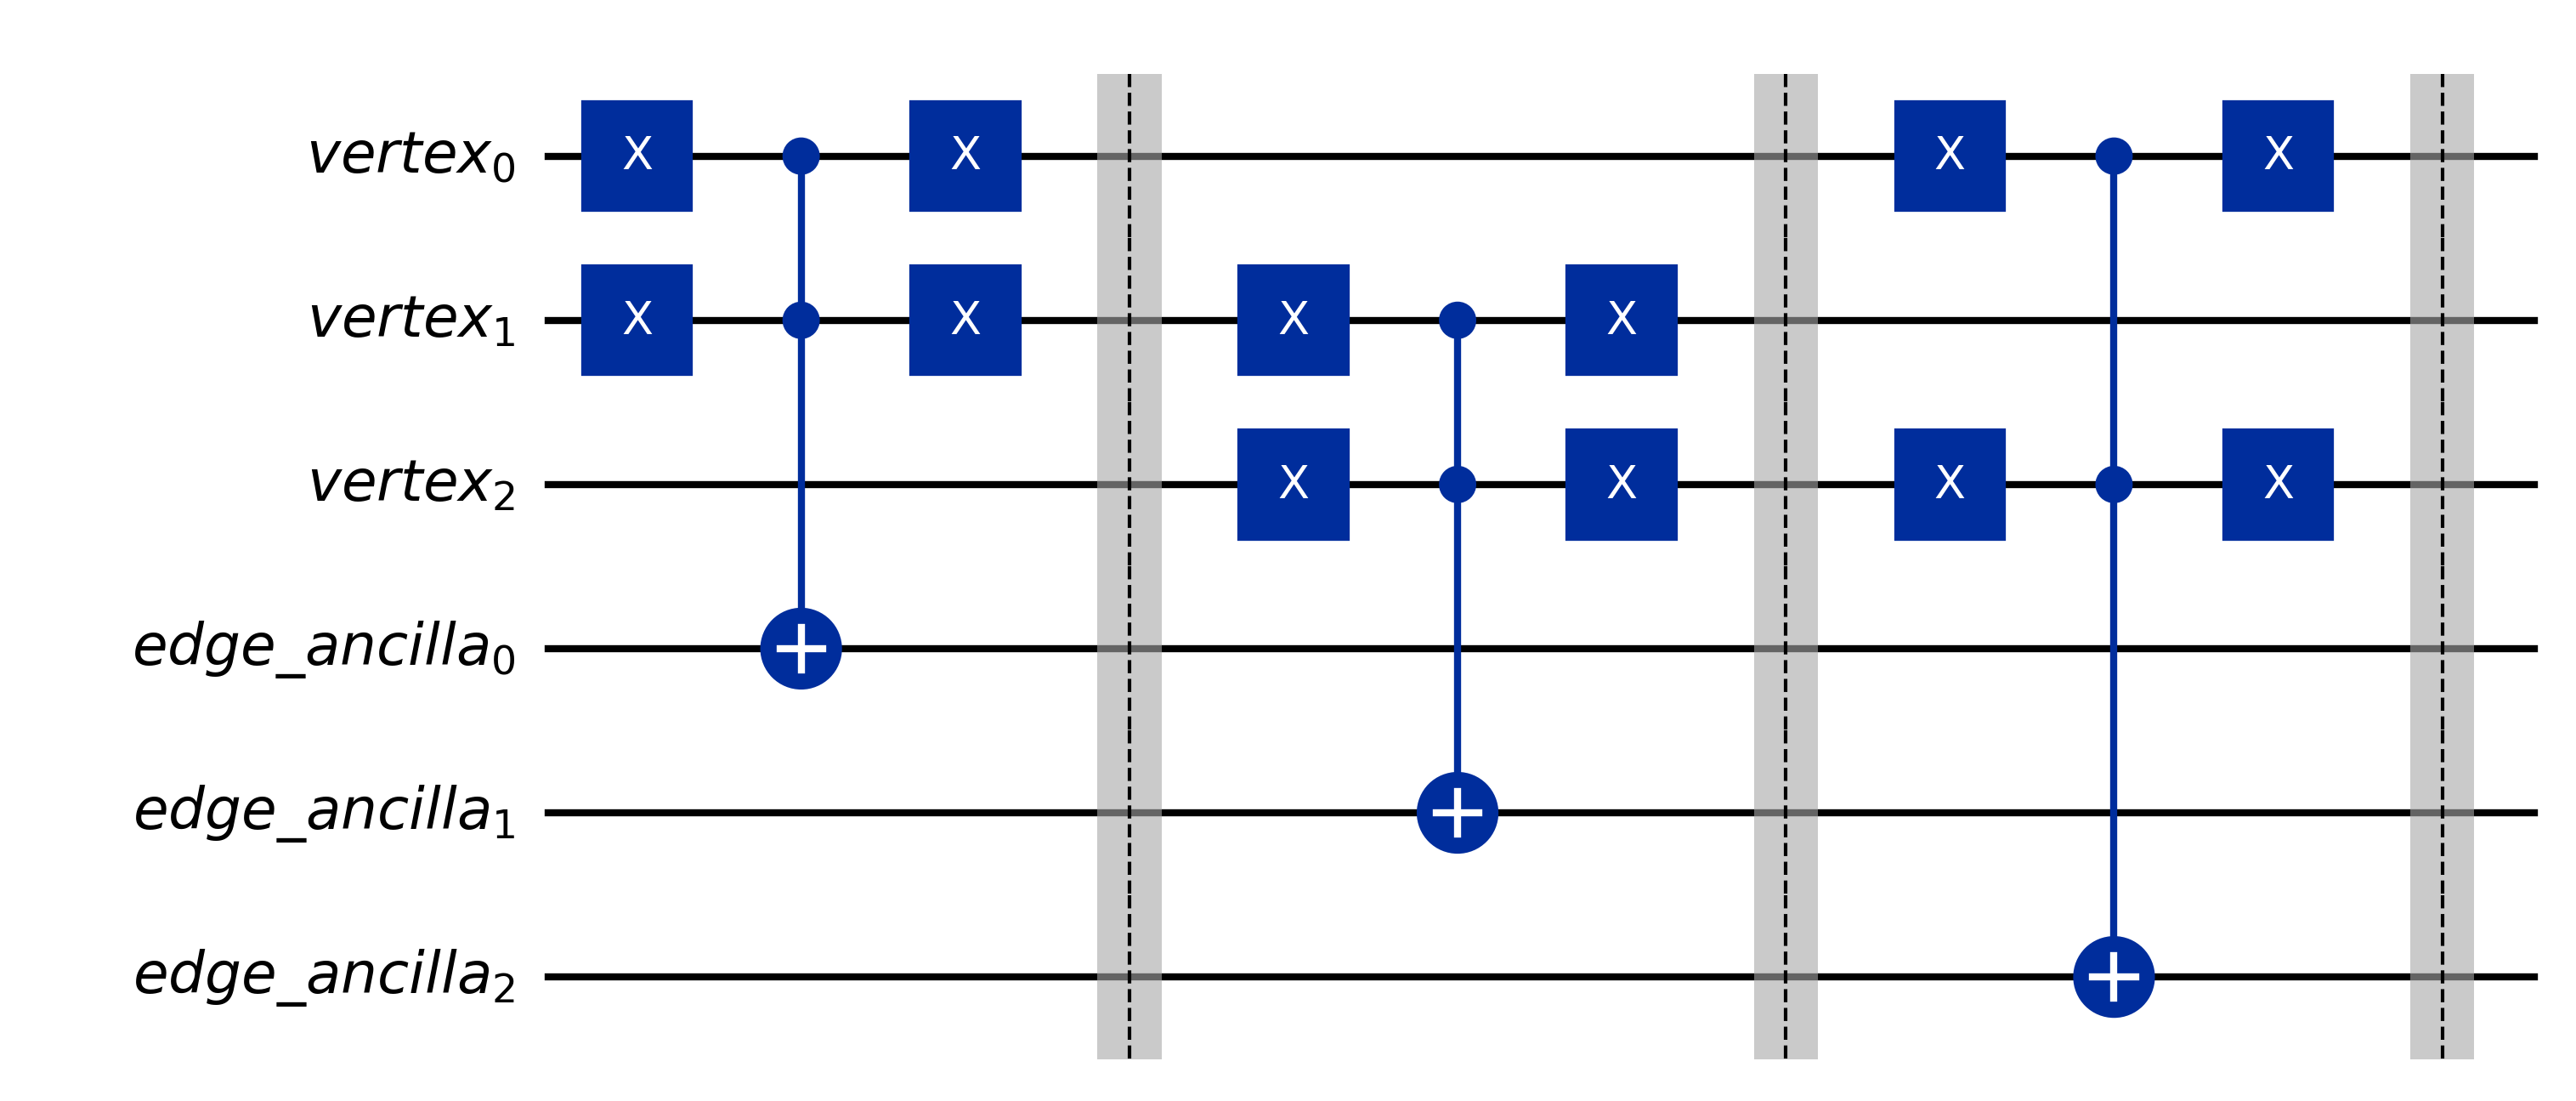
\includegraphics[width=0.5\textwidth]{figures/circuit_edge_check_dicke_01.png}
    \caption{Edge checking circuit for the Dicke-state
    architecture on $K_3$. Each edge ancilla qubit is flipped
    if either incident vertex is selected, followed by a
    multi-controlled-X gate to verify all edges are covered.}
    \label{fig:edge_check_dicke}
\end{figure}

The key insight is that by restricting the search space to
$|D_{\leq k}^n\rangle$, we inherently bias the algorithm
towards smaller vertex covers. If a valid cover of size $k$
exists, the algorithm will find it with higher probability
since the search space has been dramatically reduced.

\paragraph{Diffuser Design}
The diffuser performs reflection around the Dicke state rather
than the uniform superposition. This is implemented as
$U_D = 2|D_{\leq k}^n\rangle\langle D_{\leq k}^n| - I$,
which amplifies the amplitudes of valid vertex covers within
the restricted subspace.

\paragraph{Analysis}
The Dicke-state architecture offers several advantages. First,
it provides geometric filtering of the search space, reducing
the effective problem size from $2^n$ to
$\sum_{i=0}^{k}\binom{n}{i}$. Second, it achieves the fewest
Grover iterations when the optimal cover size $k$ is small
relative to $n$ (i.e., $k \ll n$, which is typical of sparse
graphs where $m \ll n^2$), as the search space reduction
becomes more pronounced. Third, the total qubit requirement
is minimized to $Q_{\mathrm{total}} = n + m + 2$, where the
additional 2 qubits comprise the kickback qubit and the
all-feasible register.

However, this architecture has limitations. The $O(m)$ ancilla
scaling becomes prohibitive for dense graphs. Furthermore, it
cannot natively handle weighted vertex cover since all vertices
are treated equally in the Dicke state preparation. The
Dicke-state architecture achieves optimal efficiency when an
upper bound $k$ on the minimum vertex cover size is known;
without such a bound, the algorithm must start with $k = n$,
reducing the benefit of search space filtering.

% ------ FIX 1: Proposition อยู่นอก proof (consistent กับ weighted) ------
\begin{prop}[Dicke-state Oracle Correctness]
\label{prop:dicke-oracle}
Let $O_{\mathrm{Dicke}}$ be the oracle circuit of the
Dicke-state architecture. For any basis state
$|x\rangle \in \mathrm{supp}(|D^{n}_{\leq k}\rangle)$
with edge ancilla register initialized to
$|0\rangle^{\otimes m}$ and kickback qubit in state
$|-\rangle = \tfrac{1}{\sqrt{2}}(|0\rangle - |1\rangle)$,
the oracle implements:
\begin{equation}
    O_{\mathrm{Dicke}}\,|x\rangle|0\rangle^{\otimes m}|-\rangle
    \;=\;
    (-1)^{\mathrm{valid}(x)}\,
    |x\rangle|0\rangle^{\otimes m}|-\rangle
    \label{eq:dicke-oracle}
\end{equation}
where $\mathrm{valid}(x) = 1$ if and only if $x$ satisfies
the vertex cover constraint
$\forall(u,v) \in E: x_u \vee x_v = 1$, and
$\mathrm{valid}(x) = 0$ otherwise.
\end{prop}

\begin{prf}
We trace the quantum state through four stages of the oracle
circuit.

\medskip
\noindent\textbf{Stage~1 --- Initial state.}
\begin{equation}
    |\psi_0\rangle
    \;=\;
    |x\rangle
    \underbrace{|0\rangle^{\otimes m}}_{\text{edge ancillas}}
    |-\rangle
    \label{eq:dicke-psi0}
\end{equation}

\medskip
\noindent\textbf{Stage~2 --- Edge ancilla flipping.}
For each edge $e_j = (u,v) \in E$, the circuit applies an $X$
gate to ancilla qubit $j$ conditioned on $x_u = 1$
\emph{or} $x_v = 1$, implementing the boolean function
$f_j(x) = x_u \vee x_v$. We verify correctness via the
truth table:

\begin{center}
\begin{tabular}{cc|c|c}
$x_u$ & $x_v$ & $x_u \vee x_v$ & ancilla$_j$ after \\
\hline
0 & 0 & 0 & $|0\rangle$ \\
0 & 1 & 1 & $|1\rangle$ \\
1 & 0 & 1 & $|1\rangle$ \\
1 & 1 & 1 & $|1\rangle$ \\
\end{tabular}
\end{center}

\noindent
The OR function is realized reversibly as:
$\mathrm{CNOT}(u,\,a_j)$,
then $\mathrm{CNOT}(v,\,a_j)$,
then $\mathrm{Toffoli}(u,\,v,\,a_j)$ on $a_j$, which
implements $a_j \leftarrow x_u \vee x_v$ without introducing
garbage qubits. After processing all $m$ edges:
\begin{equation}
    |\psi_1\rangle
    \;=\;
    |x\rangle
    \bigotimes_{j=1}^{m} |f_j(x)\rangle
    \cdot |-\rangle
    \label{eq:dicke-psi1}
\end{equation}

\medskip
\noindent\textbf{Stage~3 --- Phase kickback via
multi-controlled-$X$.}
The multi-controlled-$X$ gate acts on the kickback qubit if
and only if all $m$ edge ancillas are in state $|1\rangle$,
i.e., $\bigwedge_{j=1}^{m} a_j = 1$. By~\eqref{eq:dicke-psi1},
this condition holds if and only if $\mathrm{valid}(x) = 1$.

\smallskip
\noindent\textit{Case~A} --- $x$ is a valid cover
($\mathrm{valid}(x) = 1$): All ancillas are $|1\rangle$,
so the multi-controlled-$X$ flips the kickback qubit:
\begin{equation}
    |-\rangle
    \;=\;
    \tfrac{1}{\sqrt{2}}(|0\rangle - |1\rangle)
    \;\xrightarrow{\;X\;}
    \tfrac{1}{\sqrt{2}}(|1\rangle - |0\rangle)
    \;=\;
    -|-\rangle
    \label{eq:kickback-flip}
\end{equation}
The full system acquires a global phase of $-1$:
\begin{equation}
    |\psi_2\rangle
    = -\,|x\rangle|1\rangle^{\otimes m}|-\rangle
    \label{eq:dicke-psi2-valid}
\end{equation}

\smallskip
\noindent\textit{Case~B} --- $x$ is not a valid cover
($\mathrm{valid}(x) = 0$): At least one ancilla remains
$|0\rangle$; the multi-controlled-$X$ does not fire and no
phase is acquired:
\begin{equation}
    |\psi_2\rangle
    = |x\rangle \bigotimes_{j=1}^{m}|f_j(x)\rangle
    \cdot |-\rangle
    \label{eq:dicke-psi2-invalid}
\end{equation}

\medskip
\noindent\textbf{Stage~4 --- Uncomputation.}
The uncompute step applies the edge-flipping circuit in
reverse order. Since every gate used ($X$, $\mathrm{CNOT}$,
$\mathrm{Toffoli}$) is its own inverse, the uncomputation
exactly reverses Stage~2 and restores every ancilla qubit
to $|0\rangle$:

\smallskip
\noindent\textit{Case~A:}
\begin{equation}
    |\psi_3\rangle
    = -\,|x\rangle|0\rangle^{\otimes m}|-\rangle
    = (-1)^{1}\,|x\rangle|0\rangle^{\otimes m}|-\rangle
    \label{eq:dicke-psi3-valid}
\end{equation}

\noindent\textit{Case~B:}
\begin{equation}
    |\psi_3\rangle
    = |x\rangle|0\rangle^{\otimes m}|-\rangle
    = (-1)^{0}\,|x\rangle|0\rangle^{\otimes m}|-\rangle
    \label{eq:dicke-psi3-invalid}
\end{equation}

\noindent
Combining both cases yields
$O_{\mathrm{Dicke}}\,|x\rangle|0\rangle^{\otimes m}|-\rangle
= (-1)^{\mathrm{valid}(x)}\,
|x\rangle|0\rangle^{\otimes m}|-\rangle$,
as stated in~\eqref{eq:dicke-oracle}. The ancilla register
returns to $|0\rangle^{\otimes m}$ in all cases, confirming
that no residual entanglement is introduced between the
vertex register and the ancilla register after the oracle
call.
\end{prf}

\begin{rem}
\label{rem:or-decomposition}
The OR construction in Stage~2 uses two CNOT gates followed
by a Toffoli gate. If the target hardware requires further
decomposition of the Toffoli gate into two-qubit gates using
intermediate ancillas, those ancillas must also be
uncomputed after each edge. The uncomputation structure
mirrors the forward computation in reverse, which is
standard for reversible circuits and does not affect the
phase kickback result stated above.
\end{rem}

\begin{algorithm}[htbp]
\caption{Dicke-State Architecture}
\label{algo:dicke_state}
\begin{algorithmic}[1]
\STATE \textbf{Registers:} vertex register ($n$) + edge
ancillas ($m$) + kickback (1) + all-feasible (1)
\STATE \textbf{Qubit Requirement:} $Q_{\mathrm{total}} = n + m + 2$
\STATE \textbf{Input:} Graph $G=(V,E)$, pivot threshold $k$,
max iterations $T$
\STATE \textbf{Output:} Minimum vertex cover $V'$
\STATE Prepare registers: vertex ($n$) + edge\_ancillas ($m$)
+ kickback (1) + all-feasible (1)
\STATE Prepare $|D_{\leq k}^n\rangle$ using GDSP~\cite{narisada_concrete_2023}
\FOR{iteration $\gets 1$ \TO $T$}
    \STATE \COMMENT{Oracle: Check if all edges covered}
    \FOR{each edge $e_j = (u,v) \in E$}
        \IF{vertex\_qubit[$u$] = 1 \OR vertex\_qubit[$v$] = 1}
            \STATE Apply X to edge\_ancilla[$j$]
        \ENDIF
    \ENDFOR
    \IF{all edge\_ancillas = 1}
        \STATE Apply CX(all-feasible, kickback) for phase kickback
    \ENDIF
    \STATE \COMMENT{Uncompute oracle}
    \STATE Reverse steps 5--10
    \STATE \COMMENT{Diffuser: Reflect around $|D_{\leq k}^n\rangle$}
    \STATE Apply Dicke-state diffuser
    $U_D = 2|D_{\leq k}^n\rangle\langle D_{\leq k}^n| - I$
\ENDFOR
\STATE \textbf{return} measurement outcome as candidate cover $V'$
\end{algorithmic}
\end{algorithm}

% ------------------------------------------------------------
\subsection{Arithmetic-Based Architecture}

The arithmetic-based solver introduces a fundamentally
different approach by utilizing a computational basis binary
counter to track the number of selected vertices and apply
arithmetic penalties for uncovered edges. This architecture
eliminates the need for per-edge ancilla qubits.

\paragraph{Register Configuration}
The circuit employs the following quantum registers:

\begin{itemize}
    \item \textbf{Vertex Register} ($n$ qubits): Encodes the
    candidate vertex cover, where qubit $|i\rangle = |1\rangle$
    indicates vertex $v_i$ is selected.

    \item \textbf{Counter Register}
    ($\lceil\log_2(n + (n+1)m + 1)\rceil$ qubits): Stores
    the sum of vertex counts plus edge coverage penalties.

    \item \textbf{Pivot Register} (same size as counter):
    Stores the threshold value $k$ against which solutions
    are compared.

    \item \textbf{Kickback Register} (1 qubit): Used for
    phase kickback to mark solutions.

    \item \textbf{Comparator Registers} ($Z$ and $C$, 1 qubit
    each): Working qubits for the Cuccaro comparator.
\end{itemize}

\begin{algorithm}[htbp]
\caption{Arithmetic-Based Architecture}
\label{algo:arithmetic}
\begin{algorithmic}[1]
\STATE \textbf{Registers:} vertex ($n$) + counter + pivot +
kickback (1) + $Z$ (1) + $C$ (1)
\STATE \textbf{Qubit Requirement:}
$Q_{\mathrm{total}} = n + 2\lceil\log_2(n + (n+1)m + 1)\rceil + 3$
\STATE \textbf{Input:} Graph $G=(V,E)$, pivot threshold $k$,
max iterations $T$
\STATE \textbf{Output:} Minimum vertex cover $V'$
\STATE Prepare registers: vertex ($n$) + counter + pivot +
kickback + $Z$ + $C$
\STATE Initialize superposition $|0\rangle^{\otimes n}$
\FOR{iteration $\gets 1$ \TO $T$}
    \STATE \COMMENT{Oracle}
    \STATE Vertex counting: FOR each vertex\_qubit[$i$] = 1:
    \STATE \hspace{1em} Increment counter by 1
    \STATE Apply X to all vertex qubits
    \FOR{each edge $(u,v) \in E$}
        \IF{vertex\_qubit[$u$] = 0 AND vertex\_qubit[$v$] = 0}
            \STATE Add penalty $P = n+1$ to counter
        \ENDIF
    \ENDFOR
    \STATE Apply X to restore vertex qubits
    \STATE Execute Cuccaro comparator: Set $Z = 1$ if
    pivot $>$ counter
    \STATE Apply CX($Z$, kickback) for phase kickback
    \STATE \COMMENT{Uncompute}
    \STATE Reverse steps 5--13
    \STATE \COMMENT{Diffuser: Standard Grover diffuser}
\ENDFOR
\STATE \textbf{return} measurement outcome as candidate
cover $V'$
\end{algorithmic}
\end{algorithm}

\paragraph{Vertex Count Computation}
The number of selected vertices is computed using a
reversible increment circuit controlled by the vertex
register, as shown in Fig.~\ref{fig:popcount_arith}.
For each vertex qubit $i$ in state $|1\rangle$, the counter
register is incremented by 1. This is implemented using a
cascade of controlled-X gates, where each qubit in the
counter is flipped if all lower-order bits and the control
qubit are $|1\rangle$.

\begin{figure}[htbp]
    \centering
    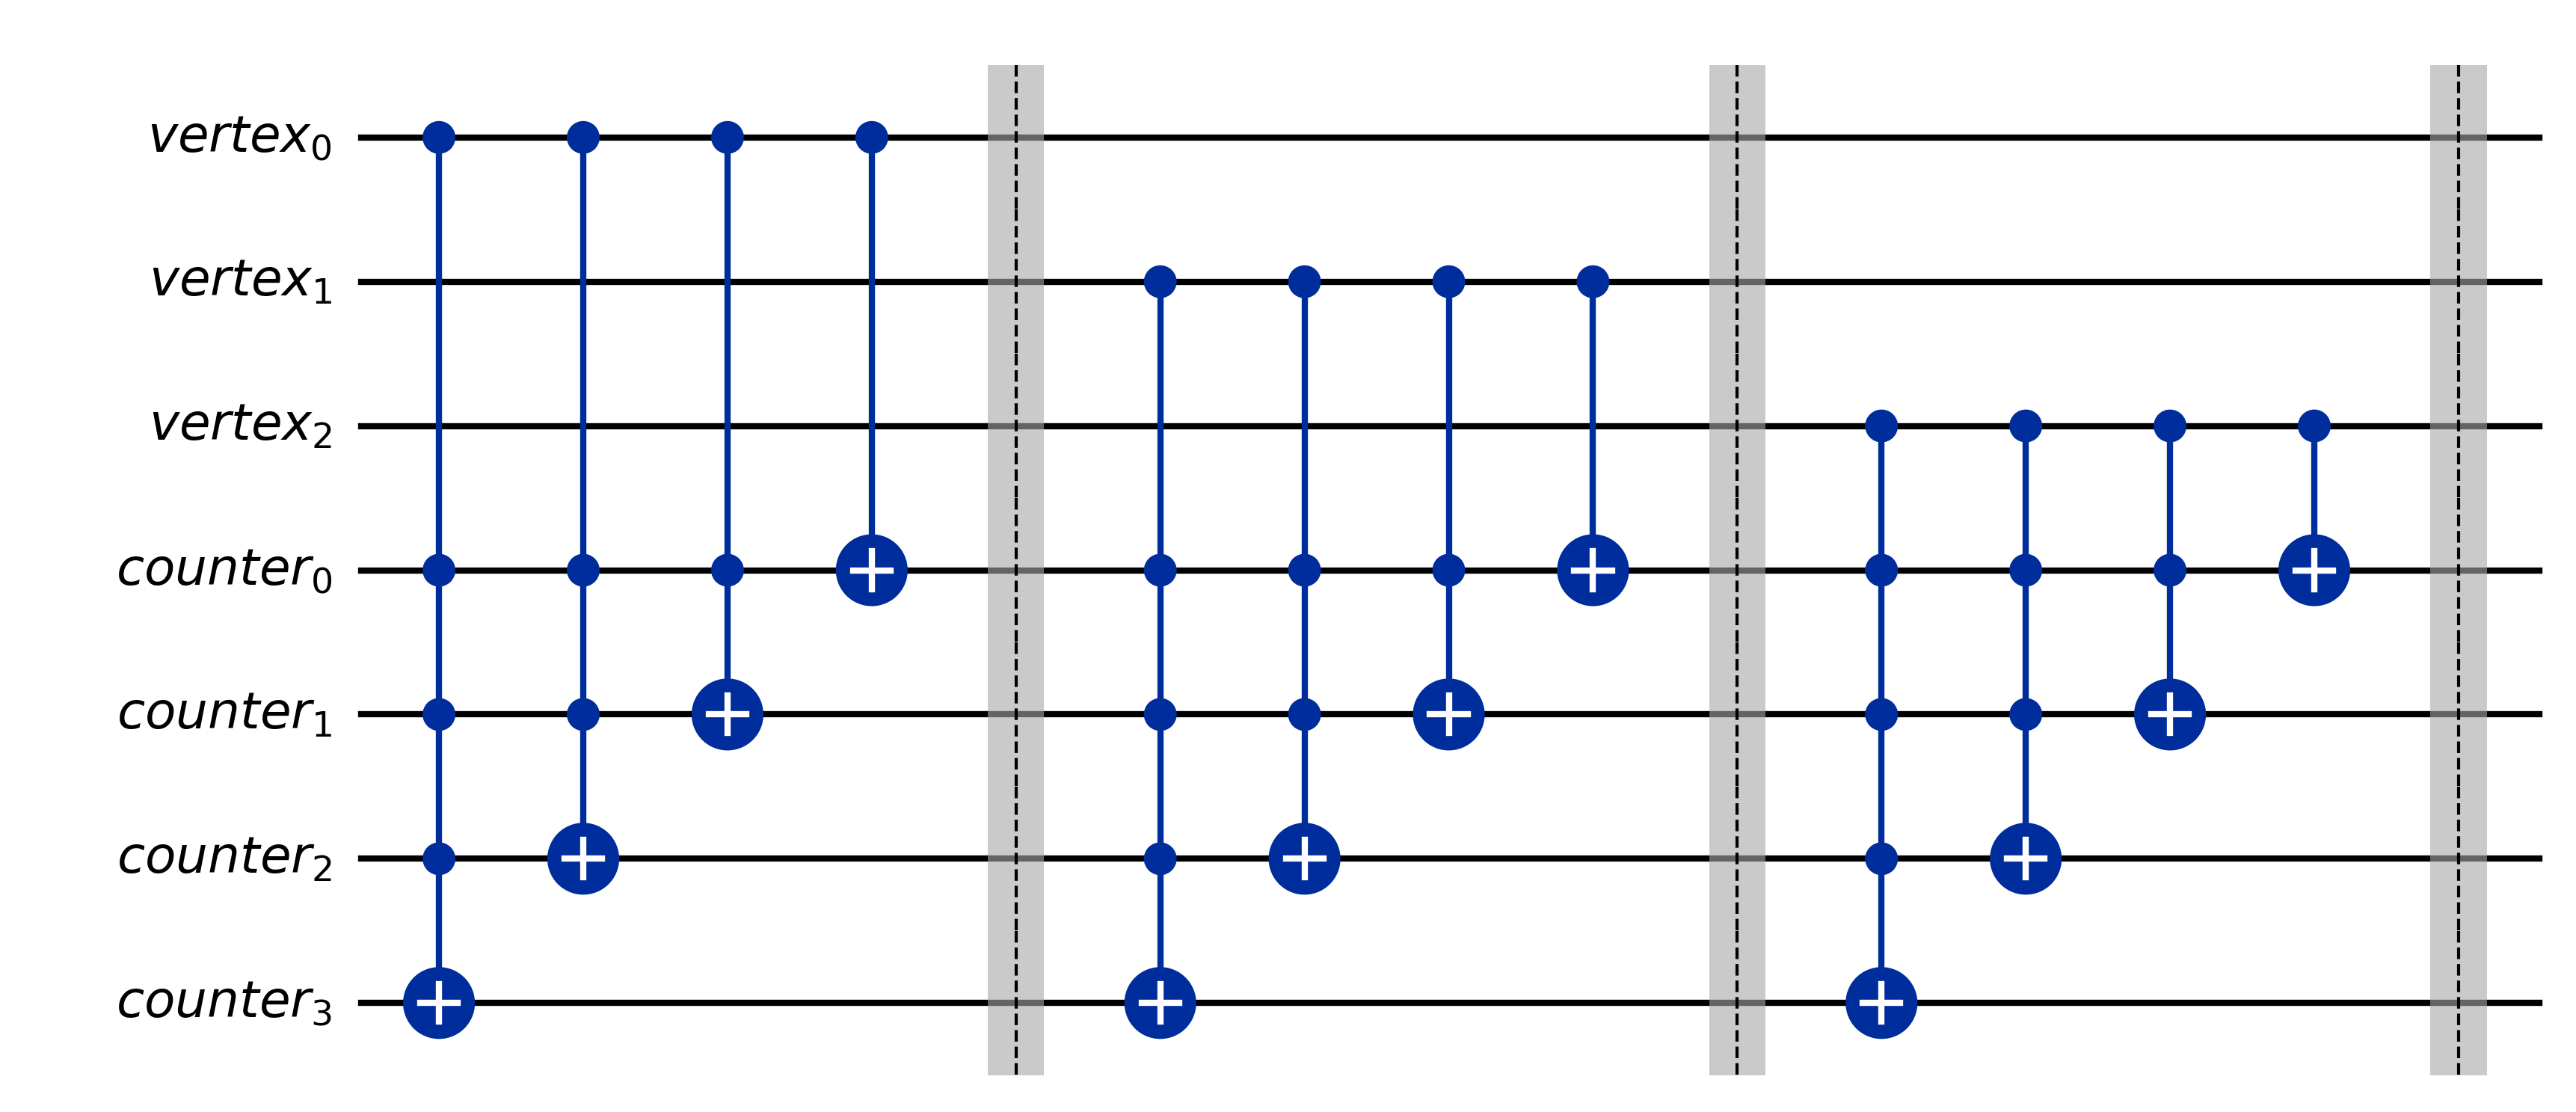
\includegraphics[width=0.5\textwidth]{figures/circuit_popcount_arith_01.png}
    \caption{Popcount (vertex counting) circuit for the
    arithmetic architecture on $K_3$. The ripple-carry
    incrementer uses multi-controlled-X gates to increment
    the counter for each selected vertex.}
    \label{fig:popcount_arith}
\end{figure}

\paragraph{Edge Coverage Penalty Adder}
For each edge $(u,v) \in E$, if both vertices are unselected
(qubits $u$ and $v$ are $|0\rangle$), a penalty $P = n+1$
is added to the counter register (as shown in
Fig.~\ref{fig:penalty_arith}). Since the maximum pivot value
is $n+1$, this ensures that any uncovered edge causes the
counter to exceed any valid pivot value, effectively
invalidating the solution.

The penalty addition is performed by decomposing $P$ into
binary representation and applying controlled increments to
the counter. Since $P = n+1$ requires at most
$\lfloor\log_2(n+1)\rfloor + 1 = O(\log n)$ bits, the
penalty addition requires $O(m \cdot \log n)$ operations.

\begin{figure}[htbp]
    \centering
    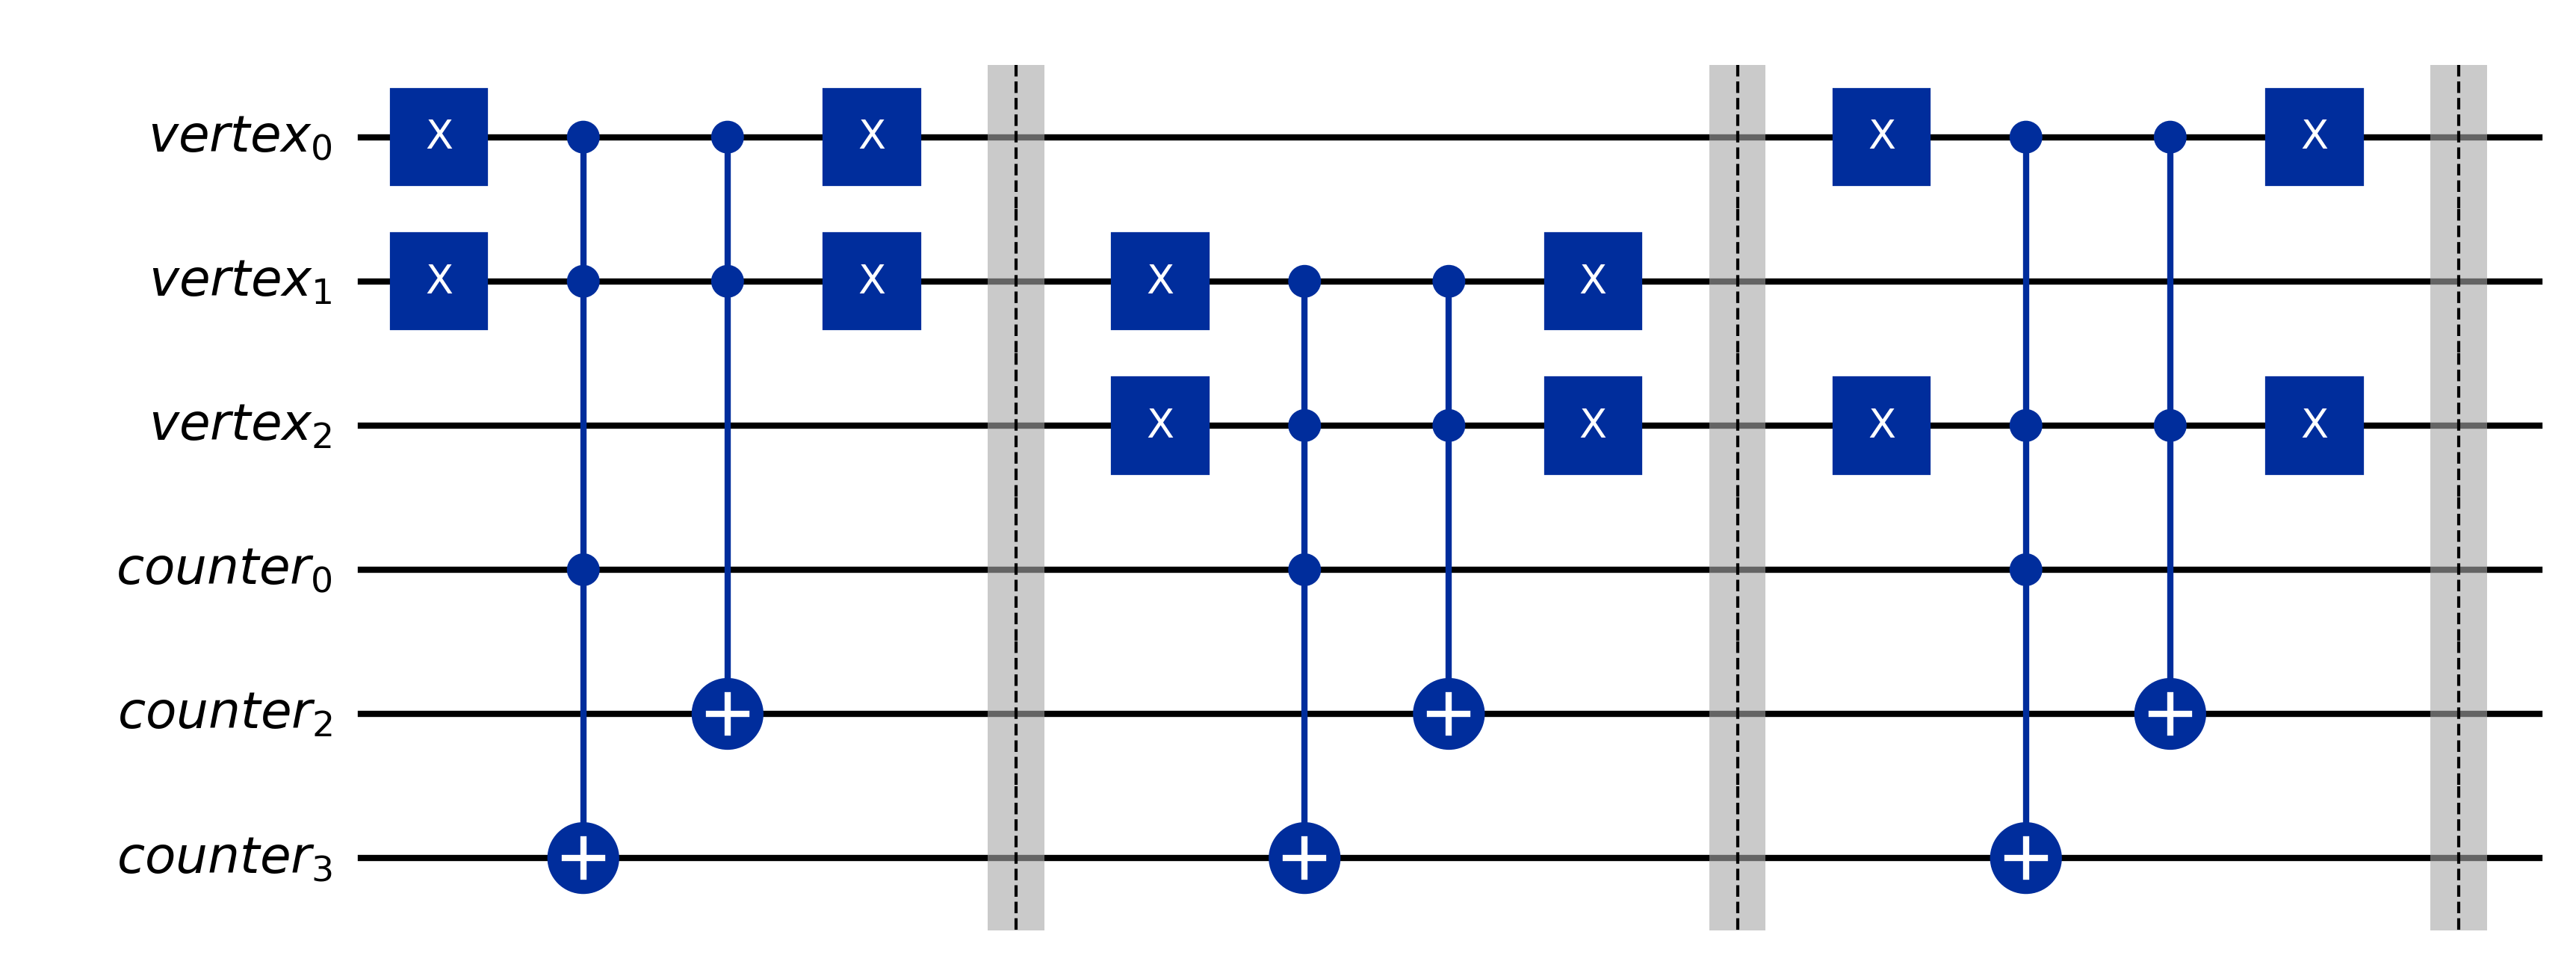
\includegraphics[width=0.5\textwidth]{figures/circuit_penalty_arith_01.png}
    \caption{Penalty adder circuit for the arithmetic
    architecture on $K_3$. When both vertices of an edge are
    unselected (state $|0\rangle$), a penalty value of $n+1$
    is added to the counter using binary-decomposed controlled
    increments.}
    \label{fig:penalty_arith}
\end{figure}

\paragraph{Cuccaro Comparator}
We employ the Cuccaro comparator~\cite{benchasattabuse_quantum_2019}
to determine whether the counter value exceeds the pivot.
The comparator takes two $t$-bit numbers $A$ (pivot) and
$B$ (counter) and sets the $Z$ qubit to 1 if $A > B$.
The circuit uses the MAJ (majority) and IMAJ (inverse
majority) gate sequences:
\begin{enumerate}
    \item Initialize: Apply $X$ to all $B$ qubits.
    \item Forward MAJ: Cascade $\mathrm{MAJ}(A_i, B_i, C_i)$
    for $i = 0$ to $t-1$.
    \item Comparison: $\mathrm{CX}(A_{t-1}, Z)$ stores the
    result.
    \item Backward IMAJ: Cascade $\mathrm{IMAJ}(A_i, B_i,
    C_i)$ for $i = t-1$ down to 0.
    \item Uncompute: Apply $X$ to all $B$ qubits.
\end{enumerate}

\paragraph{Oracle Operation}
The complete oracle operation proceeds as follows:
\begin{enumerate}
    \item Compute vertex count into counter register.
    \item Apply $X$ to all vertex qubits
    (flipping $|0\rangle \to |1\rangle$ and vice versa).
    \item For each uncovered edge, add penalty $P = n+1$ to
    counter.
    \item Apply $X$ again to restore original vertex states.
    \item Execute Cuccaro comparator to check if counter
    $<$ pivot.
    \item Apply phase kickback: $\mathrm{CX}(Z,
    \mathrm{kickback})$.
    \item Uncompute the comparator, penalty adder, and vertex
    counter in reverse order.
\end{enumerate}

\paragraph{Analysis}
The arithmetic architecture offers significant advantages for
dense graphs. The edge validation overhead scales as
$O(\log m)$ instead of $O(m)$, making it more scalable for
graphs with many edges. The total qubit requirement is:
\begin{equation}
    Q_{\mathrm{total}}
    = n + 2\,\lceil\log_2(n + (n+1)m + 1)\rceil + 3
    \label{eq:arith-qubits}
\end{equation}

The trade-off is increased circuit depth due to the
sequential nature of the penalty addition and the carry
propagation in the comparator. Each Grover iteration
requires multiple passes through the counter circuit,
penalty adder, and comparator, resulting in deeper circuits
compared to the Dicke-state approach.

This architecture assumes uniform vertex weights (each
vertex contributes 1 to the count) and finds minimum
cardinality vertex covers through iterative pivot testing.
This iterative approach can be accelerated using Skip-K
optimization to skip redundant pivot values.

% ------ FIX 2: proof อยู่นอก proposition (consistent กับ dicke + weighted) ------
\begin{prop}[Arithmetic Oracle Correctness]
\label{theo:arithmetic_correctness}
For any candidate vertex subset $x \in \{0,1\}^n$ and pivot
value $p \in [1, n+1]$, the arithmetic oracle marks $x$ as a
valid solution \textbf{iff}:
\begin{enumerate}
    \item $x$ is a valid vertex cover (every edge $(u,v) \in E$
    has at least one endpoint selected), and
    \item the number of selected vertices $|x| \leq p-1$.
\end{enumerate}
\end{prop}

\begin{prf}
The oracle computes:
\begin{equation}
    \mathrm{counter}(x)
    = \sum_{i=1}^n x_i
    + \sum_{(u,v) \in E} P \cdot (1-x_u)(1-x_v)
    \label{eq:arith-counter}
\end{equation}
where $P = n+1$ is the penalty for uncovered edges.

\noindent(\textit{Forward:}) If $x$ is valid with
$|x| \leq p-1$, then every edge is covered so
$(1-x_u)(1-x_v) = 0$ for all edges. Thus
$\mathrm{counter}(x) = |x| \leq p-1 < p$. Since counter
$< p$, the Cuccaro comparator sets $Z = 1$, triggering phase
kickback to mark this as a valid solution.

\noindent(\textit{Reverse:}) If the oracle marks $x$ as
valid, then counter $< p$. Since $p \leq n+1$ and each
uncovered edge adds penalty $P = n+1 \geq p$, at least one
uncovered edge would make counter $\geq n+1 \geq p$.
Therefore, all edges must be covered. With no penalties,
counter $= |x| < p$ implies $|x| \leq p-1$.
\end{prf}

% ------------------------------------------------------------
\subsection{Weighted Arithmetic Architecture}

The weighted arithmetic architecture generalizes the
arithmetic approach to support heterogeneous vertex weights,
making it suitable for the Weighted Minimum Vertex Cover
(WMVC) problem. Like the unweighted version, it can leverage
Skip-K optimization to skip redundant pivot values during
the iterative search.

\paragraph{Weighted Sum Computation}
Unlike the unweighted vertex count that adds 1 for each
selected vertex, the weighted version adds $w_i$ (the weight
of vertex $v_i$) to the counter when qubit $i$ is in state
$|1\rangle$. This is implemented by decomposing each weight
$w_i$ into its binary representation and applying controlled
increments accordingly.

For example, if vertex $v_2$ has weight $w_2 = 5$
(binary 101), we add 1 to counter bits 0 and 2 when qubit 2
is $|1\rangle$. This allows arbitrary integer weights to be
represented.

\paragraph{Penalty Calculation}
The penalty for uncovered edges becomes
$P = \sum_{i=1}^{n} w_i + 1$. Since the maximum possible
vertex weight sum is $\sum_{i=1}^{n} w_i$, we have
$P = \sum w_i + 1 > \sum w_i$, ensuring that any uncovered
edge causes the total to exceed any valid cover weight.

The counter size is determined by:
\begin{equation}
    \mathrm{counter\_size}
    = \left\lceil\log_2\!\left(
        \textstyle\sum w_i
        + \bigl(\textstyle\sum w_i + 1\bigr)m + 1
      \right)\right\rceil
    \label{eq:weighted-counter-size}
\end{equation}

\paragraph{Iterative Search with Pivot Testing}
The weighted solver uses an iterative approach similar to the
unweighted version. Starting from a pivot value of
$\sum w_i + 1$ (greater than any possible cover), it tests
progressively smaller pivots. At each pivot value $k$, the
Grover algorithm amplifies states representing vertex covers
with total weight $\leq k$.

The algorithm terminates when no solution is found at a
given pivot, indicating that the minimum cover has weight
$\mathrm{pivot} - 1$.

See Algorithm~\ref{algo:skip_k} for the unified Skip-K
optimization that applies to all three architectures.

\paragraph{Skip-K Optimization}
\label{para:skip-k}
A major challenge in finding the absolute minimum cover size
is the lack of a priori knowledge regarding the exact optimal
value. We introduce a classical optimization that leverages
measurement results to skip redundant pivot values. The
Skip-K optimization applies to all three architectures and
works as follows:

\begin{enumerate}
    \item After running Grover's algorithm at pivot $k$,
    measure the quantum state.
    \item If a valid vertex cover of weight $w$ is found
    (where $w < k$), we know the minimum cover has weight
    $\leq w$.
    \item Instead of testing all intermediate pivot values,
    skip directly to $w$, using $w$ as the new upper bound
    on the minimum cover weight.
    \item This can reduce the number of Grover executions
    from $O(\sum w_i)$ to $O(w_{\min})$ in the best case.
\end{enumerate}

The Skip-K optimization is particularly effective when:
\begin{itemize}
    \item Good solutions are found early in the search
    process.
    \item The distribution of vertex weights allows for large
    skip intervals.
\end{itemize}

\paragraph{Analysis}
The weighted arithmetic architecture is the most
general-purpose solution among our three approaches. It
successfully handles arbitrary vertex weights and provides a
clear path to the minimum weight cover through deterministic
pivot testing.

The qubit requirement becomes:
\begin{equation}
    Q_{\mathrm{total}}
    = n + 2\,\left\lceil\log_2\!\left(
        \textstyle\sum w_i
        + \bigl(\textstyle\sum w_i + 1\bigr)m + 1
      \right)\right\rceil + 3
    \label{eq:weighted-qubits}
\end{equation}

While the circuit depth increases slightly compared to the
unweighted version due to the more complex weighted sum
computation, the asymptotic scaling remains efficient.
However, a naive iterative search for the optimal solution
would require testing up to $\sum w_i$ pivot values, which
is computationally expensive. To compensate for this
increased search space, the \textbf{Skip-K optimization}
(detailed in Section~\nameref{para:skip-k}) becomes highly
critical for this architecture. By leveraging classical
measurement feedback to skip redundant pivot values, this
approach reduces the number of Grover executions from
$O(\sum w_i)$ down to $O(w_{\min})$ in the best case.
Furthermore, this mechanism is particularly advantageous in
practical implementations, as inherent noise in NISQ devices
occasionally produces valid, lower-weight solutions even when
testing at high pivot values, thereby triggering larger
optimization skips.

Ultimately, this architecture is the only one capable of
correctly identifying minimum covers in weighted instances,
making it essential for real-world applications where
vertices have heterogeneous costs (e.g., resource
allocation, network design).

\begin{prop}[Weighted Arithmetic Oracle Correctness]
\label{prop:weighted-oracle}
For any candidate vertex subset $x \in \{0,1\}^n$ and pivot
value $p \in \bigl[1,\,\sum_{i=1}^{n} w_i + 1\bigr]$, the
weighted arithmetic oracle marks $x$ as a valid solution if
and only if:
\begin{enumerate}
    \item $x$ is a valid vertex cover, i.e., every edge
    $(u,v) \in E$ has at least one endpoint selected
    ($x_u \vee x_v = 1$), and
    \item the total weight of selected vertices satisfies
    $W(x) = \sum_{i=1}^{n} w_i x_i \leq p - 1$.
\end{enumerate}
\end{prop}

\begin{lemma}[Weighted Penalty Sufficiency]
\label{lem:weighted-penalty}
Let $P_w = \sum_{i=1}^{n} w_i + 1$. For any
$x \in \{0,1\}^n$ with at least one uncovered edge,
\begin{equation}
    \mathrm{counter}(x)
    \;\geq\;
    P_w
    \;=\;
    \sum_{i=1}^{n} w_i + 1
    \;>\;
    \sum_{i=1}^{n} w_i
    \;\geq\;
    p - 1
    \label{eq:penalty-sufficiency}
\end{equation}
so the Cuccaro comparator does not mark $x$ as a valid
solution.
\end{lemma}

\begin{prf}[Proof of Lemma~\ref{lem:weighted-penalty}]
The weighted oracle computes:
\begin{equation}
    \mathrm{counter}(x)
    \;=\;
    \underbrace{\sum_{i=1}^{n} w_i x_i}_{W(x)\,\geq\,0}
    \;+\;
    \underbrace{
        \sum_{(u,v)\in E}
        P_w \cdot (1-x_u)(1-x_v)
    }_{\text{penalty for uncovered edges}}
    \label{eq:weighted-counter}
\end{equation}
If at least one edge $(u,v)$ is uncovered, then
$(1-x_u)(1-x_v) = 1$ for that edge, contributing
$P_w = \sum_{i=1}^{n} w_i + 1$ to the counter. Since
$W(x) \geq 0$, we have $\mathrm{counter}(x) \geq P_w$.

The maximum valid cover weight corresponds to selecting all
vertices, giving $\sum_{i=1}^{n} w_i$. Therefore any
meaningful pivot satisfies $p \leq \sum_{i=1}^{n} w_i + 1$,
which means $p - 1 \leq \sum_{i=1}^n w_i < P_w \leq
\mathrm{counter}(x)$. Hence counter$(x) \geq p$, and the
Cuccaro comparator sets $Z = 0$, so no phase kickback occurs.
\end{prf}

\begin{prf}[Proof of Proposition~\ref{prop:weighted-oracle}]
We trace the oracle computation using the counter expression
in~\eqref{eq:weighted-counter}.

\medskip
\noindent\textbf{Initial state.}
\begin{equation}
    |\psi_0\rangle
    \;=\;
    |x\rangle\,|0\rangle_{\mathrm{counter}}\,
    |p\rangle_{\mathrm{pivot}}\,
    |0\rangle_{Z}\,|-\rangle_{\mathrm{kick}}
    \label{eq:w-psi0}
\end{equation}

\medskip
\noindent\textbf{Forward direction ($\Rightarrow$).}
Suppose $x$ is a valid vertex cover with $W(x) \leq p-1$.
Then every edge is covered, so $(1-x_u)(1-x_v) = 0$ for all
$(u,v) \in E$. From~\eqref{eq:weighted-counter}:
\begin{equation}
    \mathrm{counter}(x)
    = W(x) + 0
    = W(x)
    \leq p - 1
    < p
    \label{eq:w-forward}
\end{equation}
Since counter$(x) < p$, the Cuccaro comparator sets $Z = 1$,
and the subsequent $\mathrm{CX}(Z,\mathrm{kick})$ gate
flips the kickback qubit $|-\rangle \to -|-\rangle$,
acquiring a phase of $-1$. After uncomputation of the
comparator, penalty adder, and weighted sum circuit (in
reverse order), all ancilla registers return to their
initial states. The net effect on the vertex register is:
\begin{equation}
    |x\rangle \;\longmapsto\; -\,|x\rangle
    = (-1)^{1}\,|x\rangle
    \label{eq:w-phase-valid}
\end{equation}

\medskip
\noindent\textbf{Reverse direction ($\Leftarrow$).}
Suppose the oracle marks $x$ as valid, i.e.,
counter$(x) < p$. By Lemma~\ref{lem:weighted-penalty}, if
any edge were uncovered, counter$(x) \geq P_w \geq p$,
contradicting counter$(x) < p$. Therefore all edges must be
covered and $x$ is a valid vertex cover. With no uncovered
edges, the penalty terms vanish and counter$(x) = W(x)$.
Since counter$(x) < p$, we obtain $W(x) \leq p - 1$.

\medskip
\noindent\textbf{Uncomputation completeness.}
Each subroutine weighted sum computation, penalty adder,
and Cuccaro comparator is implemented as a reversible
circuit. Their uncomputation steps apply each gate in
reverse order and restore all registers exactly to
$|0\rangle$. Consequently, after the oracle call, no
register outside the vertex register retains any information
about $x$, and the phase in~\eqref{eq:w-phase-valid} is the
sole effect on the system state.
\end{prf}


\begin{rem}
\label{rem:weighted-special-case}
Proposition~\ref{prop:weighted-oracle} strictly generalizes
Proposition~\ref{theo:arithmetic_correctness} (unweighted
arithmetic oracle). Setting $w_i = 1$ for all $i$ recovers
$W(x) = |x|$ (Hamming weight) and $P_w = n + 1 = P$, which
are exactly the quantities used in the unweighted oracle.
\end{rem}

\begin{rem}
\label{rem:superposition}
Propositions~\ref{prop:dicke-oracle}
and~\ref{prop:weighted-oracle} are stated for computational
basis states $|x\rangle$. By linearity of quantum mechanics,
both oracles act correctly on arbitrary superpositions: for
$|\psi\rangle = \sum_{x} \alpha_x |x\rangle$,
\begin{equation}
    O \!\left(\sum_{x} \alpha_x |x\rangle\right)
    |0\rangle^{\otimes \mathrm{anc}}\,|-\rangle
    \;=\;
    \sum_{x} \alpha_x\,(-1)^{\mathrm{valid}(x)}
    |x\rangle\,|0\rangle^{\otimes \mathrm{anc}}\,|-\rangle
    \label{eq:superposition-correctness}
\end{equation}
since all ancilla and kickback registers return to their
initial states for every basis state $|x\rangle$
independently. This confirms that the amplitude
amplification mechanism of Grover's algorithm operates as
intended across the entire superposition.
\end{rem}


\begin{algorithm}[htbp]
\caption{Skip-K Optimization (Unified)}
\label{algo:skip_k}
\begin{algorithmic}[1]
\STATE \textbf{Input:} Graph $G=(V,E)$,
architecture $\in \{$\textit{Dicke-State},
\textit{Arithmetic}, \textit{Weighted}$\}$,
vertex weights $w_i$, initial pivot $k_{\max}$
\STATE \textbf{Output:} Minimum vertex cover weight $w_{\min}$
\STATE $k \gets k_{\max}$
\WHILE{$k > 0$}
    \STATE Run Grover's algorithm with selected architecture
    and pivot $k$
    \STATE Measure quantum state, obtaining candidate cover
    weight $w$
    \IF{$w < k$ \AND $w$ is valid cover}
        \STATE $k \gets w$
        \COMMENT{$w$ is new upper bound on $w_{\min}$;
        skip testing pivots $k-1, \ldots, w+1$}
    \ELSE
        \STATE $k \gets k - 1$
    \ENDIF
\ENDWHILE
\STATE \textbf{return} $w_{\min} = k$
\end{algorithmic}
\end{algorithm}

% ============================================================
\section{Formal Analysis}
\label{sec:formal_analysis}

We now provide formal analysis for key properties of our
architectures, including the correctness of the arithmetic
oracle and the Skip-K optimization.

% ------------------------------------------------------------
\subsection{Sparse Graph Definition}

Before analyzing Skip-K, we first formalize the notion of
sparse graphs used throughout this paper:

\begin{dfin}
\label{def:sparse}
A graph $G = (V,E)$ with $n = |V|$ vertices and $m = |E|$
edges is considered \textbf{sparse} if $m = o(n^2)$,
equivalently $m \ll n^2$. In practice, this includes graphs
where $m = O(n)$ or $m = O(n \log n)$.
\end{dfin}

This definition justifies our claims about Dicke-state
efficiency in Section~\ref{sec:dicke_state}, where the
condition $k \ll n$ typically coincides with sparse graphs
($m \ll n^2$).

\subsection{Skip-K Optimization Analysis}
\label{sec:skipk_analysis}

We analyze the Skip-K optimization formally, establishing
termination, best-case and worst-case complexity, and
correctness guarantees under both ideal and noisy conditions.

% ------ Proposition: best-case ------
\begin{prop}[Skip-K Best-Case Complexity]
\label{theo:skipk}
Let $w_{\min}$ be the minimum vertex cover weight. Given an
initial pivot $k_{\max} \geq \sum_i w_i$, the Skip-K
optimization reduces the number of Grover executions from
$O(\sum_i w_i)$ to $O(w_{\min})$ in the best case.
\end{prop}

\begin{prf}
The naive iterative approach tests all pivot values from
$k_{\max}$ down to 1, requiring up to
$k_{\max} = O(\sum_i w_i)$ executions. With Skip-K, which
extends the classical feedback technique of D\"{u}rr and
Hoyer~\cite{durr_quantum_1999} to pivot selection, at each
iteration:
\begin{enumerate}
    \item We run Grover's algorithm at pivot $k$.
    \item If we obtain a valid cover of weight $w < k$,
          we know $w_{\min} \leq w$.
    \item We skip directly to $k = w$, skipping all
          intermediate values.
\end{enumerate}
In the best case, we find a solution with weight $w_{\min}$
on the first successful iteration, requiring only
$O(w_{\min})$ executions (the remaining gap from $k_{\max}$
to $w_{\min}$ is skipped in one step).
\end{prf}

% ------ Corollary: worst-case (เดิมมีอยู่แล้ว) ------
\begin{cor}
\label{cor:skipk-worst}
The worst-case complexity of Skip-K remains
$O(\sum_i w_i)$, occurring when valid covers are discovered
only at the final iteration (i.e., no solution is found
until $k = w_{\min}$).
\end{cor}

\begin{prf}
In the worst case, valid covers are discovered only when
$k = w_{\min}$, so no skipping occurs. The algorithm must
test each intermediate value from $k_{\max}$ down to
$w_{\min}$, requiring $O(k_{\max} - w_{\min}) =
O(\sum_i w_i)$ executions.
\end{prf}

% ------ Termination Proof ------
\begin{prop}[Skip-K Termination]
\label{prop:skipk-termination}
Algorithm~\ref{algo:skip_k} terminates within at most
$k_{\max}$ iterations for any input graph $G$ and any
sequence of measurement outcomes.
\end{prop}

\begin{prf}
We show that the pivot variable $k$ strictly decreases by
at least 1 at every iteration of the \textbf{while} loop,
and that $k$ is lower-bounded by 0.

At each iteration, exactly one of two cases applies:
\begin{itemize}
    \item \textit{Skip branch} (line 8 of
    Algorithm~\ref{algo:skip_k}): a valid cover of weight
    $w < k$ is found, so $k \leftarrow w \leq k - 1$.
    Thus $k$ decreases by at least 1.

    \item \textit{Decrement branch} (line 10):
    no valid cover with weight $< k$ is found, so
    $k \leftarrow k - 1$. Thus $k$ decreases by exactly 1.
\end{itemize}
In both cases $k$ decreases by at least 1 per iteration.
Since $k$ is initialized to $k_{\max}$ and is a
non-negative integer, the loop executes at most $k_{\max}$
iterations before $k = 0$ and the loop condition $k > 0$
becomes false. Therefore Algorithm~\ref{algo:skip_k}
terminates within at most $k_{\max}$ iterations.
\end{prf}

% ------ Remark — noise / correctness under NISQ ------
\begin{rem}[Correctness Under Noise]
\label{rem:skipk-noise}
The correctness guarantee of
Proposition~\ref{theo:skipk} assumes that every measurement
outcome faithfully reflects the quantum state, i.e.,
measurements are error-free. Under realistic NISQ conditions,
two failure modes may arise:

\begin{enumerate}
    \item \textit{False-positive skip}: noise causes the
    circuit to collapse to a low-weight state $w$ that is
    \emph{not} a valid vertex cover, yet passes the validity
    check. Skip-K then sets $k \leftarrow w$, potentially
    skipping the true minimum $w_{\min}$ if
    $w < w_{\min}$.

    \item \textit{False-negative}: noise destroys the
    amplitude amplification effect, causing no valid cover
    to be observed at a pivot where one exists. This forces
    the decrement branch and increases the total number of
    executions.
\end{enumerate}

To mitigate false-positive skips, we recommend running
Grover's algorithm $r \geq 3$ times at each pivot value and
adopting the measurement outcome only if a majority
($\lceil r/2 \rceil$) of runs return the same valid cover
weight. This majority-vote strategy reduces the
false-positive probability from $\epsilon$ per run to
$O(\epsilon^{\lceil r/2 \rceil})$ at the cost of
multiplying the total number of Grover circuit executions
by $r$.

We note that Section~\ref{sec:discussion} observes
noise-induced collapses to low-weight covers as a
\emph{heuristic} advantage. This observation is
complementary, not contradictory: occasional lucky collapses
can trigger large beneficial skips, but relying on them
without majority voting risks skipping past the true
optimum. In practice, the majority-vote threshold $r$
should be chosen based on the estimated gate fidelity of
the target device.
\end{rem}

% ------ Quantitative Example ------
\begin{rem}[Quantitative Comparison: Skip-K vs.\ Naive Search]
\label{rem:skipk-example}
To illustrate the practical advantage of Skip-K, consider
three representative scenarios. In each case, the naive
iterative search tests every pivot from $k_{\max}$ down to
$w_{\min}$, requiring exactly $k_{\max} - w_{\min} + 1$
Grover executions. Skip-K reduces this in the best case to
$O(w_{\min})$ executions as established in
Proposition~\ref{theo:skipk}.

Table~\ref{tab:skipk-comparison} summarizes the comparison.
The speedup ratio is defined as:
\begin{equation}
    \mathrm{Speedup}
    \;=\;
    \frac{k_{\max} - w_{\min} + 1}{\text{Skip-K executions
    (best case)}}
    \;=\;
    \frac{k_{\max} - w_{\min} + 1}{w_{\min} + 1}
    \label{eq:skipk-speedup}
\end{equation}

\begin{table}[htbp]
\centering
\caption{Quantitative comparison of Skip-K versus naive
iterative search across three representative scenarios.
Best-case Skip-K executions $= w_{\min} + 1$ (one
execution to discover $w_{\min}$, then $w_{\min}$
decrements to confirm no lighter cover exists).}
\label{tab:skipk-comparison}
\begin{tabular}{lcccccc}
\hline
\textbf{Scenario} &
$n$ & $\sum w_i$ & $w_{\min}$ & $k_{\max}$ &
\textbf{Naive} & \textbf{Skip-K (best)} \\
\hline
Unweighted sparse
  & 20 & 20  & 4  & 21  & 18  & 5   \\
Weighted moderate
  & 10 & 100 & 15 & 101 & 87  & 16  \\
Weighted high-spread
  & 10 & 1000 & 10 & 1001 & 992 & 11 \\
\hline
\end{tabular}
\end{table}

The speedup is most pronounced in the high-spread scenario,
where $k_{\max}/w_{\min} = 100$ and Skip-K requires only
11 executions compared to 992 for naive search---a
$90\times$ reduction. This highlights that Skip-K is
especially valuable for weighted instances where the sum
of vertex weights is large but the optimal cover uses only
a few low-weight vertices.

Conversely, in the unweighted sparse scenario the speedup
is more modest ($3.6\times$) because $k_{\max} = n$ and
$w_{\min}$ is already a substantial fraction of $n$. In the
worst case (Corollary~\ref{cor:skipk-worst}), all three
scenarios revert to the naive count.
\end{rem}

\begin{rem}
\label{rem:skipk-effective}
The Skip-K optimization is particularly effective when
$k_{\max} \gg w_{\min}$, which is typical when we start
with a loose upper bound on the minimum cover size.
\end{rem}

\subsection{Complexity Comparison for Dicke-State Architecture}

We also provide a formal complexity bound for the Dicke-state
architecture:

\begin{prop}[Dicke-State Complexity]
\label{theo:dicke_complexity}
For a sparse graph ($m \ll n^2$) with optimal cover size
$k^\star \ll n$, the Dicke-state architecture achieves
$O\!\left(\sum_{i=0}^{k^\star}\binom{n}{i}\right)$ effective
search space, compared to $2^n$ for naive Grover search.
\end{prop}

\begin{prf}
The Dicke state preparation $|D_{\leq k}^n\rangle$ restricts
the initial superposition to states with Hamming weight
$\leq k$. Setting $k = k^\star$ (or any $k \geq k^\star$),
the algorithm searches only over subsets of size at most
$k^\star$, which is $\sum_{i=0}^{k^\star}\binom{n}{i}$
states. Since $k^\star \ll n$, this is exponentially smaller
than $2^n$ for large $n$.
\end{prf}

\begin{rem}
\label{rem:dicke-depth-tradeoff}
When $k^\star \approx \sqrt{n}$, the Dicke-state depth
$O(nk^2 + m)$ may exceed Wang et al.'s $O(n^2)$
\cite{wang_quantum_2023}, which we acknowledge as a
trade-off in Section~\ref{sec:discussion}.
\end{rem}

% ------------------------------------------------------------
\subsection{Grover Iteration Complexity}
\label{sec:grover_iterations}

The total number of oracle calls required by each architecture
depends on the effective search space size and the number of
valid solutions. For standard Grover's algorithm with $N$
search states and $M$ solutions, the optimal number of
iterations is:
\begin{equation}
    R_{\mathrm{opt}}
    = \left\lfloor
        \frac{\pi}{4} \sqrt{\frac{N}{M}}
      \right\rfloor
    \label{eq:grover-optimal}
\end{equation}

We analyze each architecture separately:

\paragraph{Dicke-State Architecture.}
The effective search space is restricted to
$N = \sum_{i=0}^{k} \binom{n}{i}$ states, where $k$ is the
pivot threshold. For a graph where the true minimum cover size
is $k^\star$, the number of valid solutions $M$ equals the
number of minimum vertex covers (typically unknown a priori).
Using $k = k^\star + 1$ ensures that $M$ is large enough to
yield a moderate $R_{\mathrm{opt}}$. Since $N \ll 2^n$
when $k^\star \ll n$, the required iterations scale as:
\begin{equation}
    R_{\mathrm{opt}}^{\mathrm{(Dicke)}}
    = O\!\left( \sqrt{ \sum_{i=0}^{k} \binom{n}{i} } \right)
    \label{eq:grover-dicke}
\end{equation}

\paragraph{Arithmetic Architecture.}
The initial superposition spans all $2^n$ states. However,
the pivot $p$ filters the solution space to covers with
weight $\leq p-1$. The number of valid solutions at pivot $p$
satisfies $M_p \geq 1$ when $p \geq k^\star + 1$. In the
worst case where exactly one minimum cover exists:
\begin{equation}
    R_{\mathrm{opt}}^{\mathrm{(Arith)}}
    = \left\lfloor
        \frac{\pi}{4} \sqrt{2^n}
      \right\rfloor
    \label{eq:grover-arith}
\end{equation}
In our benchmarks ($n \leq 7$), $R_{\mathrm{opt}} = 1$
iteration suffices since $\pi \sqrt{2^7} / 4 \approx 14$,
and a single Grover iteration already concentrates
substantial amplitude on the solution manifold for the
small graph sizes tested.

\paragraph{Weighted Architecture.}
The search space remains $2^n$, but the solution count
depends on the weight distribution. The optimal iteration
count follows the same formula as
\eqref{eq:grover-arith}, but the effective solution space
is influenced by the pivot $p$ relative to the weight
distribution.

% ------------------------------------------------------------
\subsection{Circuit Depth Analysis}
\label{sec:depth_analysis}

The circuit depth per Grover iteration is a critical resource
for NISQ implementation. We derive closed-form expressions
for each architecture using the gate decomposition of each
subroutine.

\paragraph{Dicke-State Architecture.}
The oracle requires flipping edge ancillas and a single
multi-controlled-X for validation. The dominant contribution
is the generalized Dicke state preparation (GDSP), which
requires $O(nk^2)$ two-qubit gates~\cite{narisada_concrete_2023}.
The total depth per iteration is:
\begin{equation}
    D_{\mathrm{iter}}^{\mathrm{(Dicke)}}
    = 2\,D_{\mathrm{GDSP}}(n,k) + 10n + 28m + 11
    \label{eq:depth-dicke}
\end{equation}
where $D_{\mathrm{GDSP}}(n,k)$ is the GDSP circuit depth.

\paragraph{Arithmetic Architecture.}
The depth is dominated by the popcount circuit ($n$
controlled-increments), penalty adder ($m$ penalty
additions), and Cuccaro comparator ($6t$ depth for
$t$-bit numbers). Each controlled-increment on a
$t$-bit counter requires $O(t^2)$ serial operations
due to cascading multi-controlled gates. The total
depth is:
\begin{equation}
    D_{\mathrm{iter}}^{\mathrm{(Arith)}}
    = \frac{1}{2}n\,t(t+1)
    + \frac{1}{2}m\,l_p\,t(t+1)
    + 6t + 4n + 5
    \label{eq:depth-arith}
\end{equation}
where $t = \lceil\log_2(n + (n+1)m + 1)\rceil$ and
$l_p = \lceil\log_2(n+1)\rceil$ are the counter and
penalty bit-lengths respectively.

\paragraph{Weighted Architecture.}
The depth follows the same structure as
\eqref{eq:depth-arith}, but the popcount is replaced
by a weighted sum. The penalty bit-length becomes
$p_w = \lceil\log_2(\sum w_i + 1)\rceil$, and the
counter bit-length becomes:
\begin{equation}
    t_w = \left\lceil\log_2\!\left(
        \textstyle\sum w_i
        + (\textstyle\sum w_i + 1)m + 1
      \right)\right\rceil
    \label{eq:tw-def}
\end{equation}
The resulting depth is:
\begin{equation}
    D_{\mathrm{iter}}^{\mathrm{(Weighted)}}
    = \frac{1}{2}n\,p_w\,t_w(t_w+1)
    + \frac{1}{2}m\,p_w\,t_w(t_w+1)
    + 6t_w + 4n + 5
    \label{eq:depth-weighted}
\end{equation}

\section{Results}
\label{sec:results}
\subsection{Theoretical Resource Comparison: Qubits and Circuit Depth}

We first evaluate the theoretical resource scaling of our proposed architectures against prior works. The primary metrics for NISQ-era suitability are total qubit requirement and circuit depth per Grover iteration.

Table \ref{tab:qubit_scaling} compares the closed-form qubit requirements. Fig. \ref{fig:scaling} illustrates these requirements for increasing graph size $n$ on complete graphs. The data demonstrates that while the Dicke-state architecture offers minimal overhead ($+2$ qubits) alongside the $O(m)$ edge scaling, our Arithmetic and Weighted architectures successfully compress the edge scaling from $O(m)$ to $O(\log m)$.

\begin{table}[htbp]
\caption{Qubit Scaling Comparison}
\label{tab:qubit_scaling}
\centering
\resizebox{\columnwidth}{!}{% This scales the table to fit the column width
\begin{tabular}{|l|l|l|}
\hline
\textbf{Architecture} & \textbf{Edge Scaling} & \textbf{Qubit Requirement ($Q_{total}$)} \\
\hline
Cherif et al. (2024) & $O(m)$ & $n + m + \binom{n}{k+1} + 1$ \\
Wang et al. (2023) & $O(m)$ & $n + m + \frac{(n+1)(n+2)}{2} + 1$ \\
Jiang \& Yan (2023) & $O(m)$ & $n + \lceil\log_2 n\rceil + 2m + 1$ \\
Dicke-state (Ours)& $O(m)$ & $n + m + 2$ \\
Arithmetic-based (Ours)& $O(\log m)$ & $n + 2 \lceil \log_2(n + (n+1)m + 1) \rceil + 3$ \\
Weighted (Ours)  & $O(\log m)$ & $n + 2 \lceil \log_2( \sum w_i + (\sum w_i + 1)m + 1 ) \rceil + 3$ \\
\hline
\end{tabular}%
}
\end{table}

\begin{figure}[t!]
\centering
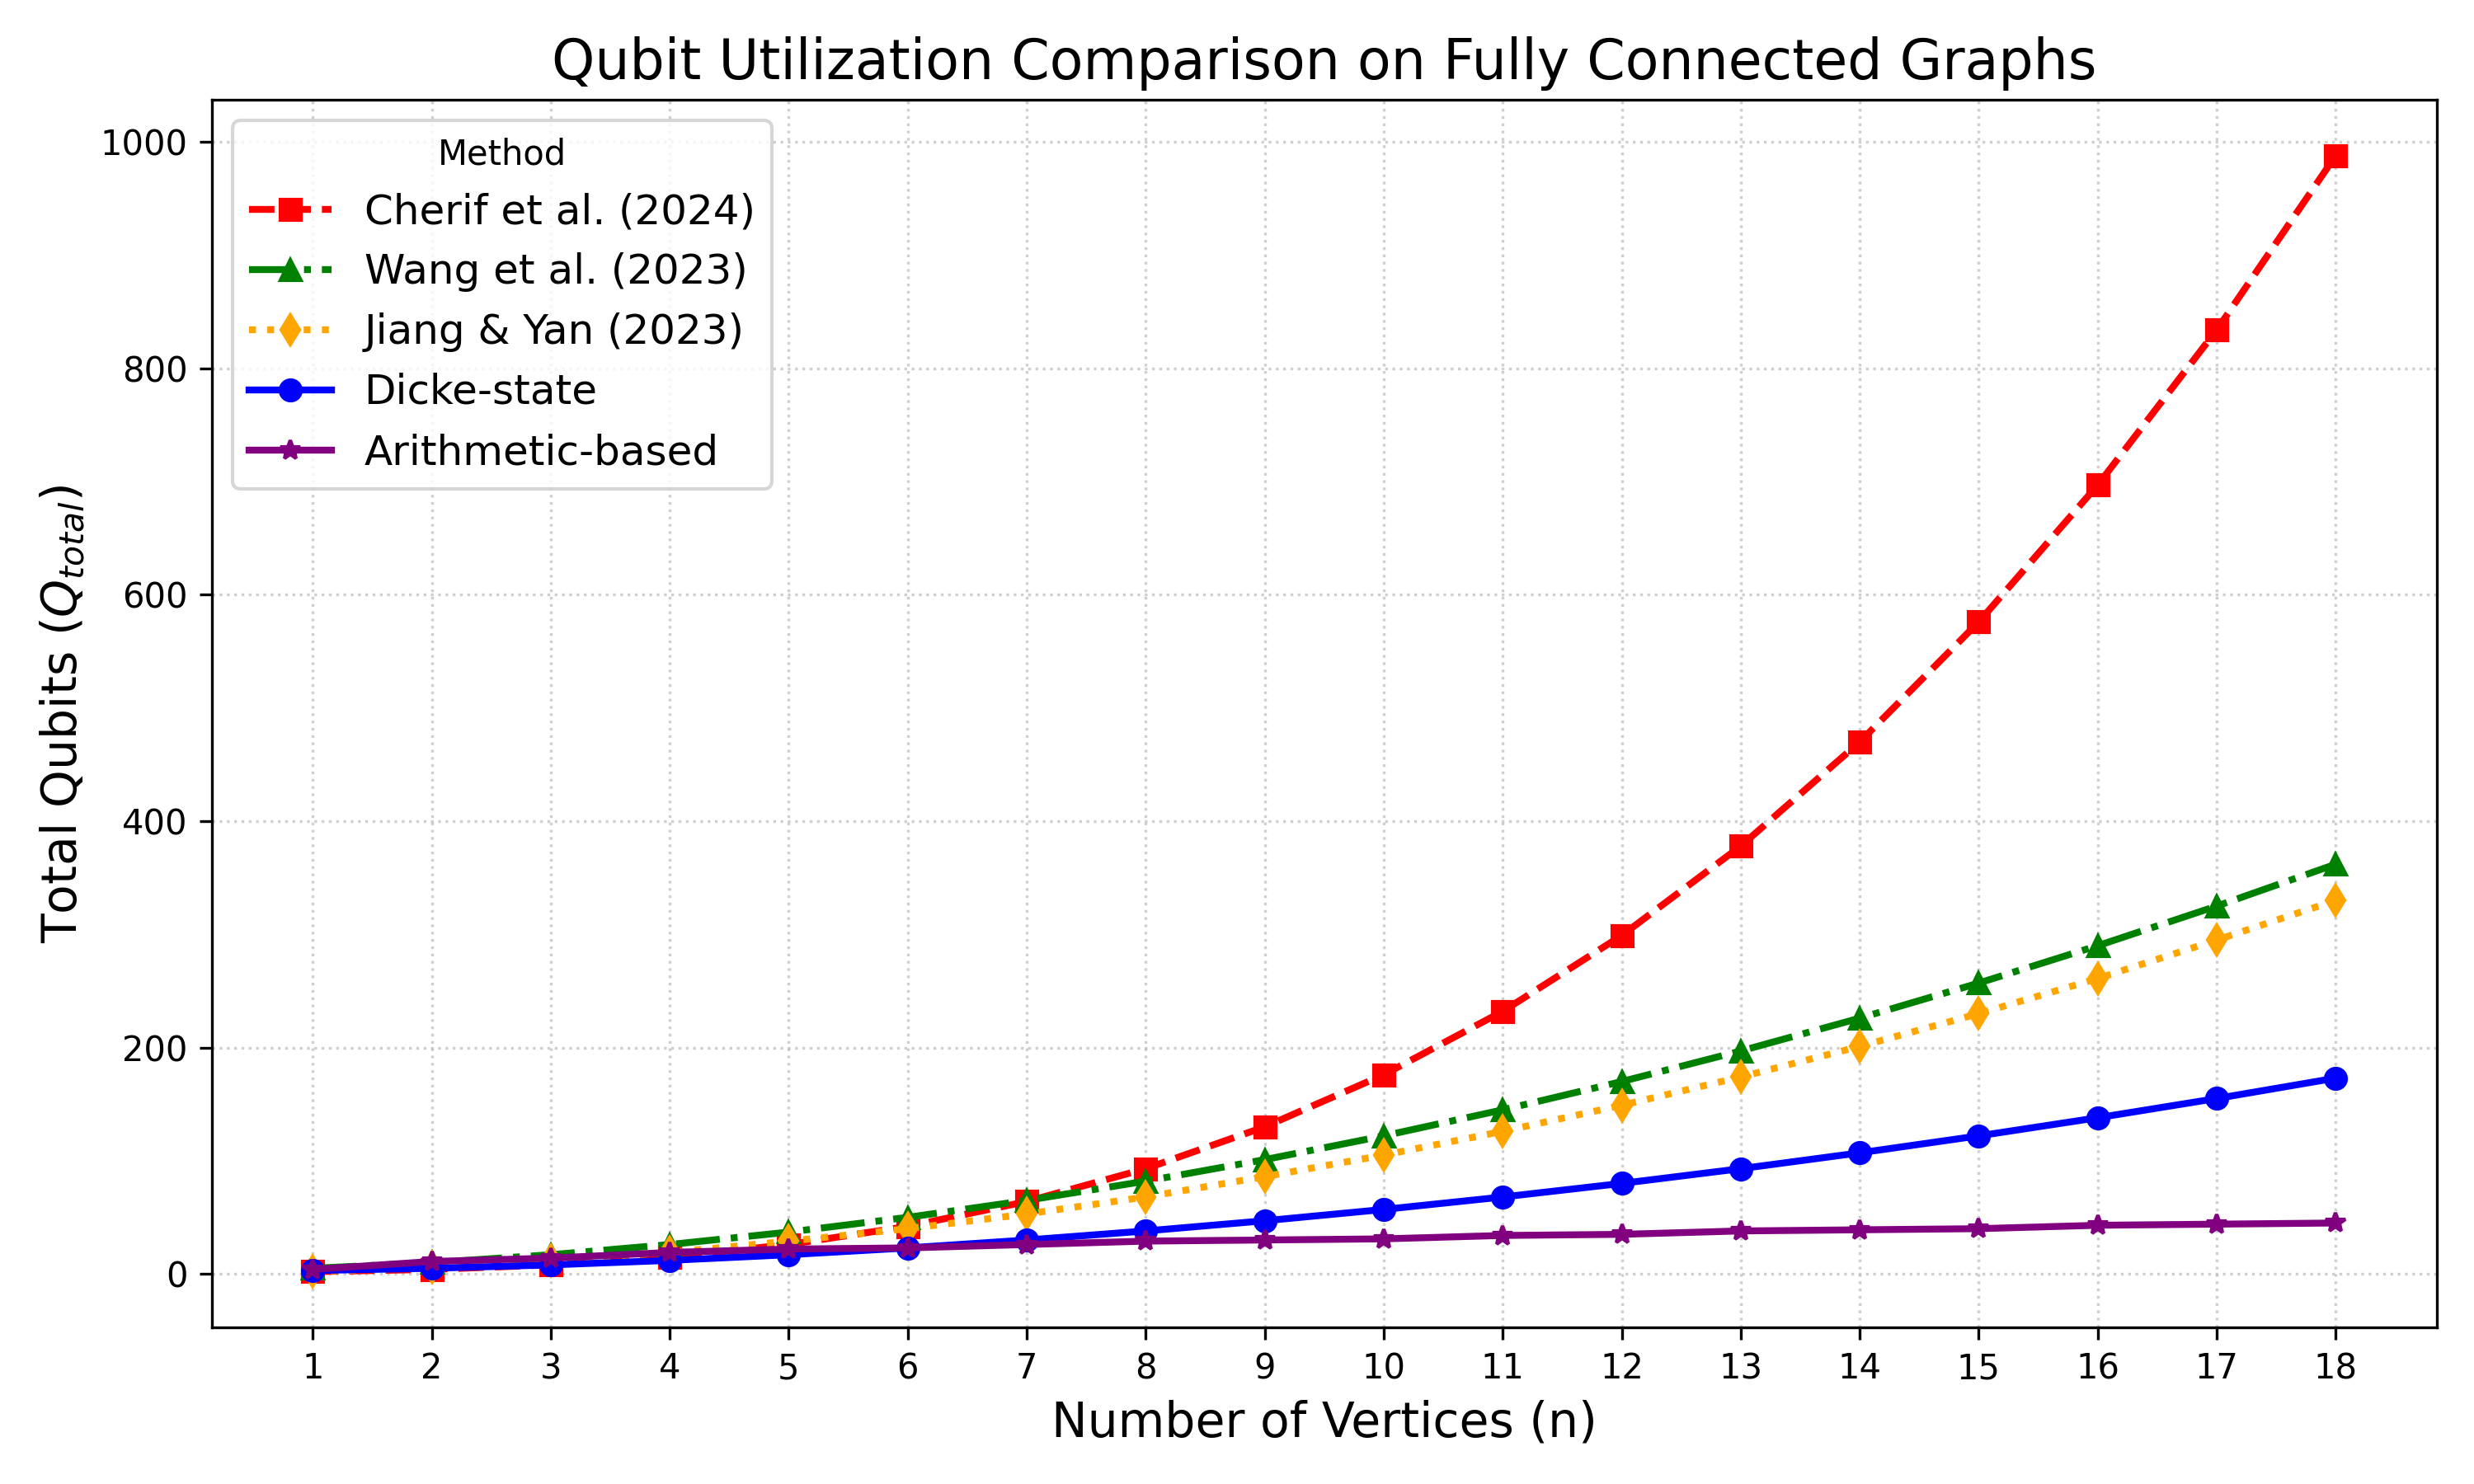
\includegraphics[width=\columnwidth]{figures/chart_qubit_scaling_comparison.png}
\caption{Qubit scaling comparison between proposed and prior work architectures on complete graphs for increasing graph size $n$.\label{fig:scaling}}
\end{figure}

However, this reduction in spatial resources introduces a trade-off in temporal resources (circuit depth). Table \ref{tab:depth_scaling} and Fig. \ref{fig:depth_scaling} compare the circuit depth per Grover iteration. The arithmetic oracles require sequential penalty additions and carry propagation, leading to a higher polylogarithmic depth overhead compared to the relatively shallow multi-controlled gate structure of the Dicke-state approach.

\begin{table}[htbp]
\caption{Circuit Depth Scaling Comparison per Grover Iteration}
\label{tab:depth_scaling}
\centering
\resizebox{\columnwidth}{!}{%
\begin{tabular}{|l|l|}
\hline
\textbf{Architecture} & \textbf{Per-Iteration Depth ($D_{iter}$)} \\
\hline
Cherif et al. (2024) & $O(m + \binom{n}{k+1})$ \\
Wang et al. (2023) & $O(n^2)$ \\
Jiang \& Yan (2023) & $O(n \log n + m)$ \\
Dicke-state (Ours) & $O(nk^2 + m)$ \\
Arithmetic-based (Ours) & $O(m \cdot \log n \cdot \log^2(nm))$ \\
Weighted (Ours) & $O((n + m \cdot \log(\sum w_i)) \cdot \log^2(nm))$ \\
\hline
\end{tabular}%
}
\end{table}

\begin{figure}[t!]
\centering
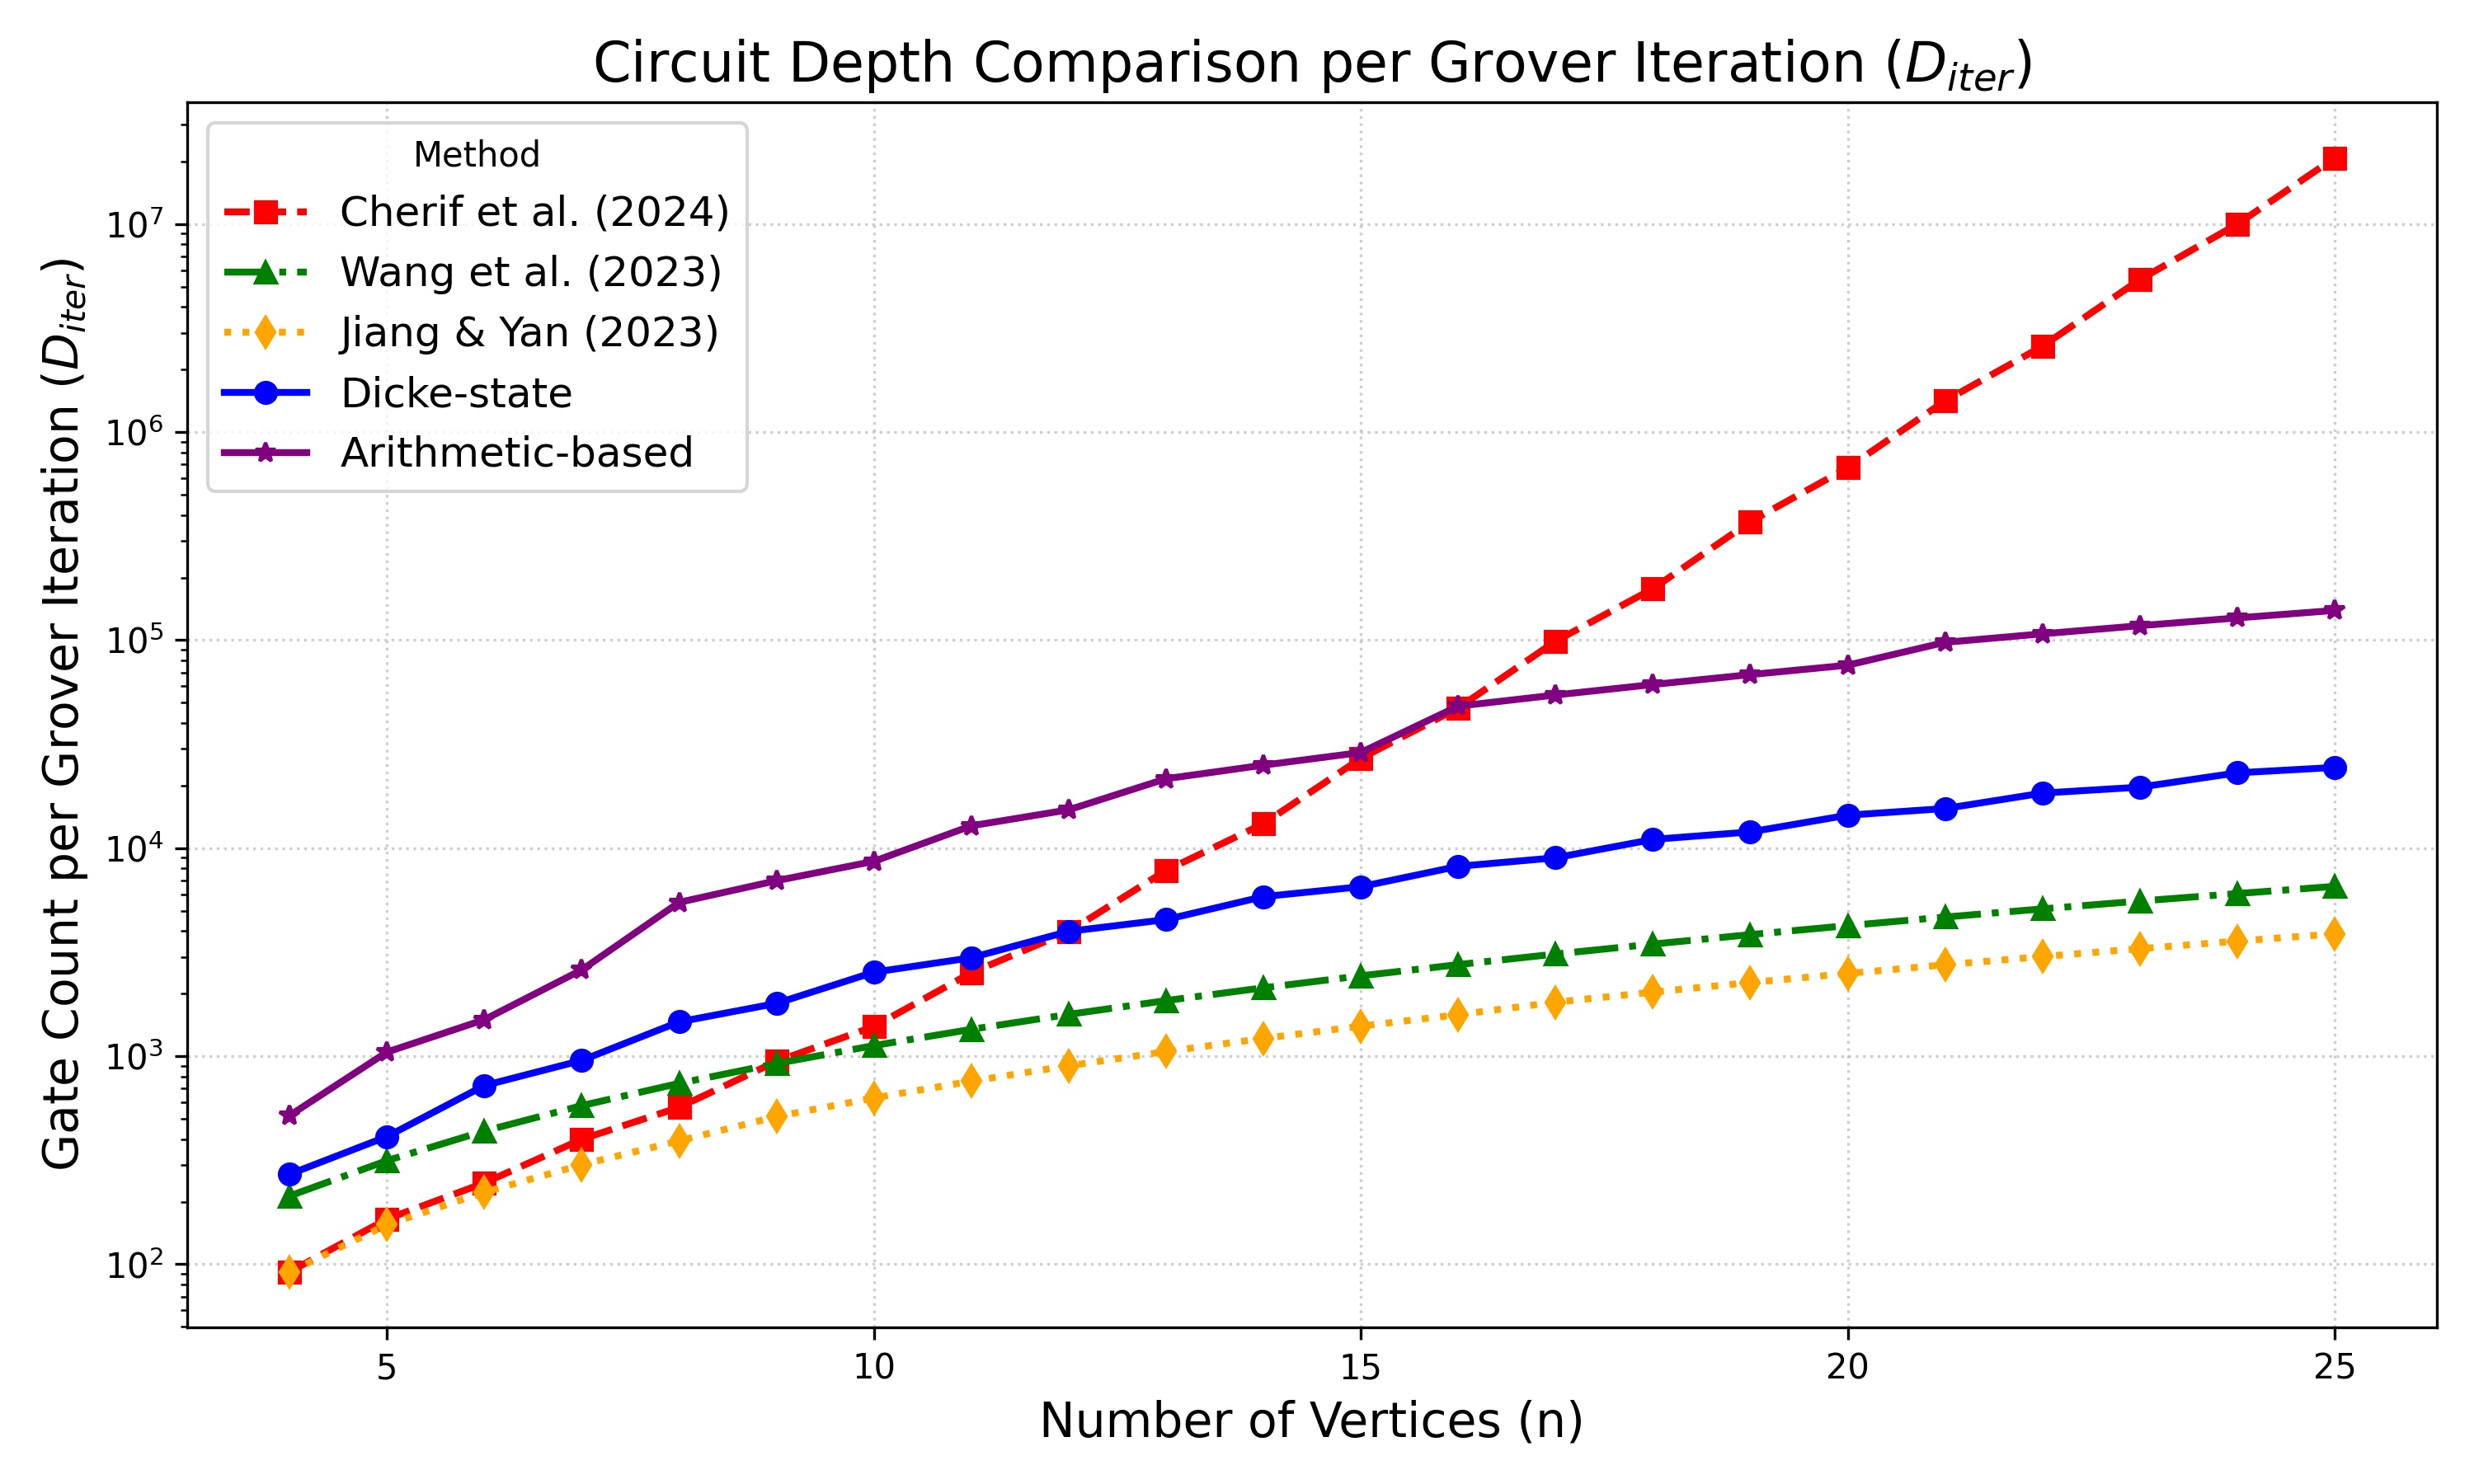
\includegraphics[width=\columnwidth]{figures/circuit_depth_comparison.png}
\caption{Circuit depth comparison per Grover iteration ($D_{iter}$) on complete graphs for increasing graph size $n$, comparing Dicke-state and Arithmetic-based architectures against prior works.\label{fig:depth_scaling}}
\end{figure}

\subsection{Circuit Architecture and Implementation}

\begin{figure}[t!]
\centering
\subfloat[$K_3$]{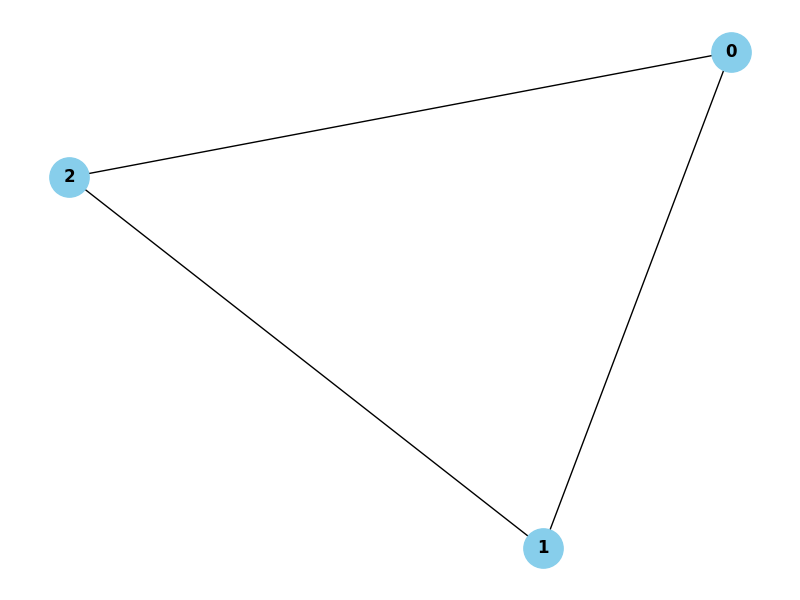
\includegraphics[width=0.15\textwidth]{figures/graph_K3_dicke_01.png}} \hfill
\subfloat[$C_4$]{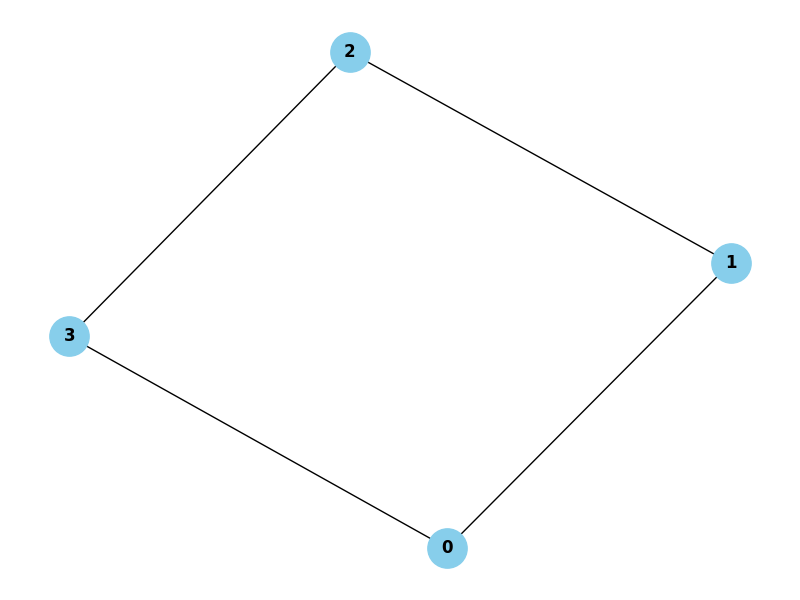
\includegraphics[width=0.15\textwidth]{figures/graph_cycle_C4_dicke_01.png}} \hfill
\subfloat[$C_5$]{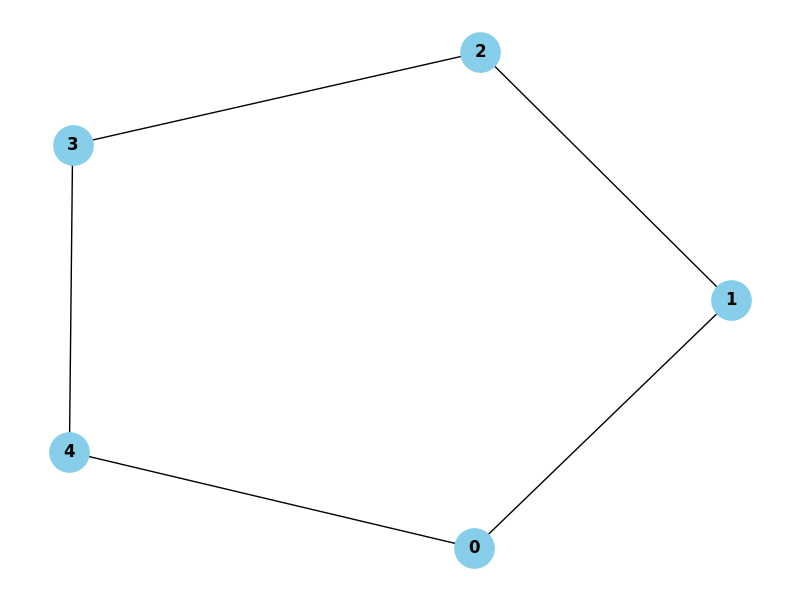
\includegraphics[width=0.15\textwidth]{figures/graph_cycle_C5_dicke_01.png}} \hfill
\subfloat[$C_6$]{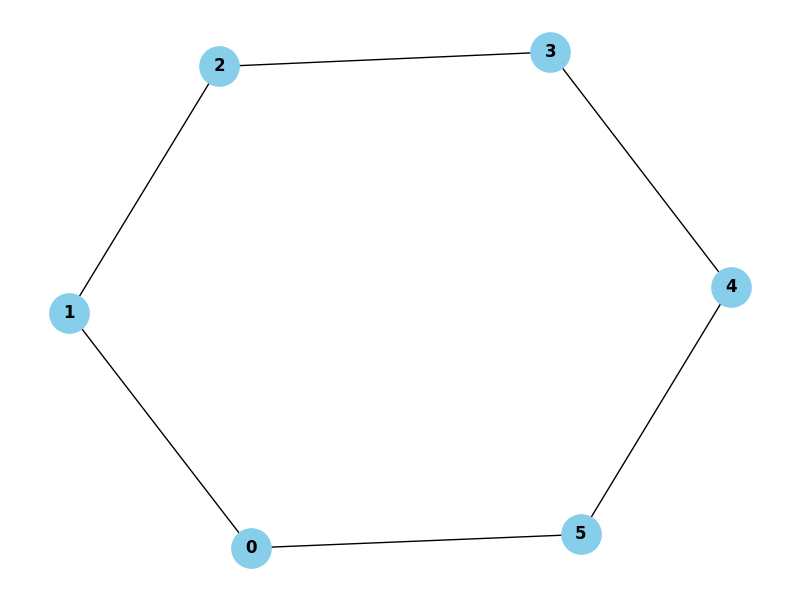
\includegraphics[width=0.15\textwidth]{figures/graph_cycle_C6_dicke_01.png}} \hfill
\subfloat[$K_6$]{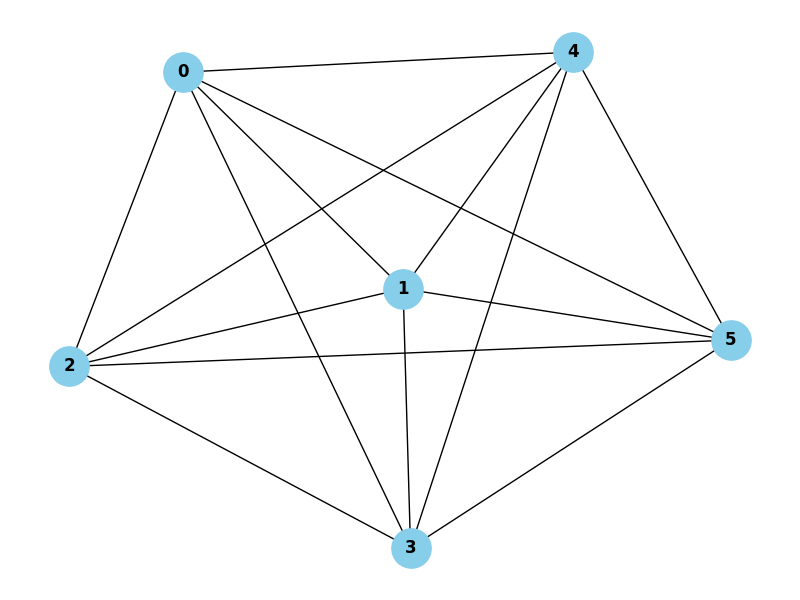
\includegraphics[width=0.15\textwidth]{figures/graph_K6_dicke_01.png}}
\caption{Benchmark graph visualizations used for performance evaluation.}
\label{fig:benchmark_graphs}
\end{figure}

The physical implementation of the Grover oracles fundamentally differs between the architectures. Fig. \ref{fig:circuit_comparison} illustrates the synthesized circuit diagrams for a 3-vertex complete graph ($K_3$). The Dicke-state architecture utilizes a parallel structure with $O(m)$ ancilla qubits, whereas the arithmetic architecture uses a sequential penalty addition approach to maintain the $O(\log m)$ ancilla footprint.

\begin{figure*}[t!]
\centering
\begin{minipage}{0.48\textwidth}
    \centering
    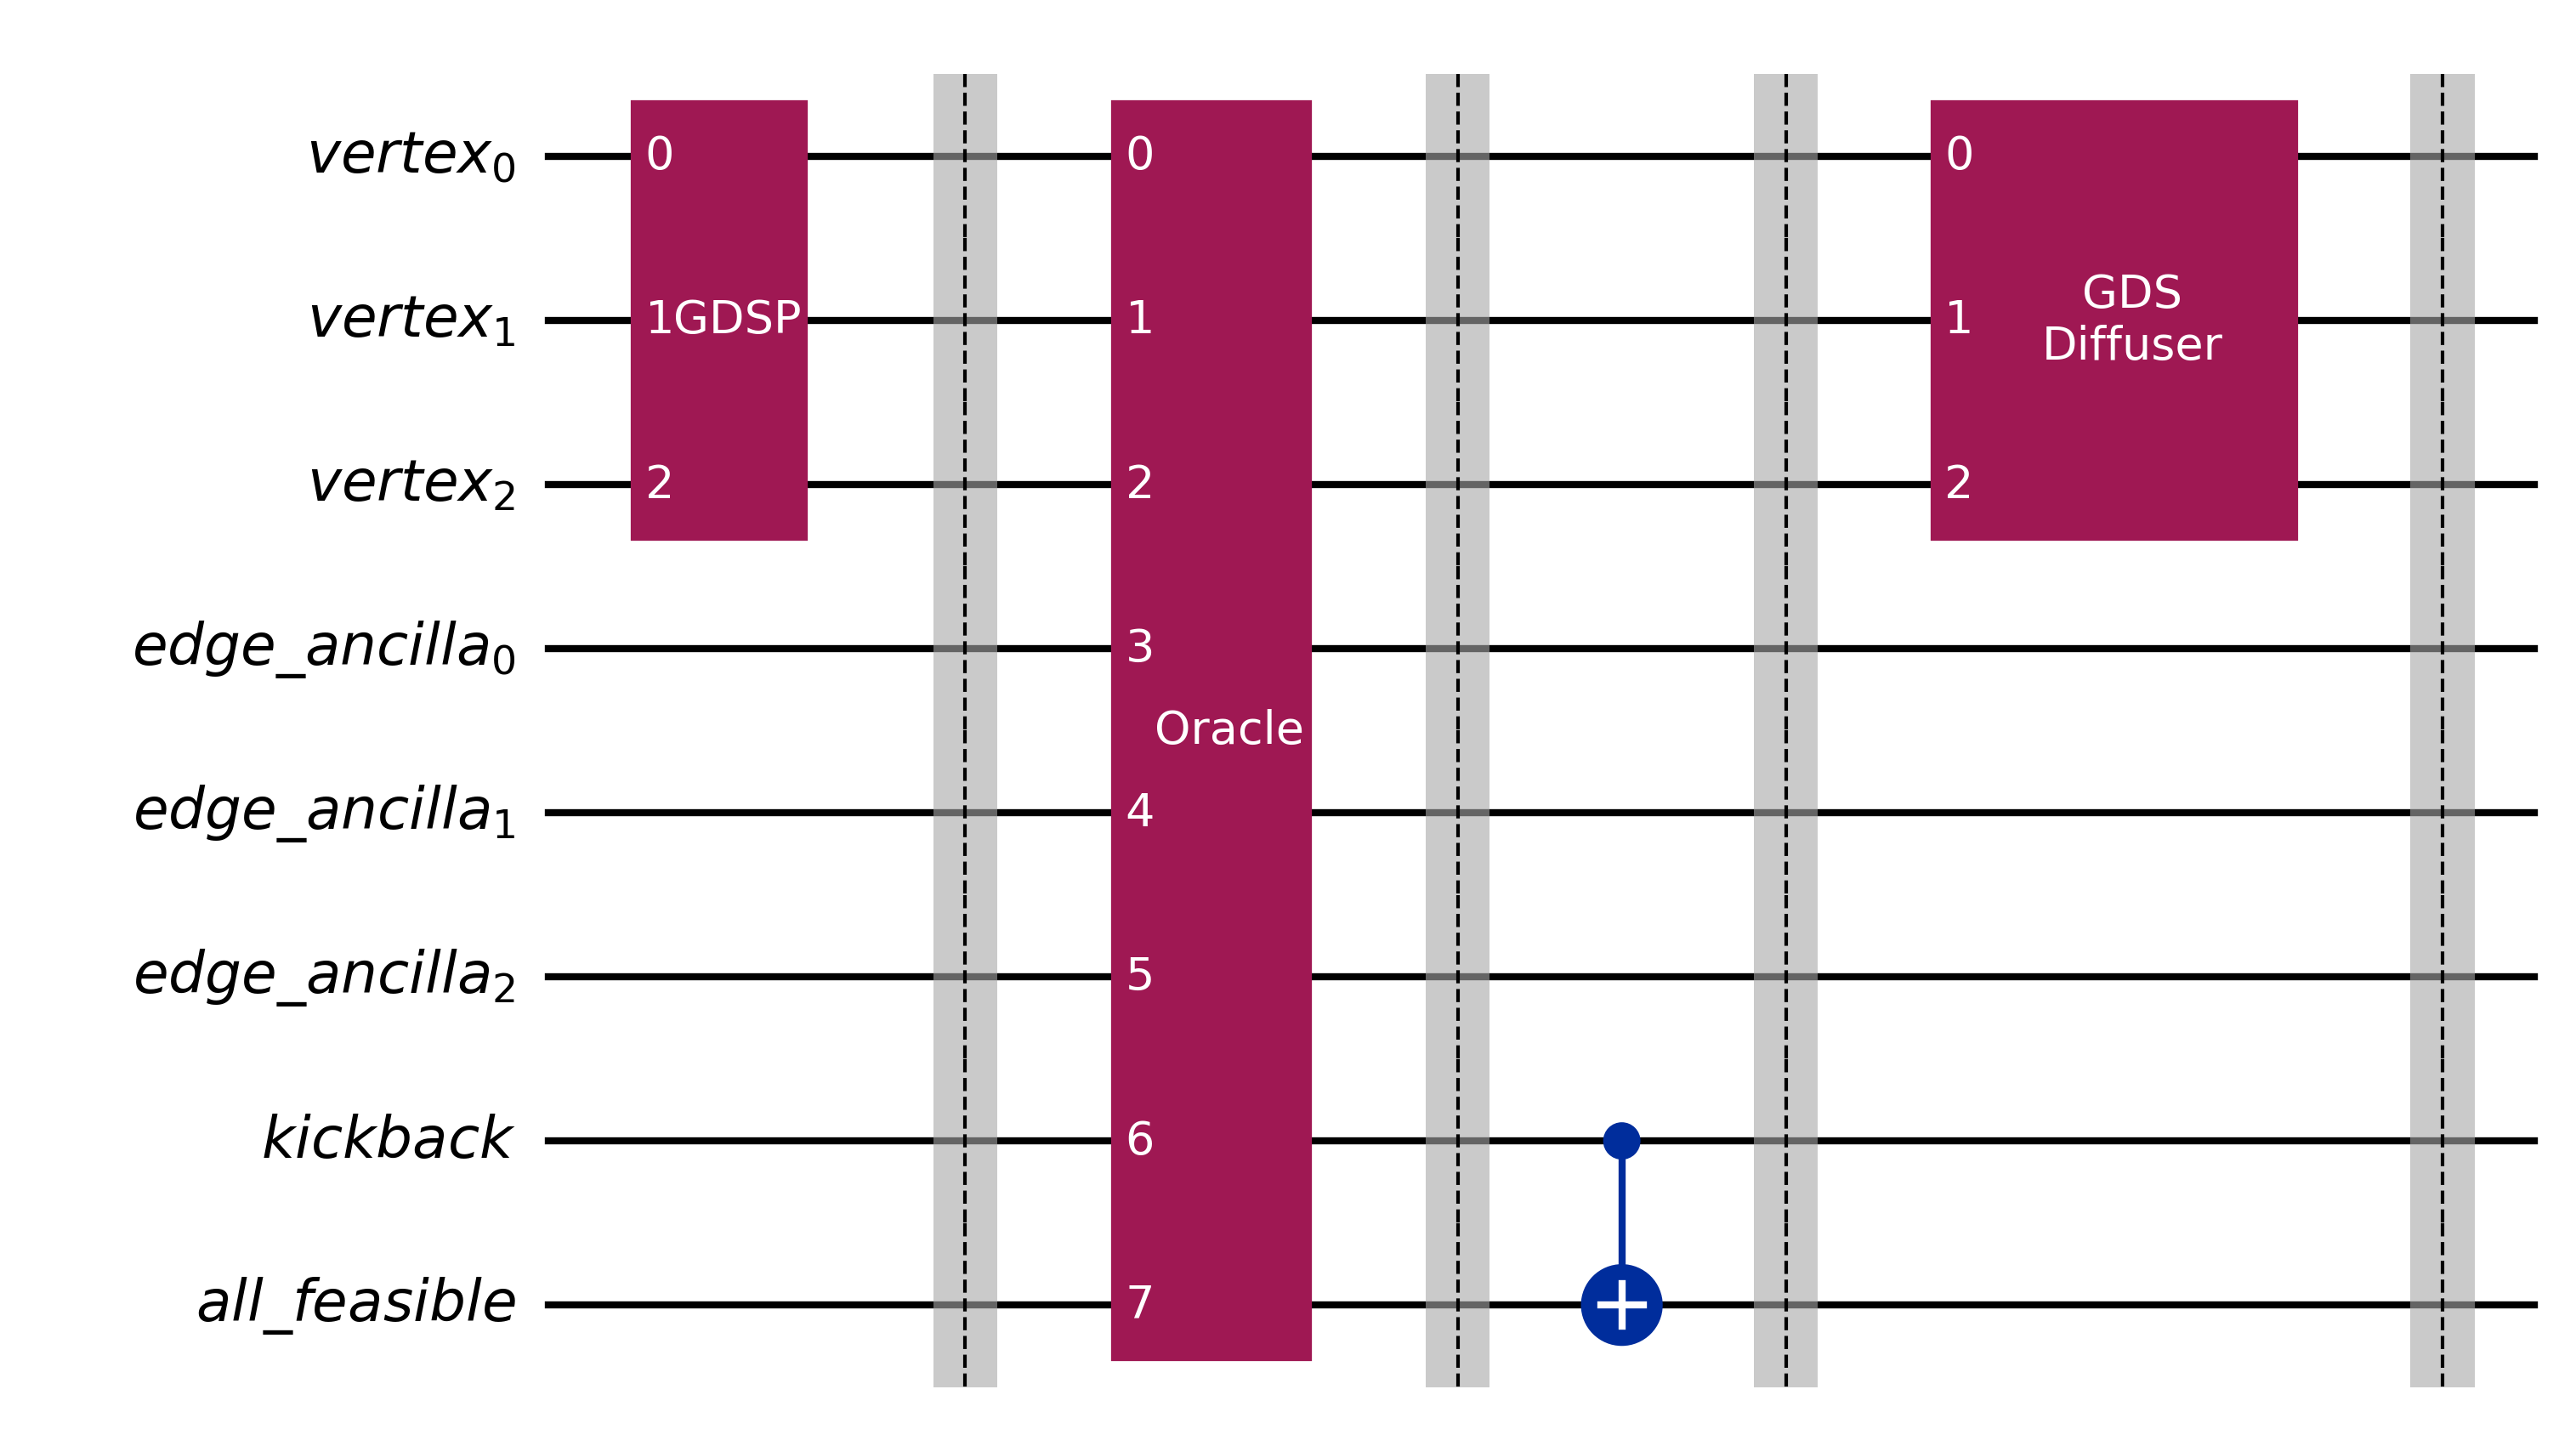
\includegraphics[width=\linewidth,keepaspectratio]{figures/circuit_K3_hierarchical_dicke_01.png}
    \caption*{(a) Dicke-state architecture ($K_3$)}
\end{minipage}
\hfill
\begin{minipage}{0.48\textwidth}
    \centering
    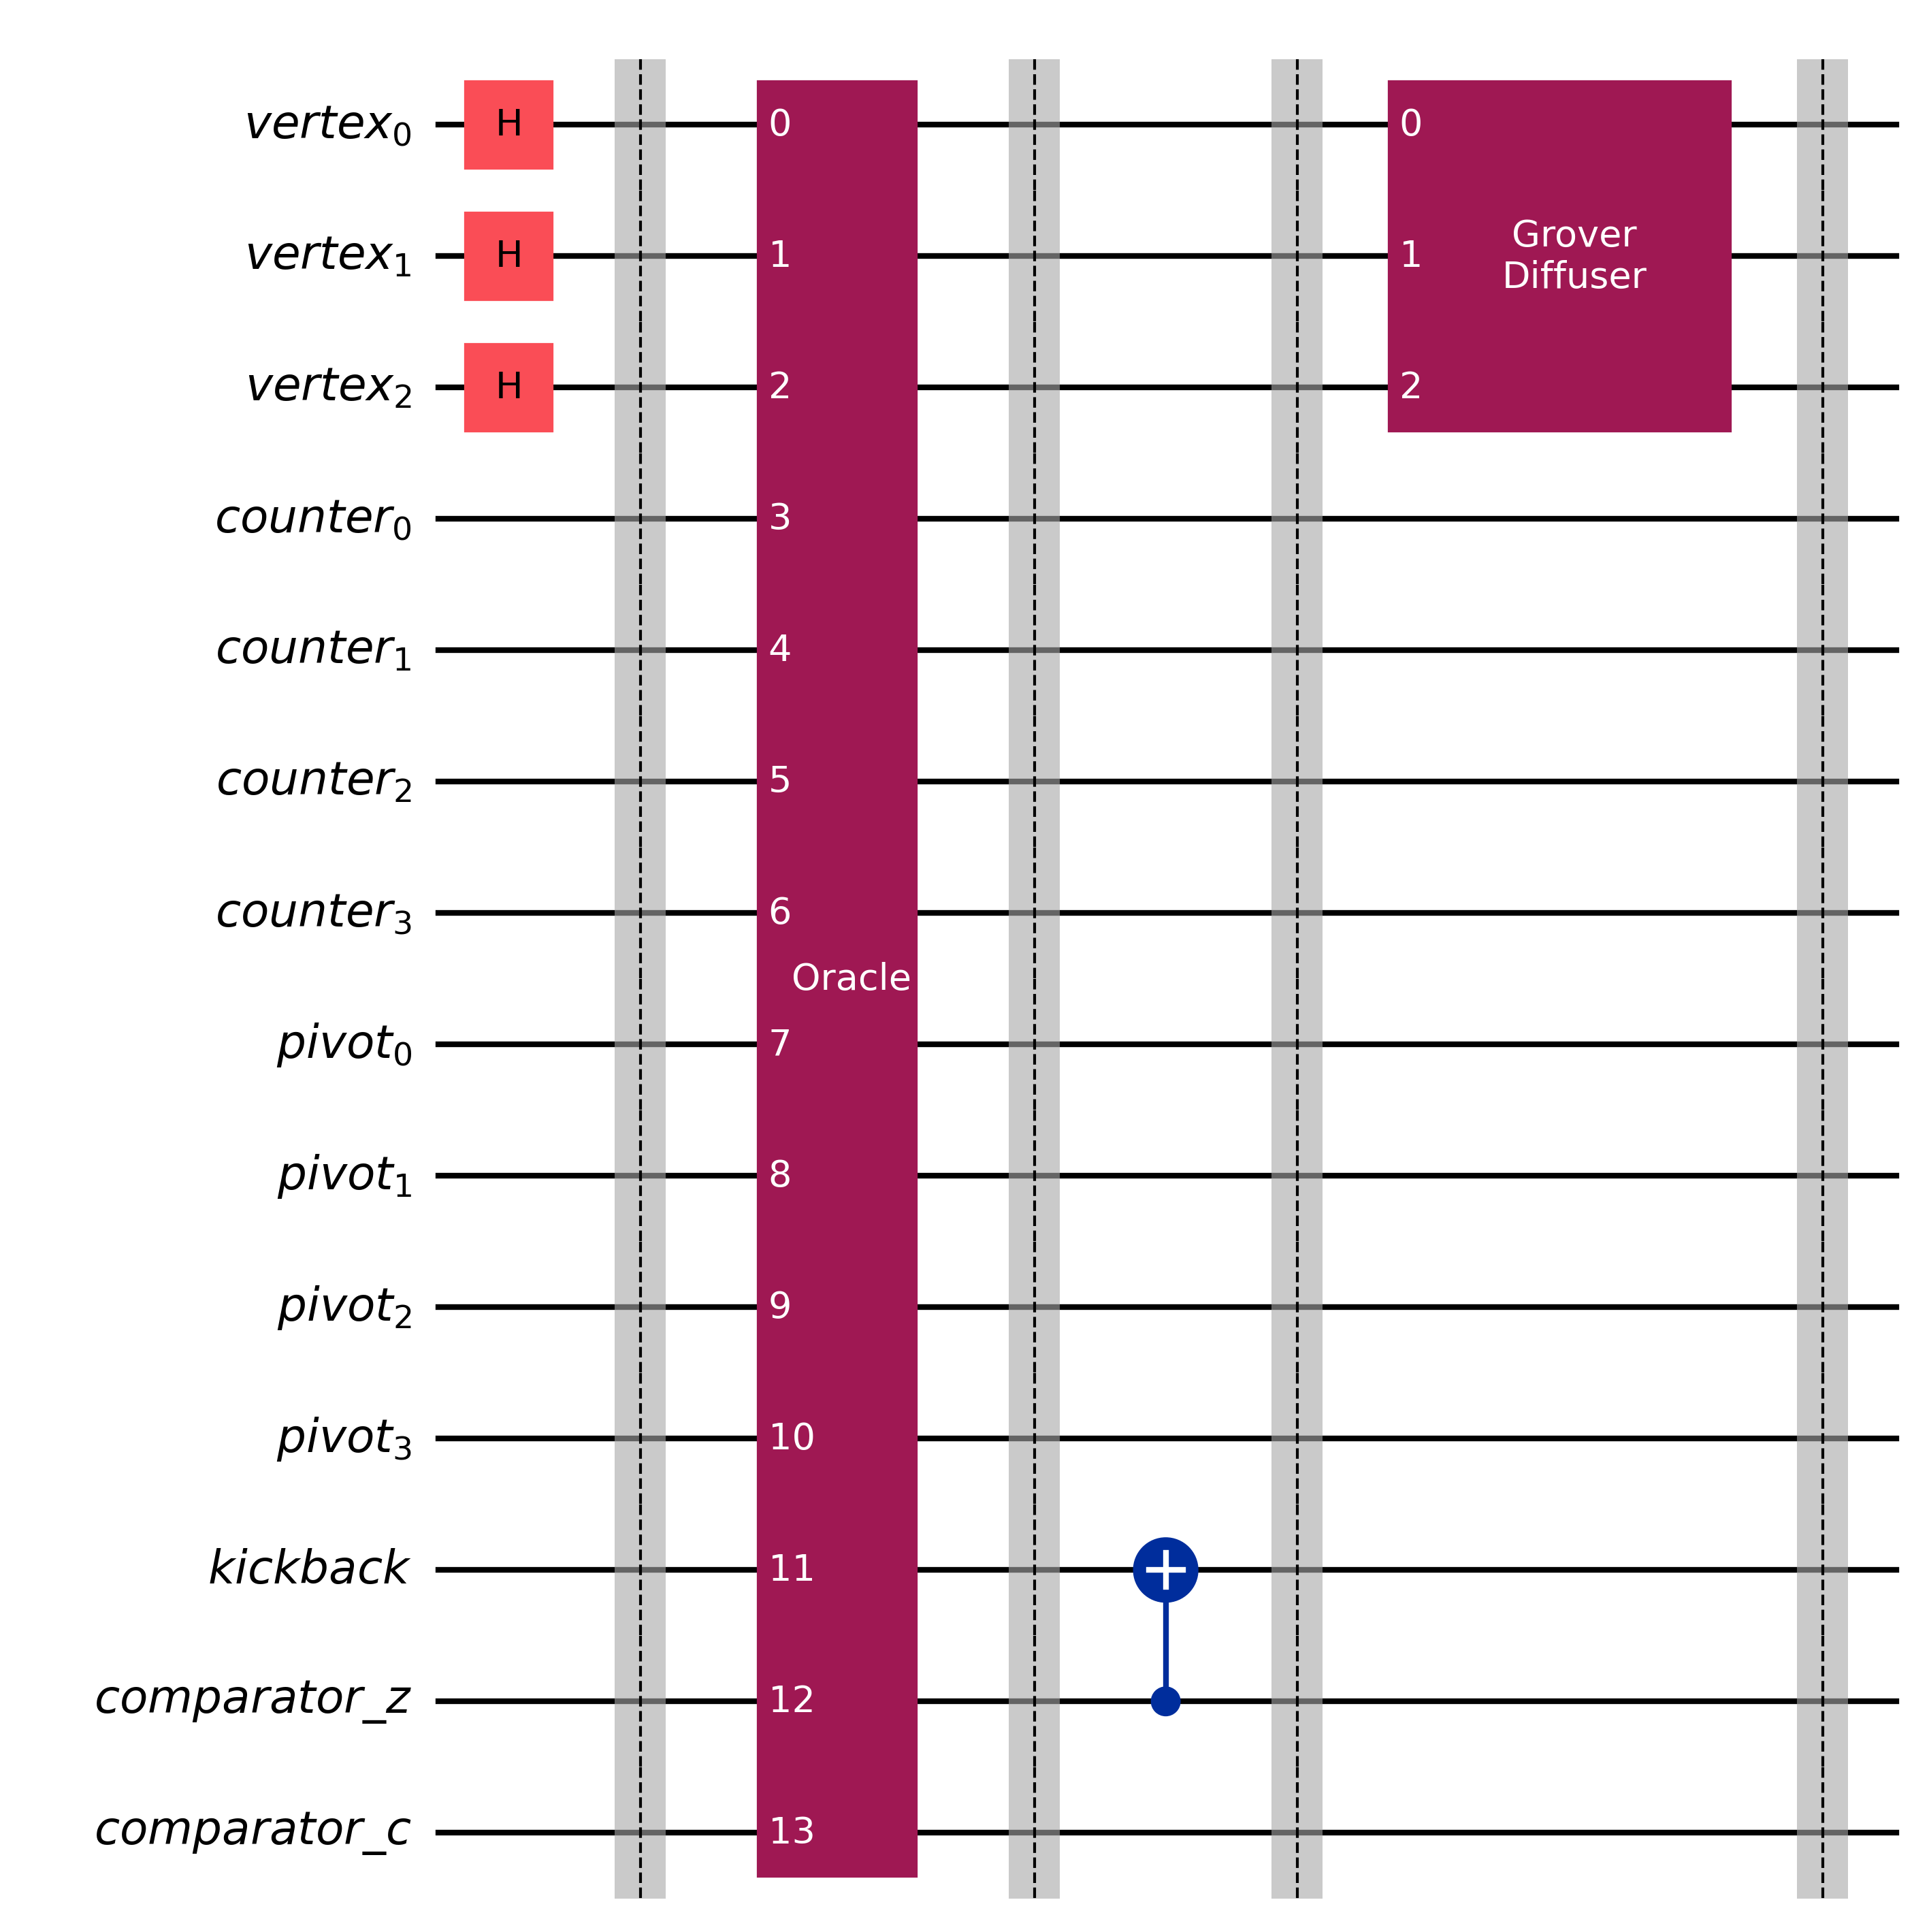
\includegraphics[width=\linewidth,keepaspectratio]{figures/circuit_K3_hierarchical_arith_01.png}
    \caption*{(b) Arithmetic architecture ($K_3$)}
\end{minipage}
\caption{Quantum circuit architecture comparison for an unweighted $K_3$ problem instance. (a) The Dicke-state oracle with the Edge Check component defined in detail in Fig. \ref{fig:edge_check_dicke}. (b) The arithmetic oracle with Popcount and Penalty Adder components defined in detail in Fig. \ref{fig:popcount_arith} and Fig. \ref{fig:penalty_arith}, respectively.}
\label{fig:circuit_comparison}
\end{figure*}

Furthermore, the weighted arithmetic solver successfully implements heterogeneous weight addition logic, where each vertex qubit controls the addition of its specific weight into the counter register via a binary-decomposed controlled-increment circuit.

To illustrate the qubit scaling advantage of our architectures, Fig. \ref{fig:k7_scaling} presents the circuit diagrams for a $K_7$ complete graph (7 vertices, 21 edges) using both Dicke-state and arithmetic architectures. The Dicke-state architecture requires 30 qubits (7 vertex + 21 edge ancillas + 2), while the arithmetic architecture requires only 26 qubits (7 vertex + 8 counter + 8 pivot + 3 ancilla), demonstrating the $O(\log m)$ ancilla efficiency for dense graphs.

\begin{figure*}[t!]
\centering
\begin{minipage}{0.45\textwidth}
    \centering
    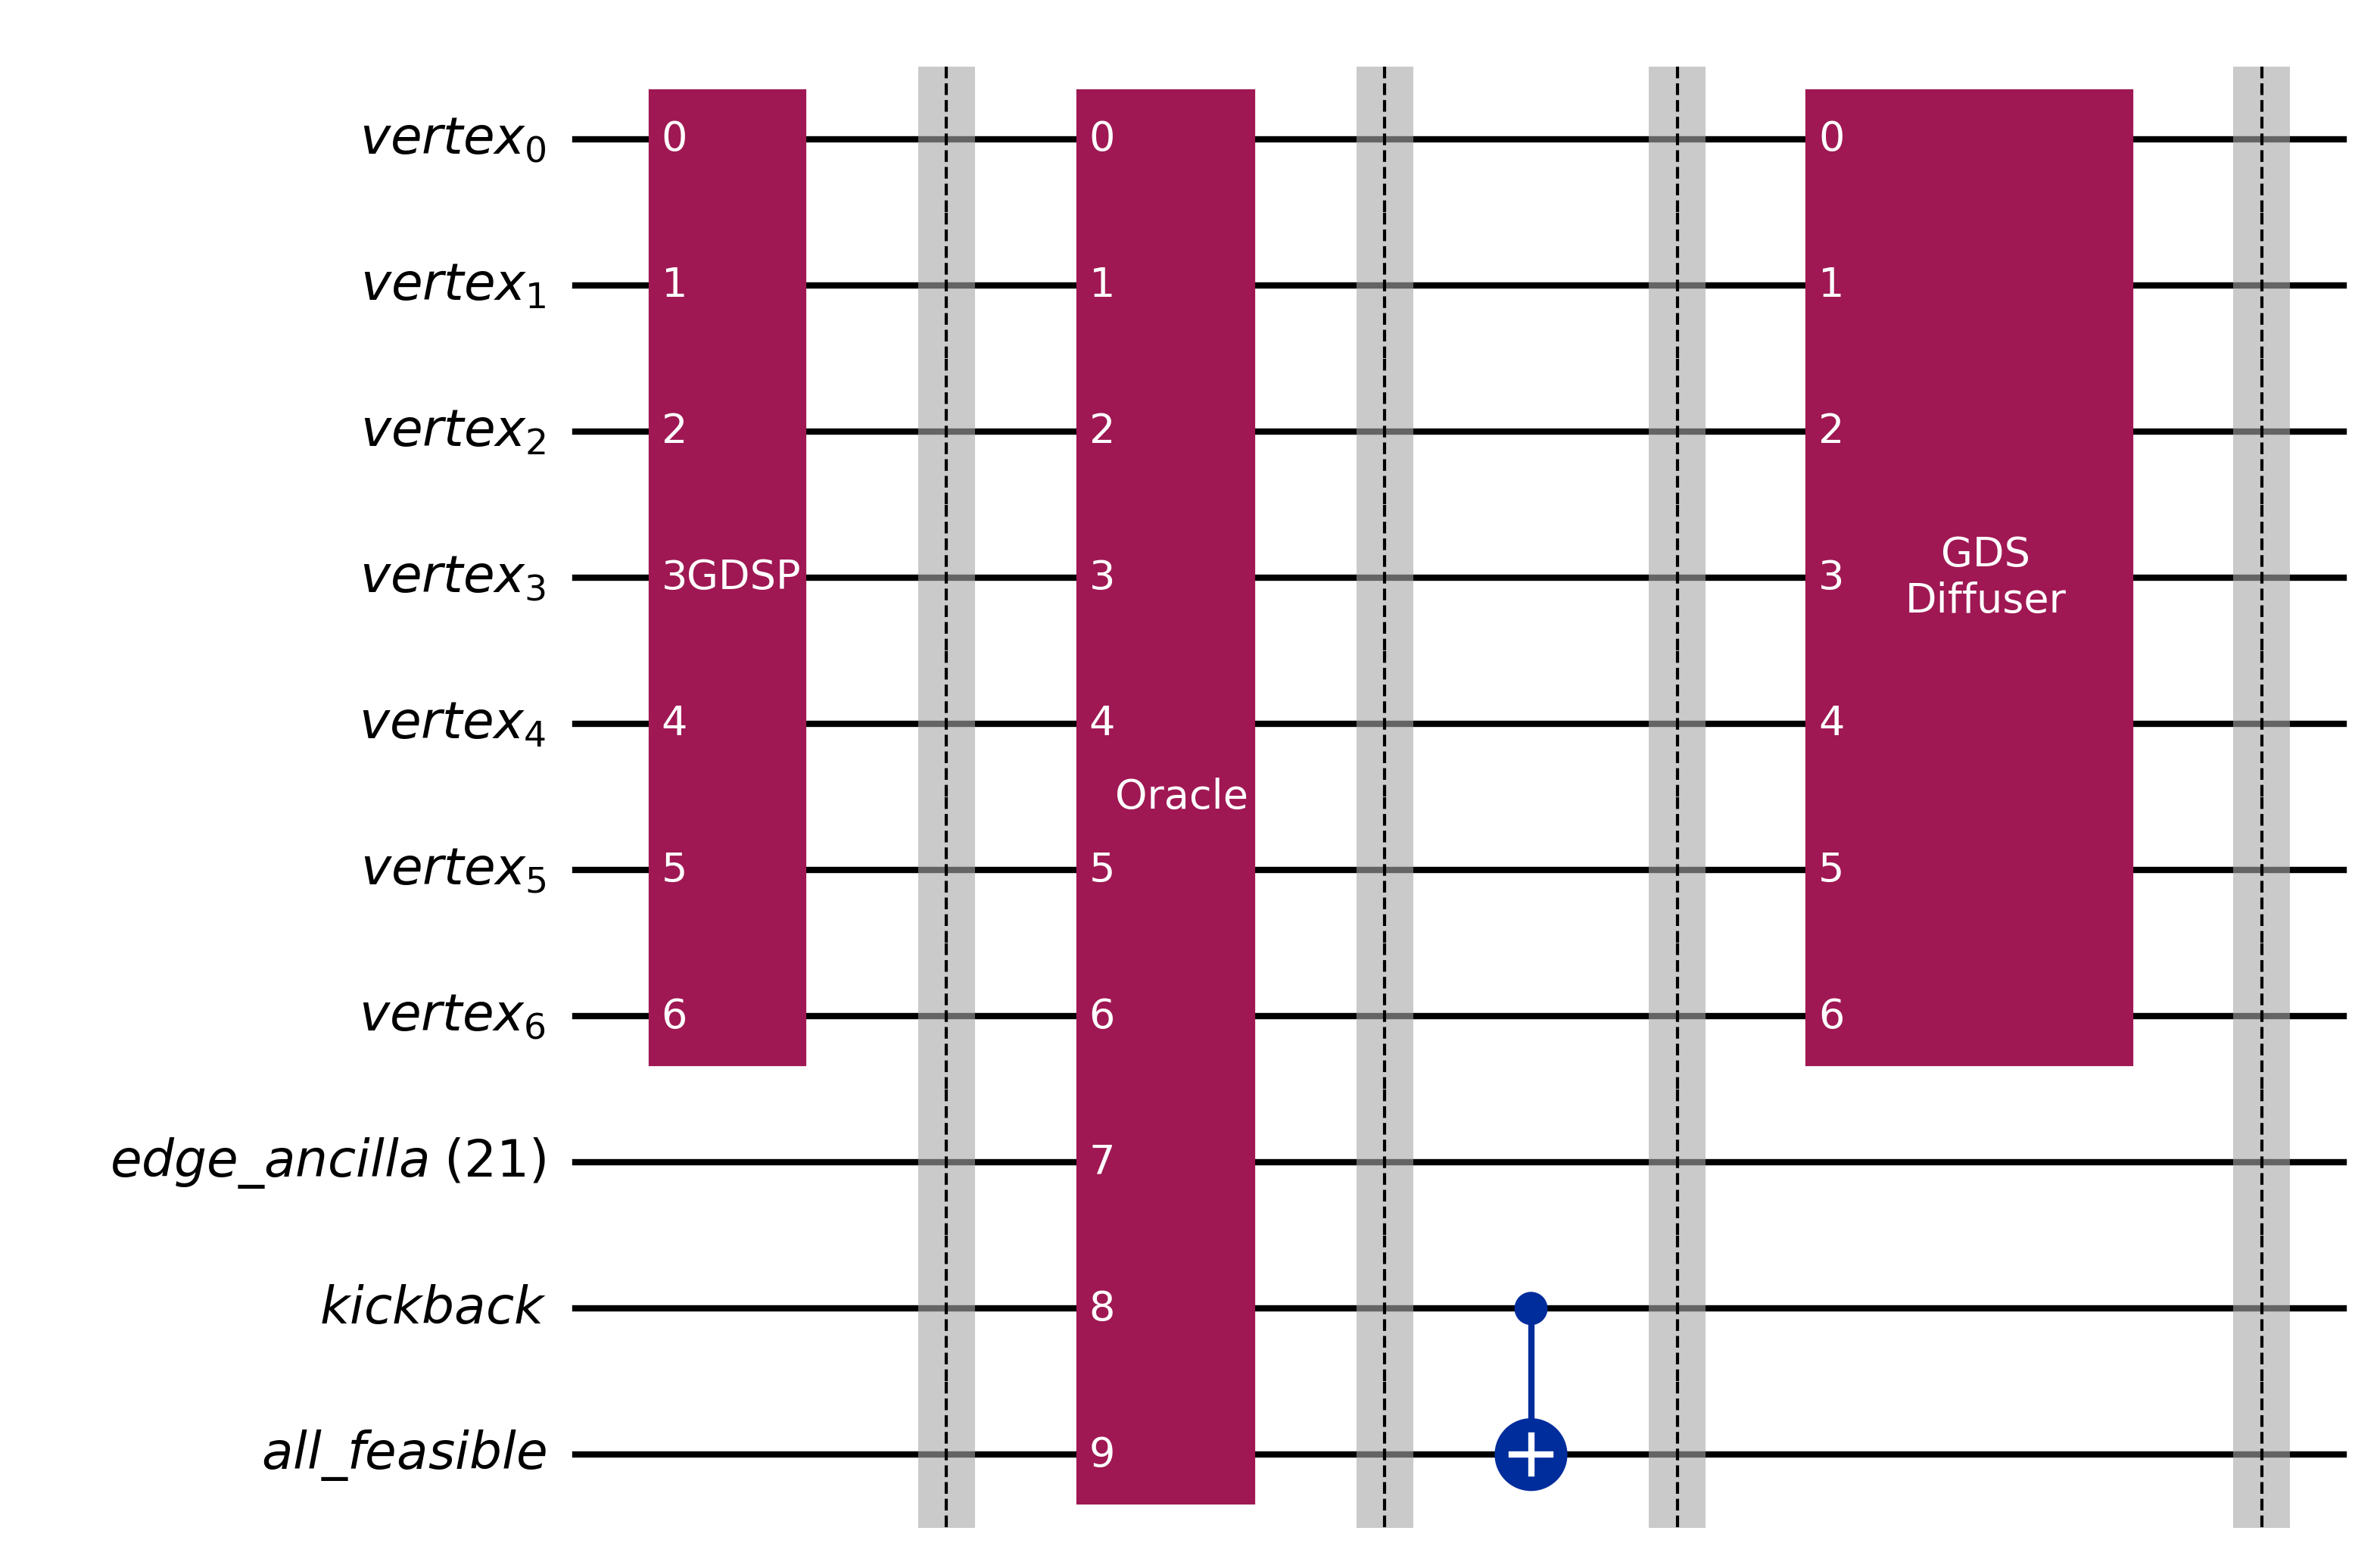
\includegraphics[width=\linewidth,keepaspectratio]{figures/circuit_K7_compact_dicke_01.png}
    \caption*{(a) Dicke-state architecture ($K_7$)}
\end{minipage}
\hfill
\begin{minipage}{0.45\textwidth}
    \centering
    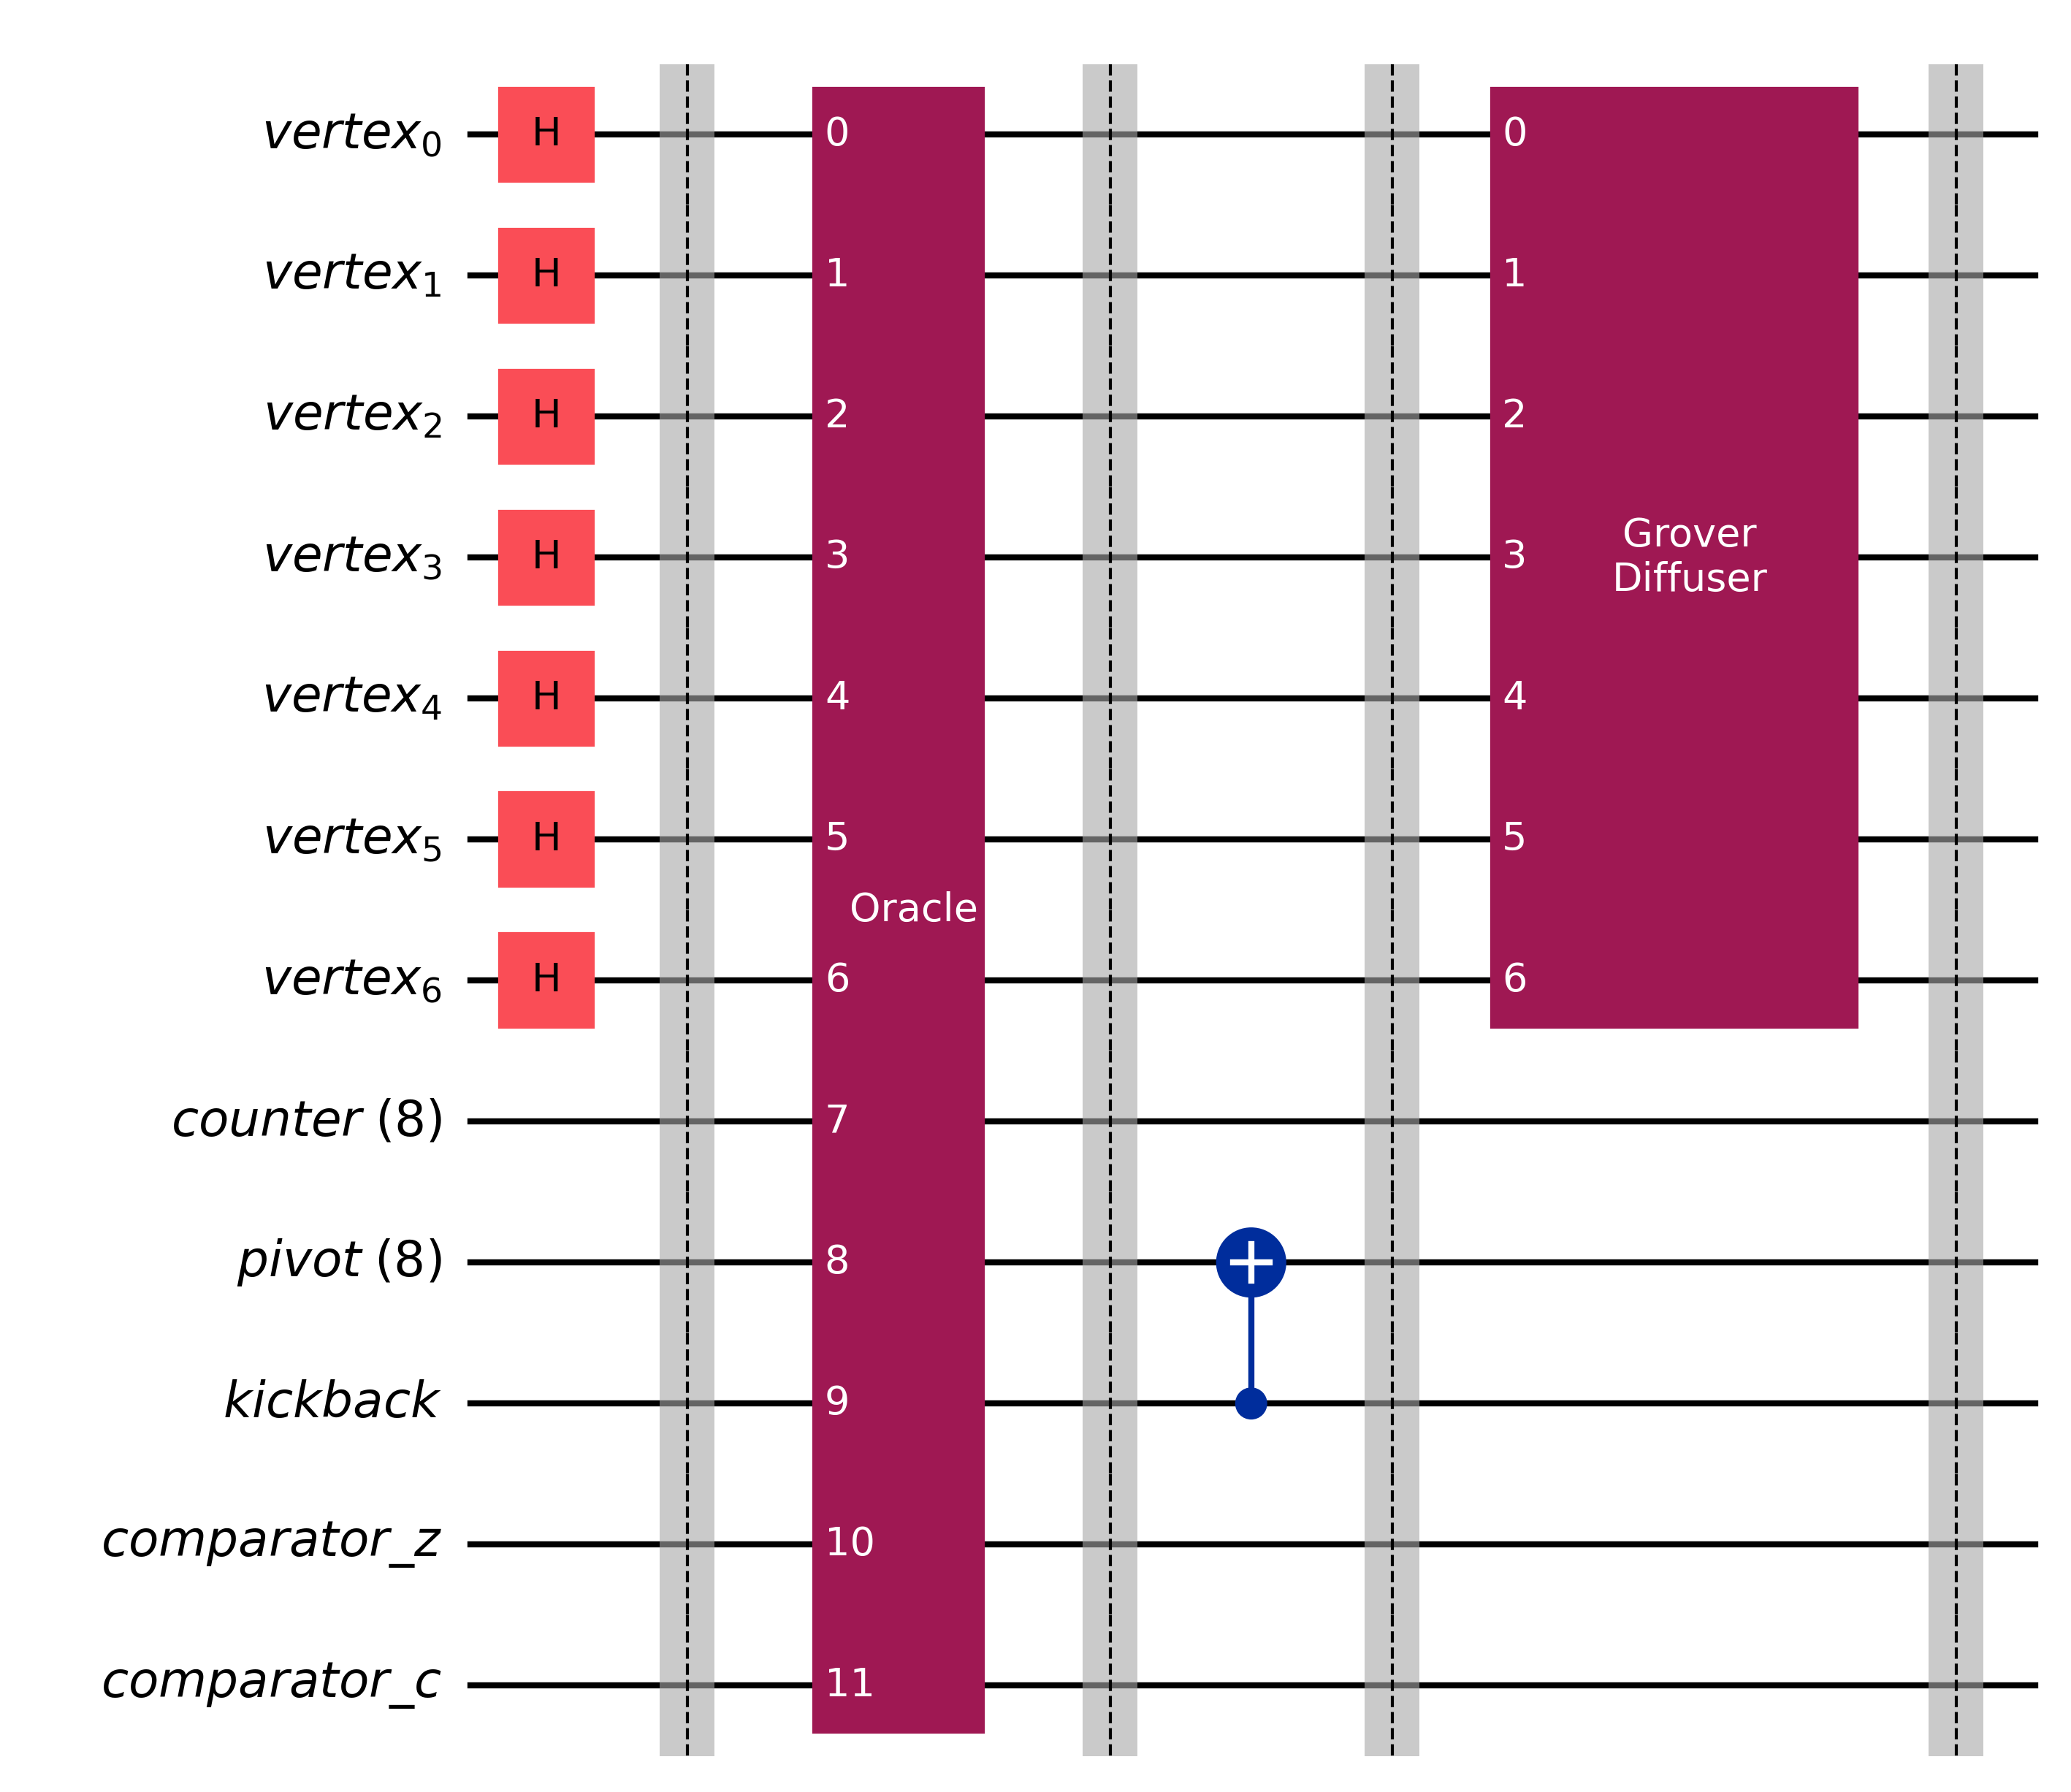
\includegraphics[width=\linewidth,keepaspectratio]{figures/circuit_K7_compact_arith_01.png}
    \caption*{(b) Arithmetic architecture ($K_7$)}
\end{minipage}
\caption{Qubit scaling comparison for $K_7$ (7 vertices, 21 edges). (a) Dicke-state oracle with Edge Check component defined in detail in Fig. \ref{fig:edge_check_dicke}. (b) Arithmetic oracle with Popcount and Penalty Adder components defined in detail in Fig. \ref{fig:popcount_arith} and Fig. \ref{fig:penalty_arith}, respectively. The compact view groups registers for clarity.}
\label{fig:k7_scaling}
\end{figure*}

\subsection{Simulation Performance}


To validate our theoretical designs, we conducted state-vector simulations on a set of benchmark graphs, shown in Fig. \ref{fig:benchmark_graphs}. These include dense structures (complete graphs $K_n$) and sparse, symmetric structures (cycle graphs $C_n$).


Fig. \ref{fig:k3_comparison} (see Appendix) displays the solution probability distributions for $K_3$ (MVC=2) with pivot=3. Both approaches successfully amplify valid vertex covers. Notably, the Dicke-state architecture exhibits exactly zero probability for states with Hamming weight $> 3$ due to the rigorous initial state filtering, whereas the arithmetic architecture distributes minor residual probabilities across the full $2^n$ space but still distinctly peaks at the valid solutions.

Scaling to larger complete graphs, Fig. \ref{fig:k4_comparison} (see Appendix) shows results for $K_4$ (MVC=3, pivot=4), while Fig. \ref{fig:k5_comparison} (see Appendix) depicts $K_5$ (MVC=4, pivot=5).

The empirical limits of classical state-vector simulation are demonstrated in Fig. \ref{fig:k6_comparison} (see Appendix) ($K_6$, MVC=5, pivot=6). Fig. \ref{fig:k7_comparison} (see Appendix) shows the $K_7$ result (MVC=6, pivot=7) using the arithmetic architecture, which required 26 qubits, representing the memory capacity upper bound of our classical backend.

Performance on sparse cycle graphs ($C_4, C_5, C_6$) using both Dicke-state and arithmetic architectures is validated in Fig. \ref{fig:c4_comparison}, Fig. \ref{fig:c5_comparison}, and Fig. \ref{fig:c6_comparison} (see Appendix). Both architectures consistently identify the minimum cardinality cover within minimal Grover iterations.

Finally, for the Weighted MVC problem, we evaluate three diverse cost topologies: $K_3$ with weights (1,2,3), a path graph $P_4$ with weights (1,2,3,4), and a star graph $S_4$ with extreme heterogeneous weights (1,1,10,10) (see Fig. \ref{fig:weighted_graph} in Appendix). The solution distributions in Fig. \ref{fig:dist_weighted} (see Appendix) confirm the weighted arithmetic architecture's robust capability to isolate the lowest-cost vertex configurations regardless of the underlying graph topology.

Overall, the simulation results empirically confirm that all three architectures successfully identify minimum vertex covers. When the algorithmic pivot is set to the absolute minimum weight plus one (MVC+1), the quantum amplitude amplification correctly and exclusively marks solutions with weights strictly less than the pivot as valid states.

% ============================================================
% แทนที่ \subsection{QAOA Baseline Comparison} ทั้งหมด
% labels, \ref{}, \cite{} ทุกตัวคงเดิมจาก original
% ============================================================

\subsection{QAOA Baseline Comparison}
\label{sec:qaoa_comparison}

To contextualize our Grover architectures against the
dominant variational approach, we implemented a QAOA
benchmark suite using the standard MVC QUBO
formulation~\cite{farhi2014qaoa,pellow-jarman_qaoa_2024}.
For each graph, we map the QUBO to an Ising Hamiltonian,
optimize $p$-layer QAOA angles via SPSA with random
restarts (5 restarts, 80 iterations, 4096 shots per
evaluation), and simulate the final circuit on
AerSimulator with 4096 shots. We test $p \in \{1,2,3\}$.

% ------ resource disclaimer ------
\paragraph{Comparison Setting}
We emphasize that this comparison is conducted under a
\emph{resource-unconstrained} setting: QAOA uses only $n$
qubits regardless of $p$, whereas our Grover architectures
require $O(n+m)$ qubits (Dicke-state) or $O(n + \log m)$
qubits (arithmetic-based), as shown in
Fig.~\ref{fig:qaoa_qubits} and
Table~\ref{tab:qaoa_resources}. This comparison therefore
does not reflect a fair qubit-budget trade-off, but
evaluates each approach at its natural operating point.
The primary metric of interest is \emph{success
probability}, defined as the probability of measuring an
optimal solution in a single shot, since this directly
determines the number of circuit repetitions needed in
practice.

Tables~\ref{tab:qaoa_success} and~\ref{tab:qaoa_resources}
summarize the empirical results. While QAOA achieves an
approximation ratio of 1.0 on all instances, meaning the
\emph{best observed cost} equals the true minimum, this
metric obscures a critical limitation in the success
probability. Because the QUBO penalty term is ``soft''
(encoded as an energy offset rather than a hard
constraint), the cost gap between the optimal cover and
the all-1's state (selecting every vertex) is small.
Consequently, QAOA's mixer Hamiltonian populates
high-Hamming-weight states disproportionately.

For example, on $K_6$ with $p=1$, the suboptimal all-1's
state $|111111\rangle$ (cost $-84$) is measured with
$64.1\%$ probability, whereas the optimal states (size 5,
cost $-85$) collectively receive only $\approx 27.4\%$.
Similarly, on $K_7$ with $p=1$, the all-1's state
captures $47.7\%$ of the probability mass despite being
suboptimal, while the optimal states share only
$\approx 33.2\%$. This means that even though QAOA's
\emph{best} shot may be optimal, the overwhelming majority
of shots are wasted on unnecessarily large covers.

% ------ K3 exception explained ------
\paragraph{Small-Graph Regime ($n \leq 3$)}
An important exception occurs on $K_3$, where QAOA at
$p = 3$ achieves a success probability of 0.971, which
\emph{exceeds} both the arithmetic-based (0.858) and
Dicke-state (0.704) Grover architectures
(Table~\ref{tab:qaoa_success}). This result is expected
and consistent with the known behavior of QAOA on small
instances: for $n = 3$ the QUBO energy landscape contains
only $2^3 = 8$ states, and the cost gap between optimal
and suboptimal covers is large relative to the total
energy scale. In this regime, three QAOA layers suffice
to concentrate amplitude on the optimal manifold, and the
soft-penalty formulation does not yet suffer from the
high-Hamming-weight crowding that emerges at larger graph
sizes. The shallow transpiled depth of QAOA at $p=3$
(Table~\ref{tab:qaoa_resources}) also minimizes
decoherence, compounding its advantage on this small
instance.

% ------ Grover advantage framed correctly ------
\paragraph{Large-Graph Regime and Scaling Advantage}
The picture changes markedly as $n$ grows. As shown in
Fig.~\ref{fig:qaoa_success}, Grover achieves success
probabilities of $42\%$--$100\%$ (depending on graph size
and architecture), while QAOA's success probability
degrades to as low as $8\%$--$9\%$ at $p=2$ for dense
graphs (see SPSA convergence trajectories in Appendix
Figs.~\ref{fig:qaoa_conv_k3}--\ref{fig:qaoa_conv_k7}).
The critical pattern in Table~\ref{tab:qaoa_success} is
that \emph{QAOA's success probability degrades with graph
size while Grover's remains comparatively stable}. On
$K_6$, QAOA drops to 0.274 ($p=1$) and 0.090 ($p=2$),
whereas our arithmetic-based and Dicke-state architectures
maintain 0.644 and 0.649 respectively. On $K_7$, QAOA at
$p=2$ collapses to 0.084, while the arithmetic
architecture retains 0.420.

This degradation arises from two compounding effects.
First, the soft QUBO penalty term causes the energy gap
between optimal and suboptimal covers to shrink relative
to the total energy scale as $n$ grows, making the QAOA
landscape progressively harder to optimize. Second,
increasing $p$ to improve solution quality requires a
classical optimization loop (in our benchmarks,
$80 \times 4096 \times 5 \approx 1.6 \times 10^6$ shots
just for parameter training) whose non-convex landscape
becomes harder to navigate at larger $n$, as evidenced by
the erratic SPSA convergence trajectories in Appendix
Figs.~\ref{fig:qaoa_conv_k3}--\ref{fig:qaoa_conv_k7}.

Figs.~\ref{fig:qaoa_depth} and~\ref{fig:qaoa_qubits}
further illustrate the resource trade-off: QAOA uses only
$n$ qubits and achieves shallow transpiled depth at the
cost of low success probability at large $n$, whereas
Dicke-state (Ours) reduces the search space to
$\binom{n}{\leq k}$ states using $O(m)$ ancillas at
significantly higher transpiled depth, and
Arithmetic-based (Ours) compresses ancillas to $O(\log m)$
with the highest sequential depth due to multi-controlled
gate decomposition.

% ------ regime summary ------
\paragraph{Summary}
Table~\ref{tab:qaoa_success} and Fig.~\ref{fig:qaoa_success}
reveal three distinct performance regimes:
\begin{enumerate}
    \item \textbf{Small graphs ($n \leq 3$):} QAOA at
    high $p$ can match or exceed Grover, owing to the
    simple energy landscape and low circuit depth.

    \item \textbf{Medium graphs ($4 \leq n \leq 5$):}
    Grover architectures begin to outperform QAOA at
    $p = 2$, which suffers from barren-plateau-like
    convergence difficulties
    (Figs.~\ref{fig:qaoa_conv_k4},~\ref{fig:qaoa_conv_k5}).

    \item \textbf{Dense graphs ($n \geq 6$):} Grover
    architectures maintain substantially higher success
    probability than all QAOA depths tested
    ($p \in \{1,2,3\}$), demonstrating the practical
    advantage of hard-constraint oracle designs for
    constrained combinatorial optimization at scale.
\end{enumerate}

QAOA's soft penalties bleed probability into suboptimal
high-weight states; our Grover oracles enforce hard
constraints so every amplified state is feasible and
near-optimal. We therefore conclude that the Grover
architectures proposed in this work offer a
\emph{scalable} advantage over QAOA in terms of success
probability for $n \geq 4$, at the cost of a higher qubit
count and circuit depth. The appropriate choice depends on
the available hardware: QAOA is preferable when qubit
count is the binding constraint and graph size is small,
whereas our Grover architectures are preferable when
solution quality and scalability are the primary concerns.

\begin{table*}[t!]
\caption{Success-Probability Comparison: QAOA vs.\
Grover Architectures. Bold entries indicate the highest
success probability per graph. On $K_3$, QAOA $p=3$
achieves the highest success probability (0.971) owing
to the simple 8-state energy landscape; Grover
architectures achieve higher success probability for
$n \geq 4$. The Dicke-state simulation for $K_7$
requires 30 qubits ($n{=}7, m{=}21, Q{=}n{+}m{+}2$),
exceeding the memory capacity of standard classical
statevector simulation.}
\label{tab:qaoa_success}
\centering
\resizebox{0.8\textwidth}{!}{%
\begin{tabular}{|l|c|c|c|c|c|}
\hline
\textbf{Graph} &
\textbf{QAOA $p=1$} &
\textbf{QAOA $p=2$} &
\textbf{QAOA $p=3$} &
\textbf{Arithmetic-based (Ours)} &
\textbf{Dicke-state (Ours)} \\
\hline
$K_3$ & 0.749 & 0.874 & \textbf{0.971} & 0.858 & 0.704 \\
$K_4$ & 0.670 & 0.382 & 0.890 & \textbf{1.000} & 0.996 \\
$K_5$ & 0.418 & 0.258 & 0.495 & 0.866 & \textbf{0.899} \\
$K_6$ & 0.274 & 0.090 & 0.113 & \textbf{0.644} & 0.649 \\
$K_7$ & 0.332 & 0.084 & 0.382 & \textbf{0.420} & N/A \\
\hline
\end{tabular}%
}
\end{table*}

\begin{table*}[t!]
\caption{Resource Comparison: QAOA vs.\ Grover
Architectures (Transpiled to CX, RZ, SX, X). This
comparison is made under a resource-unconstrained
setting: QAOA uses only $n$ qubits, while Grover
architectures require more qubits and deeper circuits.
QAOA additionally requires $\approx 1.6 \times 10^6$
circuit evaluations for parameter training (not counted
in depth). Note the non-monotonic depth of
Arithmetic-based on $K_7$ vs.\ $K_6$: the penalty
$P = n+1 = 8$ is a power of two for $n=7$, requiring
fewer binary-decomposed controlled-increments per
uncovered edge.}
\label{tab:qaoa_resources}
\centering
\resizebox{0.8\textwidth}{!}{%
\begin{tabular}{|l|c|c|c|c|c|c|c|c|c|}
\hline
\textbf{Graph} &
\multicolumn{3}{c|}{\textbf{QAOA ($p=1$)}} &
\multicolumn{3}{c|}{\textbf{Arithmetic-based (Ours)}} &
\multicolumn{3}{c|}{\textbf{Dicke-state (Ours)}} \\
\hline
 & Qubits & Depth & CX
 & Qubits & Depth & CX
 & Qubits & Depth & CX \\
\hline
$K_3$ & 3 & $18$     & $6$
      & 14 & $878$     & $474$
      & 8  & $329$     & $140$ \\
$K_4$ & 4 & $24$     & $12$
      & 19 & $9{,}023$   & $4{,}102$
      & 12 & $1{,}102$   & $456$ \\
$K_5$ & 5 & $30$     & $20$
      & 22 & $16{,}440$  & $7{,}729$
      & 17 & $2{,}181$   & $1{,}059$ \\
$K_6$ & 6 & $36$     & $30$
      & 23 & $39{,}654$  & $17{,}899$
      & 23 & $3{,}897$   & $1{,}974$ \\
$K_7$ & 7 & $42$     & $42$
      & 26 & $18{,}402$  & $8{,}584$
      & 30 & $6{,}312$   & $3{,}319$ \\
\hline
\end{tabular}%
}
\end{table*}

\begin{figure}[t!]
\centering
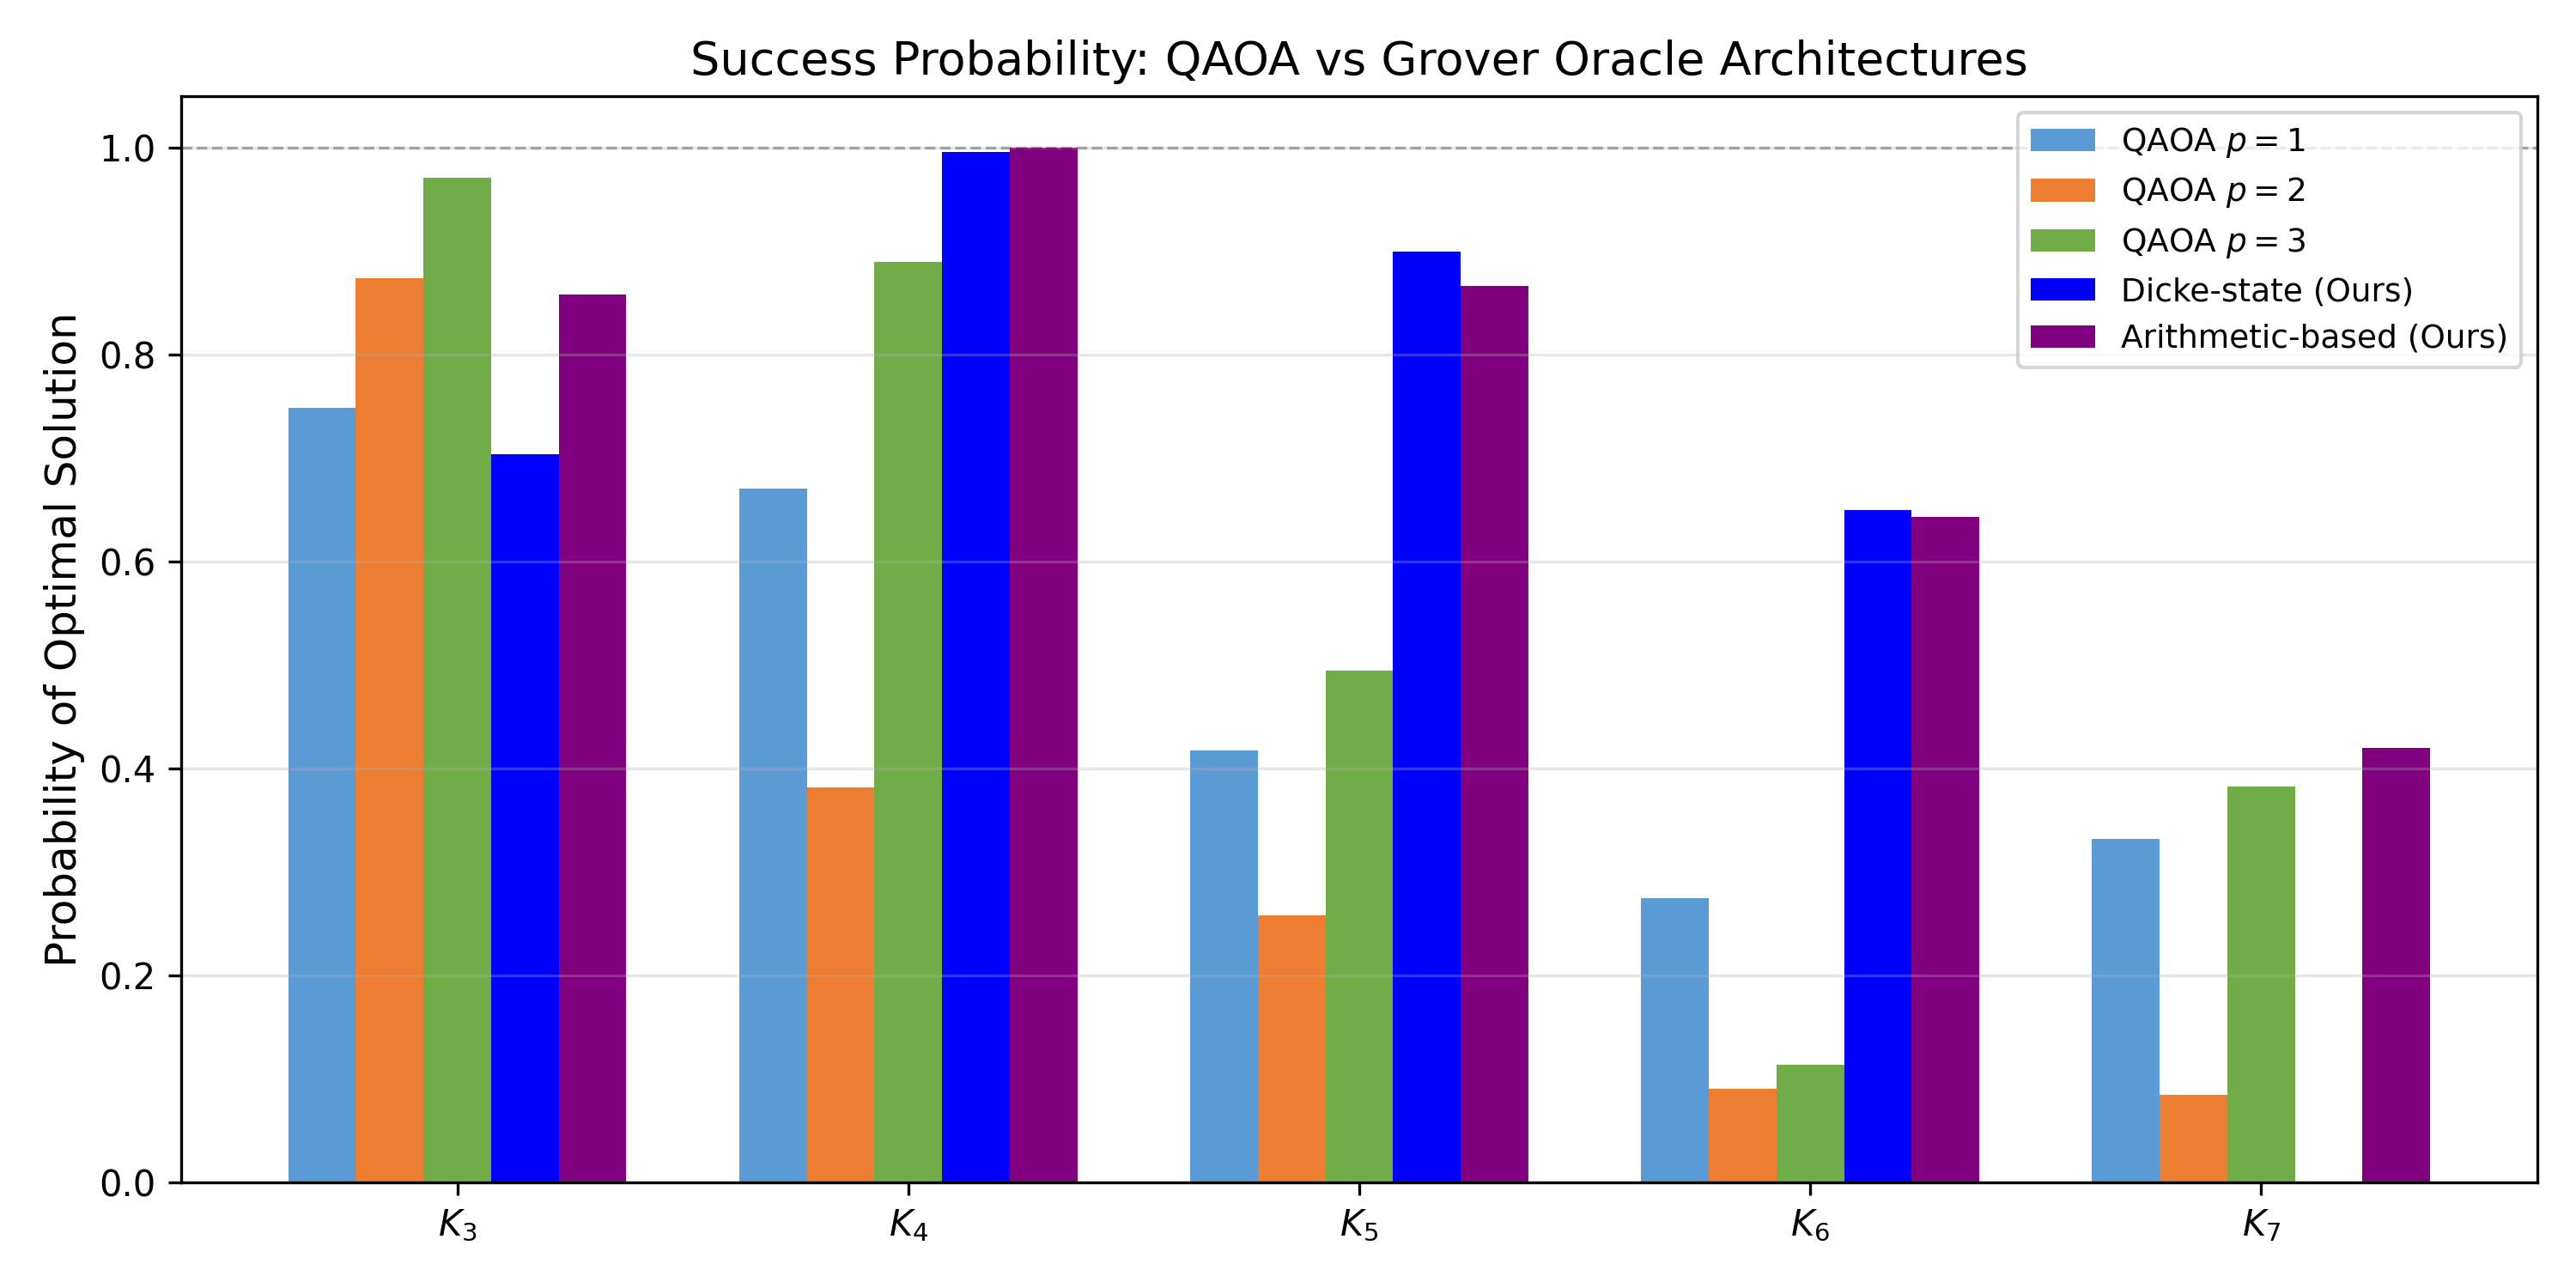
\includegraphics[width=\columnwidth]{figures/fig_success_probability_comparison.png}
\caption{Success probability (probability of measuring
an optimal solution) for QAOA ($p=1,2,3$) versus our
Grover oracle architectures. Grover concentrates
amplitude on the optimal manifold, whereas QAOA's
soft-penalty QUBO bleeds probability mass into
suboptimal high-weight configurations. Note that QAOA
$p=3$ outperforms Grover on $K_3$ due to the simple
energy landscape of the 3-vertex instance; Grover
architectures dominate for $n \geq 4$. Dicke-state
simulation for $K_7$ was not performed due to memory
constraints (30 qubits).}
\label{fig:qaoa_success}
\end{figure}

\begin{figure}[t!]
\centering
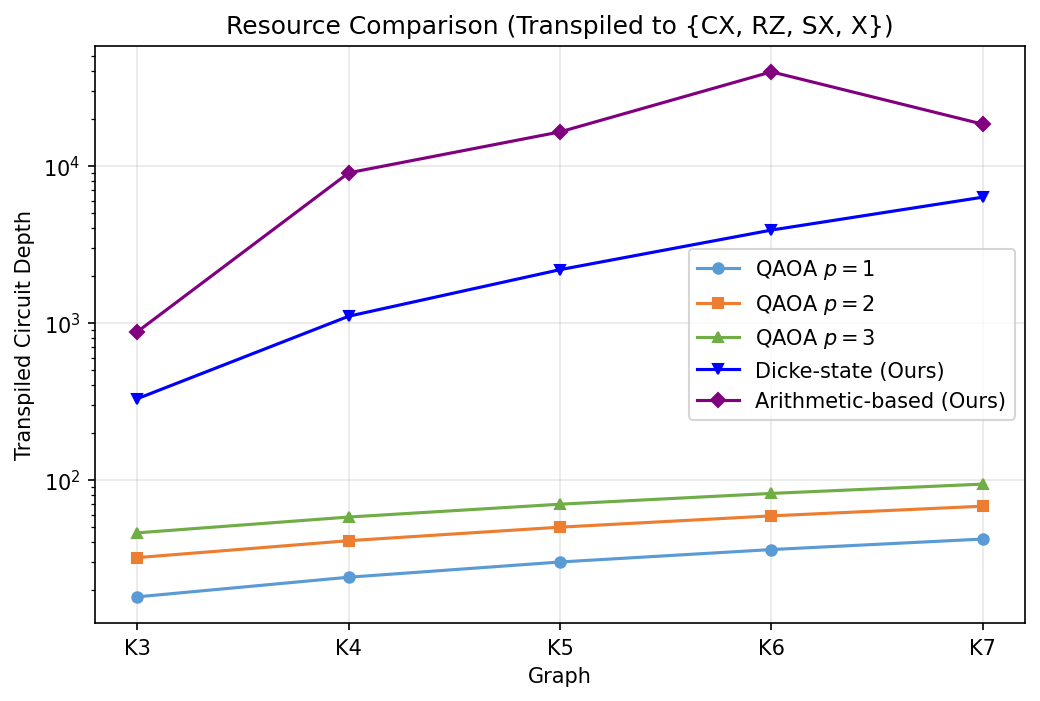
\includegraphics[width=\columnwidth]{figures/fig_depth_comparison.png}
\caption{Transpiled circuit depth comparison (basis:
$\{CX, RZ, SX, X\}$). QAOA achieves the shallowest
circuits at $p=1$ but must increase $p$ for improved
success probability. Our Grover architectures incur
substantially higher transpiled depth due to
multi-controlled gate decomposition, with
Arithmetic-based (Ours) trading depth for logarithmic
ancilla scaling. Note the logarithmic scale on the
vertical axis.}
\label{fig:qaoa_depth}
\end{figure}

\begin{figure}[t!]
\centering
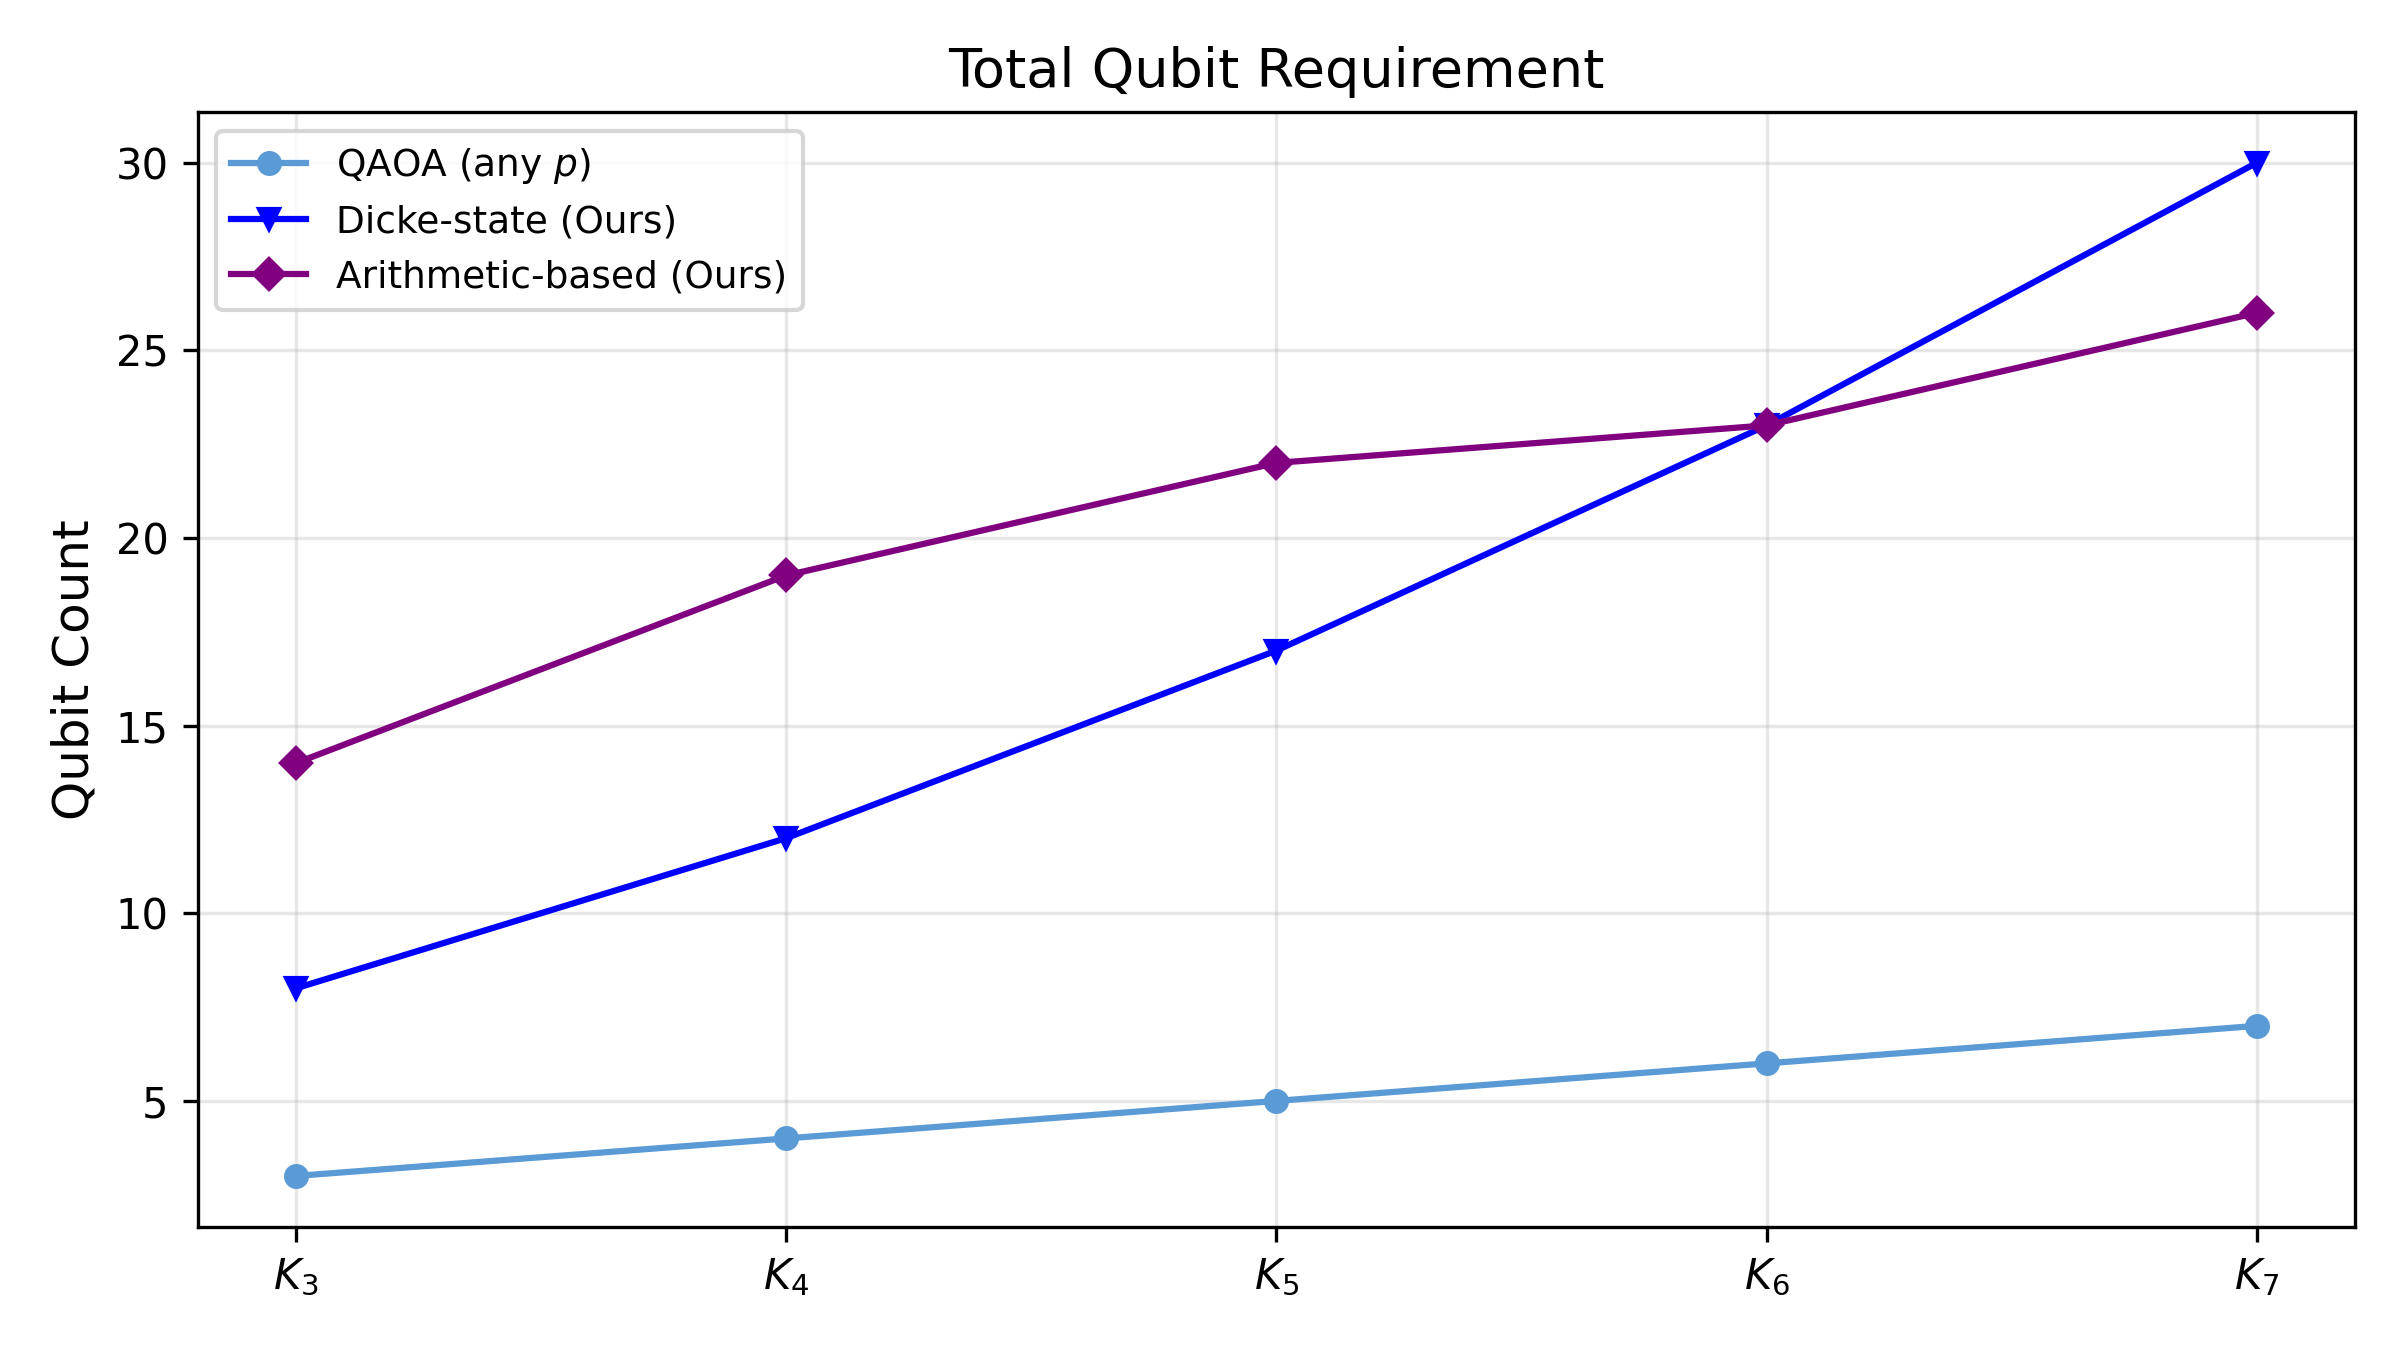
\includegraphics[width=\columnwidth]{figures/fig_qubit_comparison.png}
\caption{Total qubit requirement comparison. QAOA uses
only $n$ qubits regardless of $p$, while
Arithmetic-based (Ours) compresses ancillas to
$O(\log m)$ and Dicke-state (Ours) requires $O(m)$
ancillas for edge checking. Comparison is made under
a resource-unconstrained setting; see
Section~\ref{sec:qaoa_comparison}.}
\label{fig:qaoa_qubits}
\end{figure}

\section{Discussion}
\label{sec:discussion}
The three architectures presented in this work represent distinct design philosophies in the pursuit of qubit-efficient quantum solutions for the Minimum Vertex Cover problem. Each approach offers unique advantages and suffers from specific limitations that must be carefully considered when selecting an appropriate solver for a given application context.

\subsection{Arithmetic vs. Dicke-State Architectures}
The primary trade-off discovered in this research is between qubit count and circuit depth. The Dicke-state approach provides a geometric filter that reduces the search space size, leading to fewer Grover iterations. However, it requires $O(m)$ ancillas for edge checking. The arithmetic approach (including the weighted variant) uses a logarithmic number of qubits for edges but increases circuit depth due to carry propagation in quantum adders.

For sparse graphs where $m \ll n^2$, the Dicke-state architecture offers a compelling advantage. The linear ancilla scaling $m$ remains manageable, while the geometric filtering provides exponential reduction in the effective search space. This makes the Dicke-state approach particularly suitable for applications involving road networks, social networks, or other real-world graphs with low edge density. The reduction from $2^n$ to $\sum_{i=0}^{k}\binom{n}{i}$ states means that for a graph with $n=50$ vertices and seeking a cover of size $k=5$, the search space shrinks from approximately $1.13 \times 10^{15}$ to just $2,369,936$ states—a reduction of over eight orders of magnitude.

Conversely, for dense graphs where $m \approx n^2/2$, the arithmetic architectures become indispensable. The logarithmic edge scaling $O(\log m)$ means that a complete graph with 50 vertices requires only 32 ancilla qubits for edge counting in the arithmetic approach, compared to 1,225 ancilla qubits in the Dicke-state approach. This dramatic reduction in qubit requirements can mean the difference between an implementable circuit and one that exceeds the capabilities of current quantum hardware. Our simulations successfully scaled to $K_7$ using 26 qubits, representing the upper bound of classical simulation for the high-depth arithmetic circuits on standard high-performance backends.

The circuit depth implications are equally significant. The Dicke-state oracle requires a single multi-controlled gate to validate all edges simultaneously, resulting in $O(m)$ gate depth but with a simple structure amenable to optimization. The arithmetic oracle, by contrast, requires sequential penalty additions for each uncovered edge, followed by carry propagation through the comparator circuit. This results in $O(m \cdot \log n)$ gate operations per oracle call. For NISQ devices with limited coherence times, this trade-off between qubit count and circuit depth must be carefully evaluated. Fig. \ref{fig:depth_scaling} and Table \ref{tab:depth_scaling} provide a quantitative comparison of circuit depth scaling across all architectures. Notably, Cherif et al.'s combinatorial penalty term $\binom{n}{k+1}$ grows exponentially with $k$, resulting in severe depth blowup for large graphs. Wang \cite{wang_quantum_2023} and Jiang \& Yan achieve polynomial depth at $O(n^2)$ and $O(n \log n + m)$ respectively. Our Dicke-state architecture achieves $O(nk^2 + m)$; however, when $k \approx \sqrt{n}$, this depth can exceed that of Wang et al.'s $O(n^2)$ approach. The $k^2$ factor is mitigated when $k \ll n$, making the Dicke-state architecture advantageous in the sparse regime where the optimal cover size is small relative to $n$. Furthermore, the arithmetic circuit depth can vary non-monotonically with $n$: in our benchmarks, $K_7$ exhibited lower depth than $K_6$ because the penalty $P = n+1 = 8$ is a power of two, requiring fewer binary decomposed controlled-increments per uncovered edge despite the larger edge count.

\subsection{Limitations of Dicke-State Preparation}
Our analysis reveals a fundamental limitation of GDSP in the context of Weighted MVC. Since $|D_{\le k}^n\rangle$ treats all vertices as having equal weight, it cannot bias the search space towards lower-cost configurations in the weighted case. Therefore, arithmetic weight-summing remains the only viable path for generalized cost functions.

Furthermore, the Dicke-state architecture requires a priori knowledge of an upper bound $k$ on the minimum vertex cover size. If $k$ is set too low, the algorithm will fail to find any valid solution. If $k$ is set too high, the benefits of search space reduction are diminished. In practice, estimating $k$ may require classical pre-processing or domain knowledge about the specific graph structure.

Another limitation concerns the precision of Dicke state preparation. The algorithm by Narisada et al. requires computing precise rotation angles from binomial distribution coefficients. For large $n$, numerical precision in classical pre-computation becomes critical, and any errors can propagate to incorrect state preparation, reducing the probability of measuring valid solutions.

\subsection{Generality vs. Overhead in Weighted Instances}

The Weighted Arithmetic architecture represents the most generalized solution, bridging the gap between theoretical quantum algorithms and practical operations research, where vertices invariably carry heterogeneous costs (e.g., financial costs in resource allocation, or server capacities in network routing). 

However, this generality introduces specific overheads. Unlike the unweighted arithmetic solver, the counter register size must scale to accommodate the sum of all arbitrary weights $\lceil\log_2(\sum w_i + (\sum w_i + 1)m + 1)\rceil$. While this scaling remains logarithmic with respect to the total weight, the gate synthesis for adding arbitrary binary values requires more complex multi-controlled configurations than simple unitary increments. Therefore, for unweighted instances, utilizing the standard arithmetic architecture is strictly preferable to avoid unnecessary gate depth overhead.

\subsection{NISQ-Era Considerations and Hybrid Optimization}
The practical implementation of these architectures on current quantum hardware introduces additional considerations beyond theoretical qubit and gate scaling. Noise in NISQ devices manifests as decoherence, gate errors, and measurement errors, each of which affects the three architectures differently.

The Dicke-state architecture, while qubit-efficient for sparse graphs, requires high-depth circuits for state preparation. The multi-stage process of input superposition and Dicke expansion involves numerous two-qubit gates, making it susceptible to accumulated gate errors. Furthermore, the final multi-controlled-X gate for edge validation may require significant decomposition depth when transpiled for hardware with limited connectivity.

The arithmetic architectures face similar challenges from the quantum adder circuits. Carry propagation in the comparator introduces correlated errors across multiple qubits, and the sequential nature of penalty addition means that errors can accumulate throughout the oracle execution. However, the reduced qubit count may allow for implementation on smaller, higher-quality quantum processors where error rates are typically lower.

To mitigate these NISQ limitations, the \textbf{Skip-K optimization} proves to be an essential classical-quantum hybrid mechanism. By leveraging early measurement results to aggressively lower the pivot threshold, Skip-K drastically reduces the total number of Grover iterations required. Interestingly, in a noisy environment, device noise may occasionally induce a state collapse to a valid, low-weight cover even when testing at a high pivot value. The Skip-K algorithm can capitalize on these serendipitous discoveries to skip large segments of the search space, effectively turning a NISQ hardware flaw into a heuristic advantage.

\subsection{Grover vs. QAOA: Deterministic Oracles vs. Variational Heuristics}
The QAOA baseline comparison in Section \ref{sec:qaoa_comparison} reveals that \emph{success probability}---the probability of actually measuring an optimal solution---is the decisive metric for constrained combinatorial optimization. QAOA's soft QUBO penalty term competes with the objective term, causing the mixer Hamiltonian to disproportionately populate high-Hamming-weight states such as the all-1's configuration. Even when the best observed cost equals the true minimum, the majority of measurement shots may be wasted on suboptimal covers. Furthermore, QAOA requires a classical optimization loop (in our benchmarks, $80 \times 4096 \times 5 \approx 1.6 \times 10^6$ shots just for parameter training) whose cost landscape is non-convex and highly sensitive to initial guesses.

By contrast, Grover's deterministic oracle eliminates both of these failure modes. No classical optimization is required: the iteration count is analytically determined from the search-space size. More importantly, every state amplified by the oracle is guaranteed to satisfy the hard vertex-cover constraint. On NISQ hardware, where every additional gate increases error probability, the certainty that each measured state is valid provides a significant practical advantage over variational heuristics that must statistically ``discover'' feasibility.

\subsection{Selection Guidelines}

Based on our comprehensive analysis, we establish the following roadmap for selecting the optimal MVC solver architecture:
\begin{itemize}
    \item \textbf{Dicke-State Architecture:} Optimal for \textit{unweighted, sparse graphs} where a reasonable upper bound $k$ is known. It provides the shallowest effective search depth.
    \item \textbf{Arithmetic-Based Architecture:} Optimal for \textit{unweighted, dense graphs}. It provides the best qubit scalability ($O(\log m)$) to overcome severe hardware size limitations.
    \item \textbf{Weighted Arithmetic Architecture:} The mandatory selection for \textit{weighted instances} (WMVC) with heterogeneous costs, highly dependent on the Skip-K framework to manage its large solution space.
\end{itemize}
Future work should explore hardware-specific transpilation and error mitigation techniques tailored to the unique circuit structures of each proposed architecture.


\section{Conclusion}
\label{sec:conclusion}

This paper presented and evaluated three qubit-efficient quantum circuit architectures for solving the Minimum Vertex Cover (MVC) problem and its weighted variant (WMVC) using Grover's search algorithm. We traced an architectural progression from search space filtering via Generalized Dicke State Preparation to highly scalable arithmetic-based edge validation. 

Our analysis reveals that while the Dicke-state architecture offers rapid convergence for sparse graphs, its $O(m)$ ancilla requirement fundamentally limits its scalability on dense networks. In contrast, the arithmetic architectures overcome this bottleneck by employing binary counters and the Cuccaro comparator, drastically reducing the edge validation overhead to $O(\log m)$ qubits. Furthermore, the weighted arithmetic architecture extends this framework to natively handle heterogeneous vertex costs, bridging the gap between theoretical quantum search and practical operations research. 

A critical contribution of this work is the integration of the \textbf{Skip-K optimization}---a classical-quantum hybrid measurement feedback mechanism that dynamically skips redundant pivot values, thereby significantly accelerating the search process across all three architectures. 

By systematically delineating the critical trade-offs between spatial qubit scaling and temporal circuit depth, this study provides a concrete roadmap for deploying quantum combinatorial optimization on near-term hardware. Future work will investigate the application of mid-circuit measurement and dynamic qubit reuse to further compress the spatial requirements of these solvers, alongside hardware-aware transpilation and error mitigation techniques to maximize their performance on noisy quantum processors.

\appendices
\section{Simulation Results}
The following figures provide the complete state-vector simulation results and probability distributions for the evaluated benchmark graphs across different architectures.

\begin{figure*}[!bph]
\centering
\begin{minipage}{\textwidth}
    \centering
    \subfloat[Dicke-state ($K_3$, pivot=3)]%
        {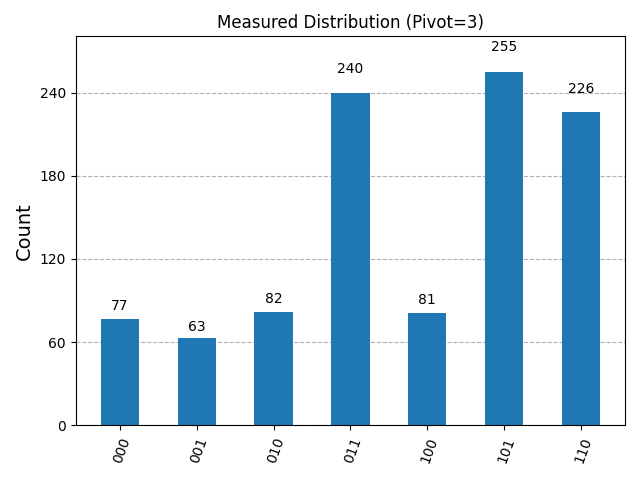
\includegraphics[width=0.48\textwidth]{figures/distribution_K3_pivot3_dicke_01.png}\label{fig:k3_dicke}}
    \hfill
    \subfloat[Arithmetic ($K_3$, pivot=3)]%
        {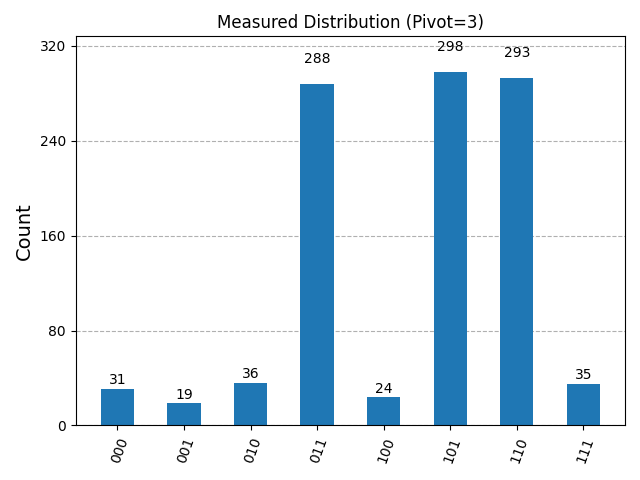
\includegraphics[width=0.48\textwidth]{figures/distribution_K3_pivot3_arith_01.png}\label{fig:k3_arith}}
\end{minipage}
\caption{Comparison of solution distributions for $K_3$ (MVC=2) using Dicke-state and arithmetic architectures.\label{fig:k3_comparison}}
\end{figure*}

\begin{figure*}[!bph]
\centering
\begin{minipage}{\textwidth}
    \centering
    \subfloat[Dicke-state ($K_4$, pivot=4)]%
        {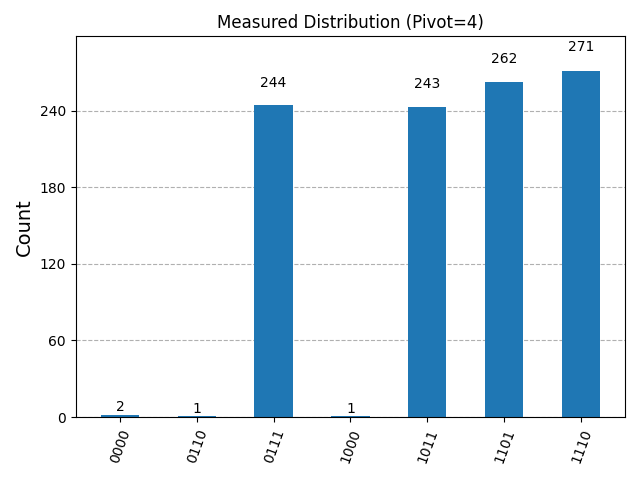
\includegraphics[width=0.48\textwidth]{figures/distribution_K4_pivot4_dicke_01.png}\label{fig:k4_dicke}}
    \hfill
    \subfloat[Arithmetic ($K_4$, pivot=4)]%
        {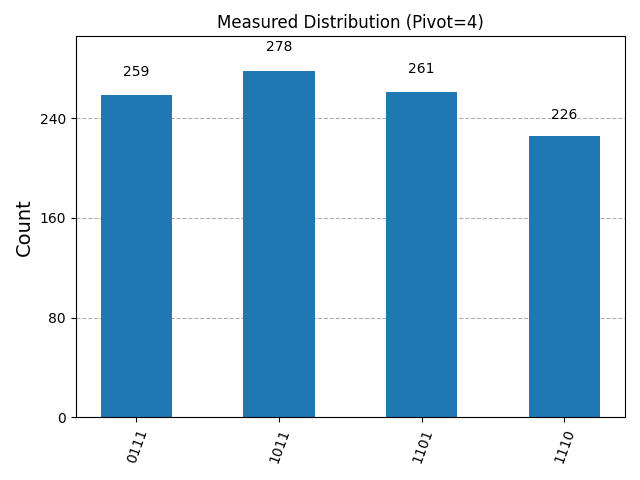
\includegraphics[width=0.48\textwidth]{figures/distribution_K4_pivot4_arith_01.png}\label{fig:k4_arith}}
\end{minipage}
\caption{Comparison of solution distributions for $K_4$ (MVC=3) using Dicke-state and arithmetic architectures.\label{fig:k4_comparison}}
\end{figure*}

\begin{figure*}[!bph]
\centering
\begin{minipage}{\textwidth}
    \centering
    \subfloat[Dicke-state ($K_5$, pivot=5)]%
        {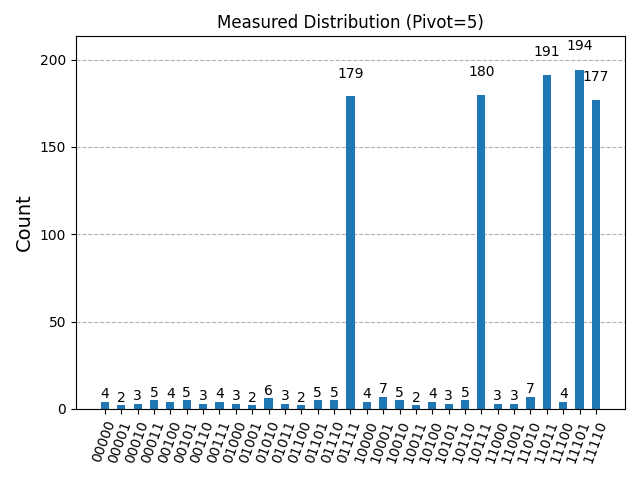
\includegraphics[width=0.48\textwidth]{figures/distribution_K5_pivot5_dicke_01.png}\label{fig:k5_dicke}}
    \hfill
    \subfloat[Arithmetic ($K_5$, pivot=5)]%
        {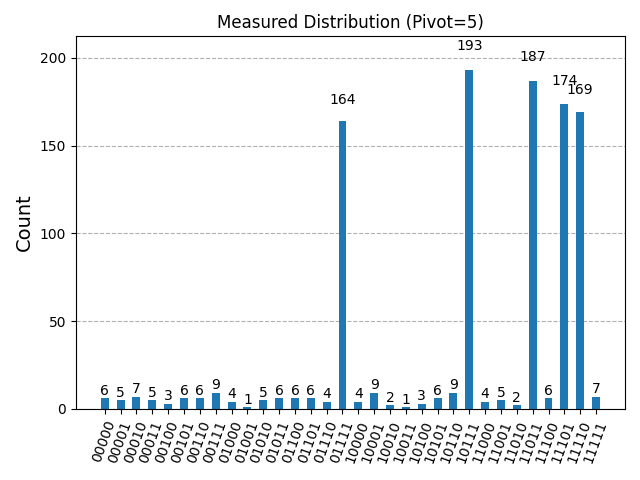
\includegraphics[width=0.48\textwidth]{figures/distribution_K5_pivot5_arith_01.png}\label{fig:k5_arith}}
\end{minipage}
\caption{Comparison of solution distributions for $K_5$ (MVC=4) using Dicke-state and arithmetic architectures.\label{fig:k5_comparison}}
\end{figure*}

\begin{figure*}[!bph]
\centering
\begin{minipage}{\textwidth}
    \centering
    \subfloat[Dicke-state ($K_6$, pivot=6)]%
        {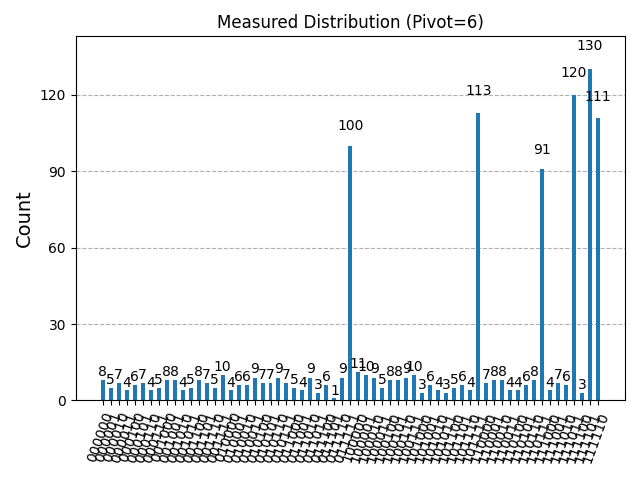
\includegraphics[width=0.48\textwidth]{figures/distribution_K6_pivot6_dicke_01.png}\label{fig:k6_dicke}}
    \hfill
    \subfloat[Arithmetic ($K_6$, pivot=6)]%
        {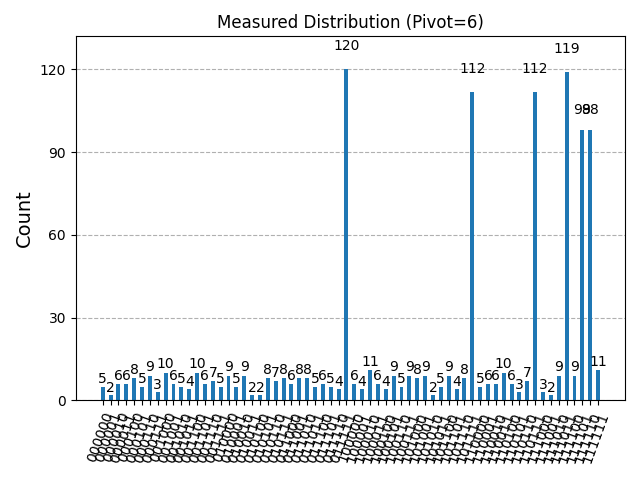
\includegraphics[width=0.48\textwidth]{figures/distribution_K6_pivot6_arith_01.png}\label{fig:k6_arith}}
\end{minipage}
\caption{Comparison of solution distributions for $K_6$ (MVC=5) using Dicke-state and arithmetic architectures.\label{fig:k6_comparison}}
\end{figure*}

\begin{figure*}[!bph]
\centering
\begin{minipage}{\textwidth}
    \centering
    \subfloat[Dicke-state ($C_4$, pivot=3)]%
        {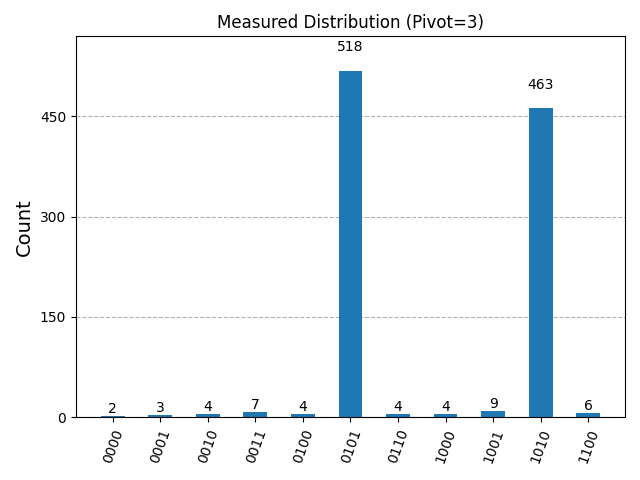
\includegraphics[width=0.48\textwidth]{figures/distribution_cycle_C4_dicke_01.png}\label{fig:c4_dicke}}
    \hfill
    \subfloat[Arithmetic ($C_4$, pivot=3)]%
        {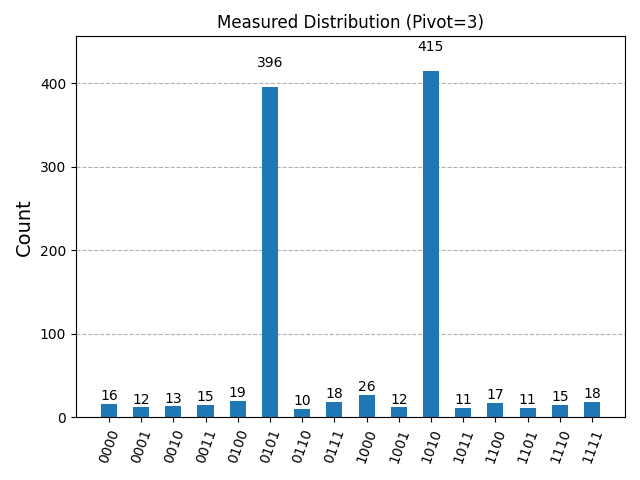
\includegraphics[width=0.48\textwidth]{figures/distribution_cycle_C4_arith_01.png}\label{fig:c4_arith}}
\end{minipage}
\caption{Comparison of solution distributions for $C_4$ (MVC=2) using Dicke-state and arithmetic architectures.\label{fig:c4_comparison}}
\end{figure*}

\begin{figure*}[!bph]
\centering
\begin{minipage}{\textwidth}
    \centering
    \subfloat[Dicke-state ($C_5$, pivot=4)]%
        {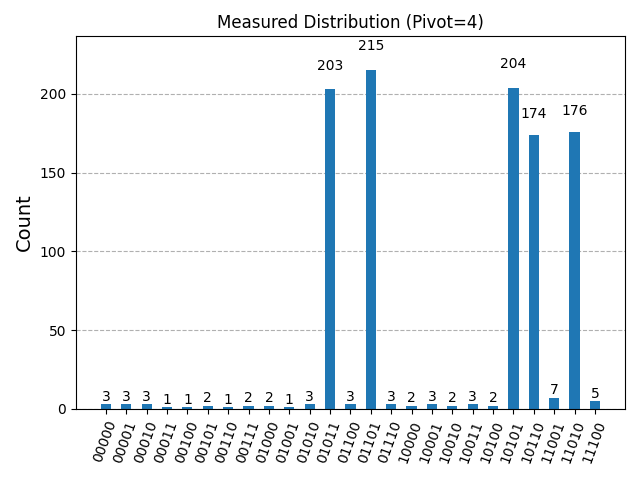
\includegraphics[width=0.48\textwidth]{figures/distribution_cycle_C5_dicke_01.png}\label{fig:c5_dicke}}
    \hfill
    \subfloat[Arithmetic ($C_5$, pivot=4)]%
        {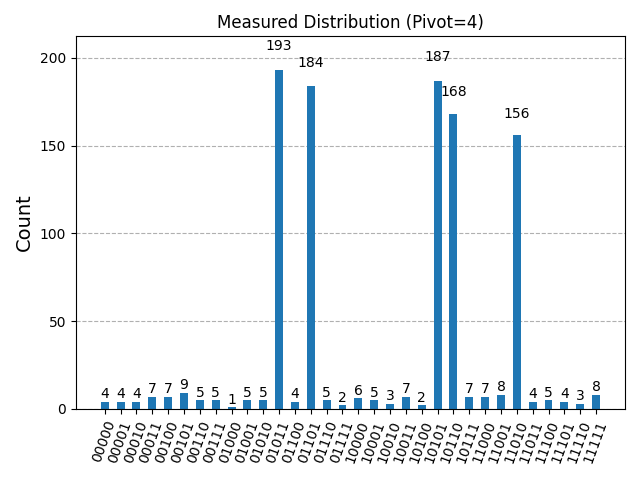
\includegraphics[width=0.48\textwidth]{figures/distribution_cycle_C5_arith_01.png}\label{fig:c5_arith}}
\end{minipage}
\caption{Comparison of solution distributions for $C_5$ (MVC=3) using Dicke-state and arithmetic architectures.\label{fig:c5_comparison}}
\end{figure*}

\begin{figure*}[!bph]
\centering
\begin{minipage}{\textwidth}
    \centering
    \subfloat[Dicke-state ($C_6$, pivot=4)]%
        {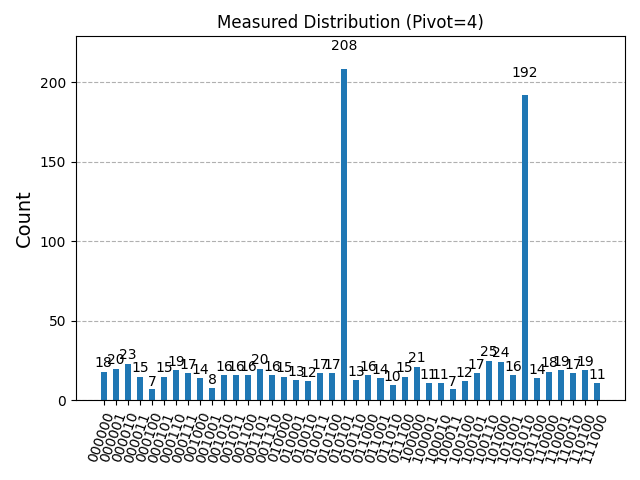
\includegraphics[width=0.48\textwidth]{figures/distribution_cycle_C6_dicke_01.png}\label{fig:c6_dicke}}
    \hfill
    \subfloat[Arithmetic ($C_6$, pivot=4)]%
        {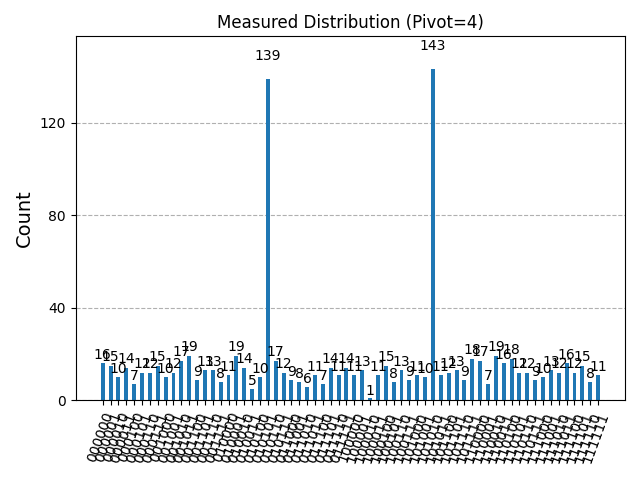
\includegraphics[width=0.48\textwidth]{figures/distribution_cycle_C6_arith_01.png}\label{fig:c6_arith}}
\end{minipage}
\caption{Comparison of solution distributions for $C_6$ (MVC=3) using Dicke-state and arithmetic architectures.\label{fig:c6_comparison}}
\end{figure*}

\begin{figure}[htbp]
\centering
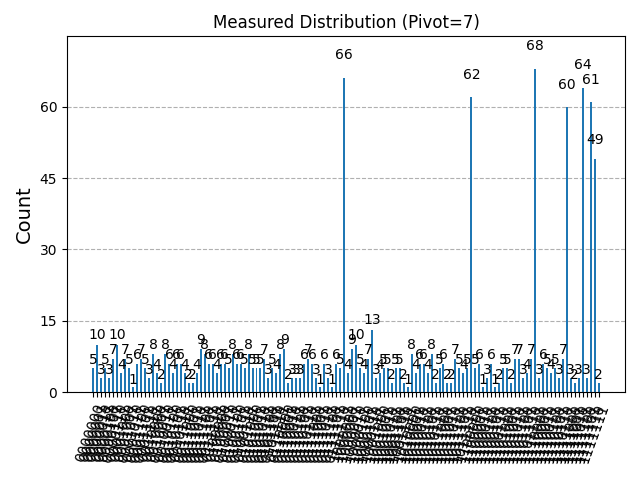
\includegraphics[width=0.45\textwidth]{figures/distribution_K7_pivot7_arith_01.png}
\caption{Solution distribution for $K_7$ (MVC=6, pivot=7) using the arithmetic architecture. Dicke-state simulation was not possible due to qubit requirements exceeding classical simulation capacity.\label{fig:k7_comparison}}
\end{figure}

\begin{figure}[htbp]
\centering
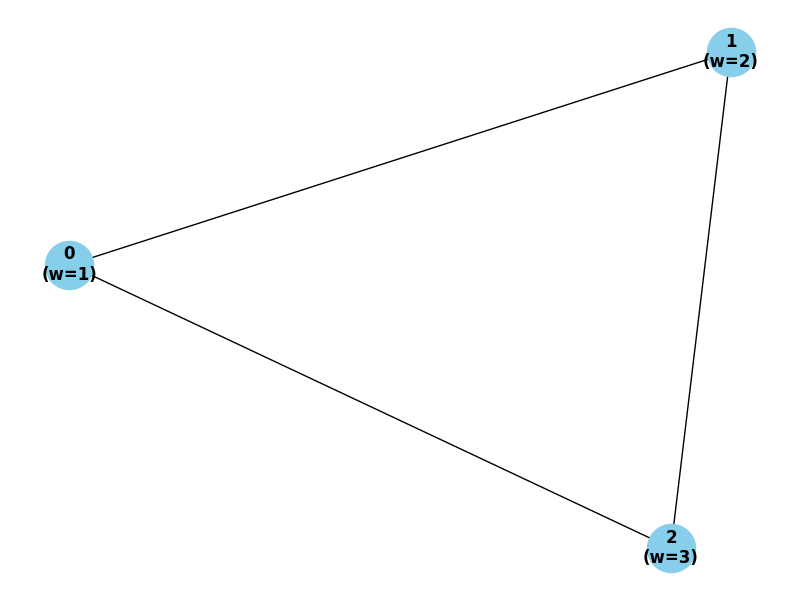
\includegraphics[width=0.3\textwidth]{figures/graph_weighted_K3_123_01.png}
\caption{Weighted $K_3$ problem instance with vertex weights $w_0=1, w_1=2, w_2=3$.\label{fig:weighted_graph}}
\end{figure}

\begin{figure}[htbp]
\subfloat[$K_3$ weights (1,2,3), MVC=3, pivot=4]{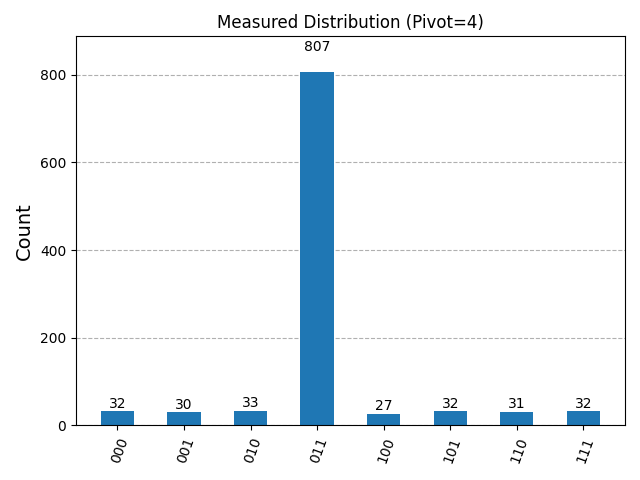
\includegraphics[width=0.32\textwidth]{figures/distribution_weighted_K3_123_01.png}\label{fig:dist_weighted_k3}}
\hfill
\subfloat[$P_4$ weights (1,2,3,4), MVC=5, pivot=6\label{fig:dist_weighted_p4}]{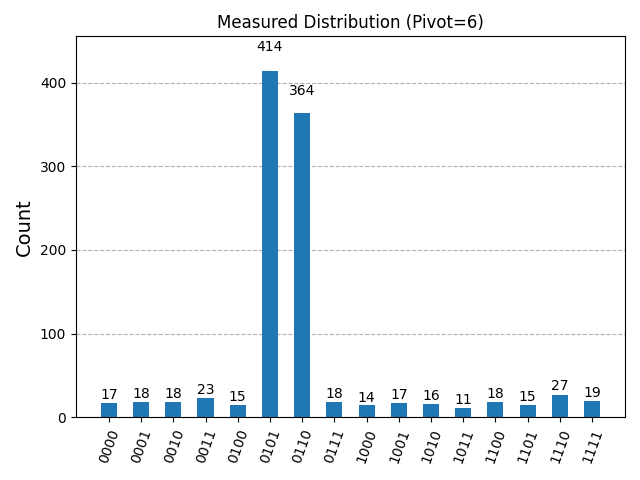
\includegraphics[width=0.32\textwidth]{figures/distribution_weighted_P4_1234_01.png}}
\hfill
\subfloat[$S_4$ weights (1,1,10,10), MVC=1, pivot=2\label{fig:dist_weighted_s4}]{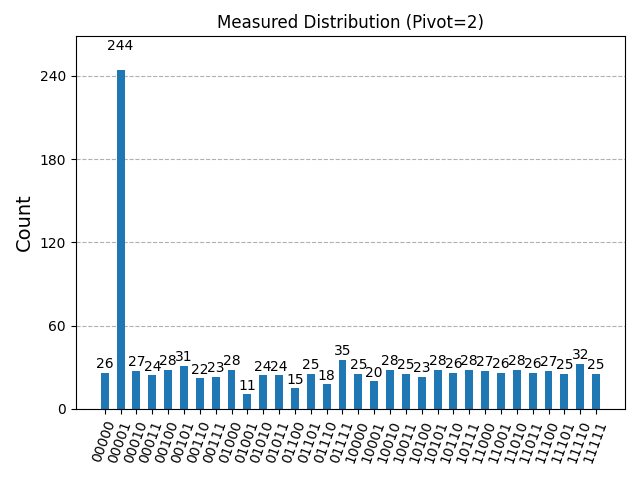
\includegraphics[width=0.32\textwidth]{figures/distribution_weighted_S4_111010_01.png}}
\caption{Weighted vertex cover results: problem instances and solution distributions.\label{fig:dist_weighted}}
\end{figure}

\begin{figure}[htbp]
\centering
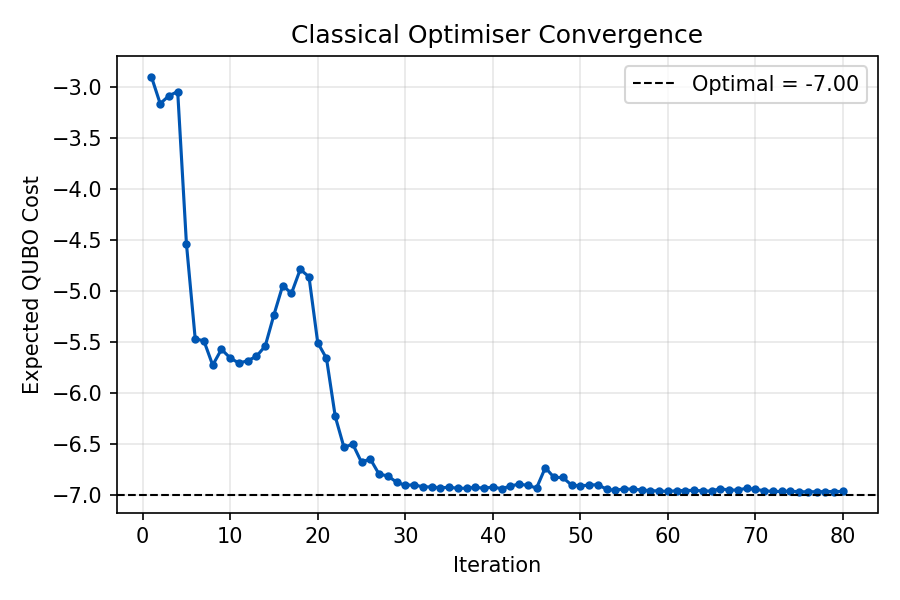
\includegraphics[width=0.75\columnwidth]{figures/qaoa_convergence_K3_p3.png}
\caption{QAOA $p=3$ SPSA convergence trajectory for $K_3$ (MVC=2).\label{fig:qaoa_conv_k3}}
\end{figure}

\begin{figure}[htbp]
\centering
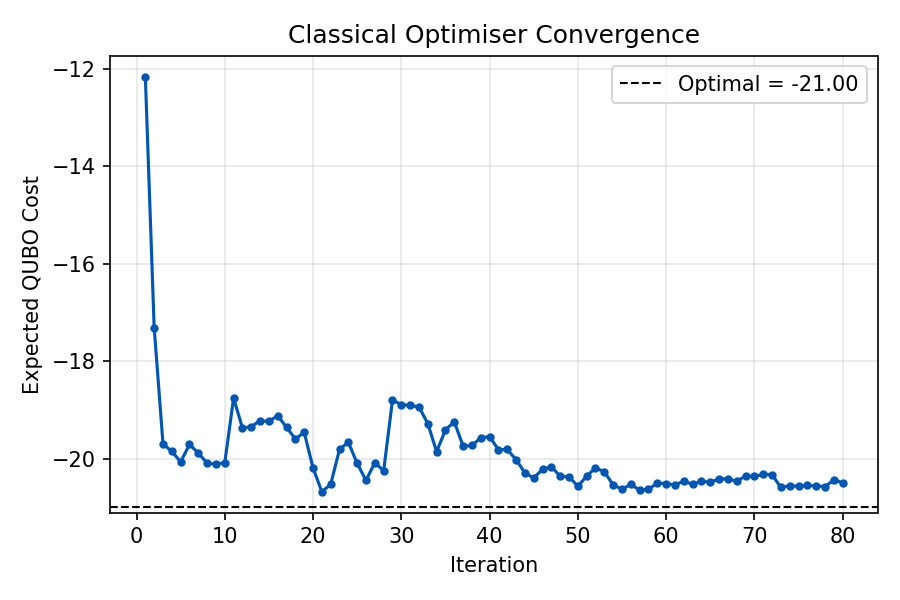
\includegraphics[width=0.75\columnwidth]{figures/qaoa_convergence_K4_p3.png}
\caption{QAOA $p=3$ SPSA convergence trajectory for $K_4$ (MVC=3).\label{fig:qaoa_conv_k4}}
\end{figure}

\begin{figure}[htbp]
\centering
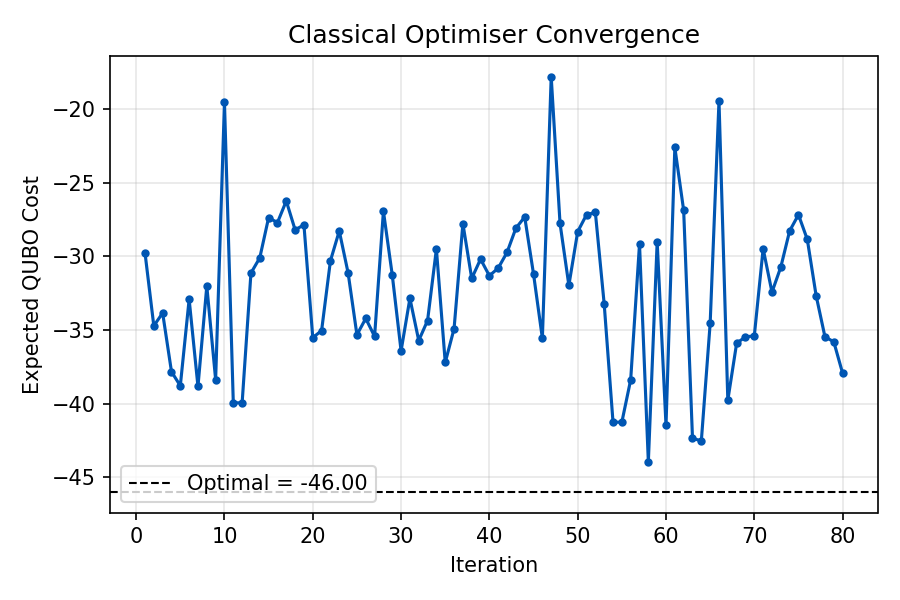
\includegraphics[width=0.75\columnwidth]{figures/qaoa_convergence_K5_p3.png}
\caption{QAOA $p=3$ SPSA convergence trajectory for $K_5$ (MVC=4).\label{fig:qaoa_conv_k5}}
\end{figure}

\begin{figure}[htbp]
\centering
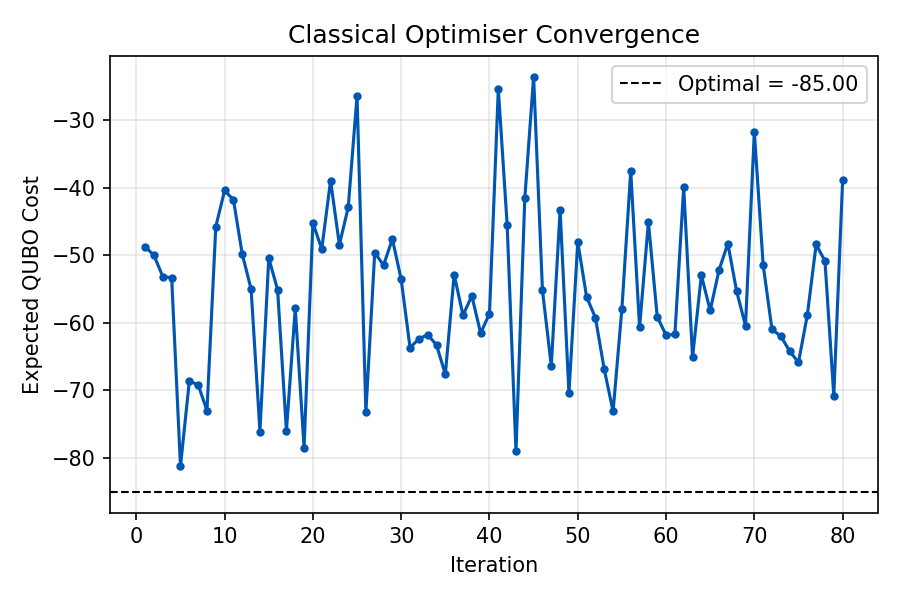
\includegraphics[width=0.75\columnwidth]{figures/qaoa_convergence_K6_p3.png}
\caption{QAOA $p=3$ SPSA convergence trajectory for $K_6$ (MVC=5).\label{fig:qaoa_conv_k6}}
\end{figure}

\begin{figure}[htbp]
\centering
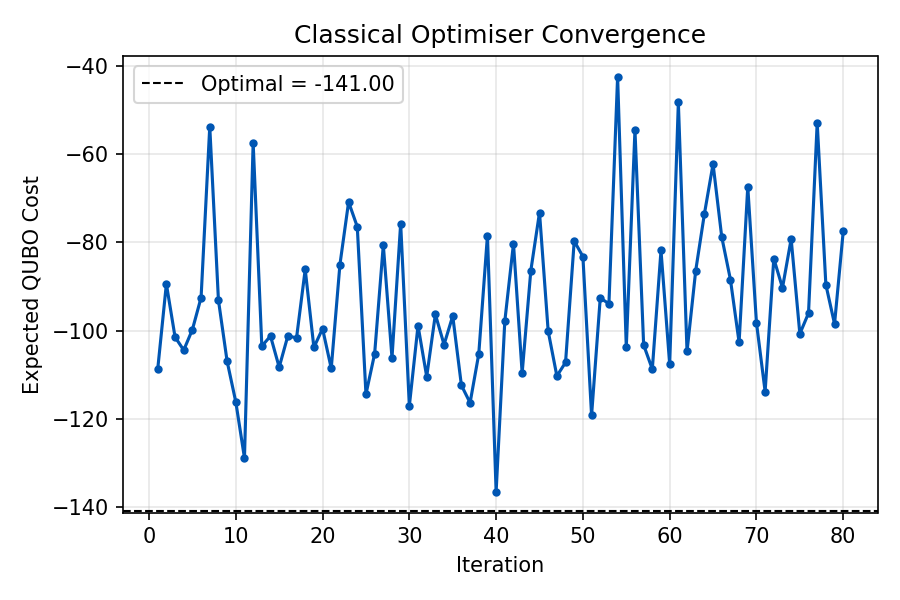
\includegraphics[width=0.75\columnwidth]{figures/qaoa_convergence_K7_p3.png}
\caption{QAOA $p=3$ SPSA convergence trajectory for $K_7$ (MVC=6).\label{fig:qaoa_conv_k7}}
\end{figure}
\clearpage

\section*{Acknowledgment}
The authors thank the Qiskit development team and IBM Quantum for providing access to quantum simulators and hardware.

\bibliographystyle{ieeetr}
\bibliography{exported-items}

\begin{IEEEbiography}[{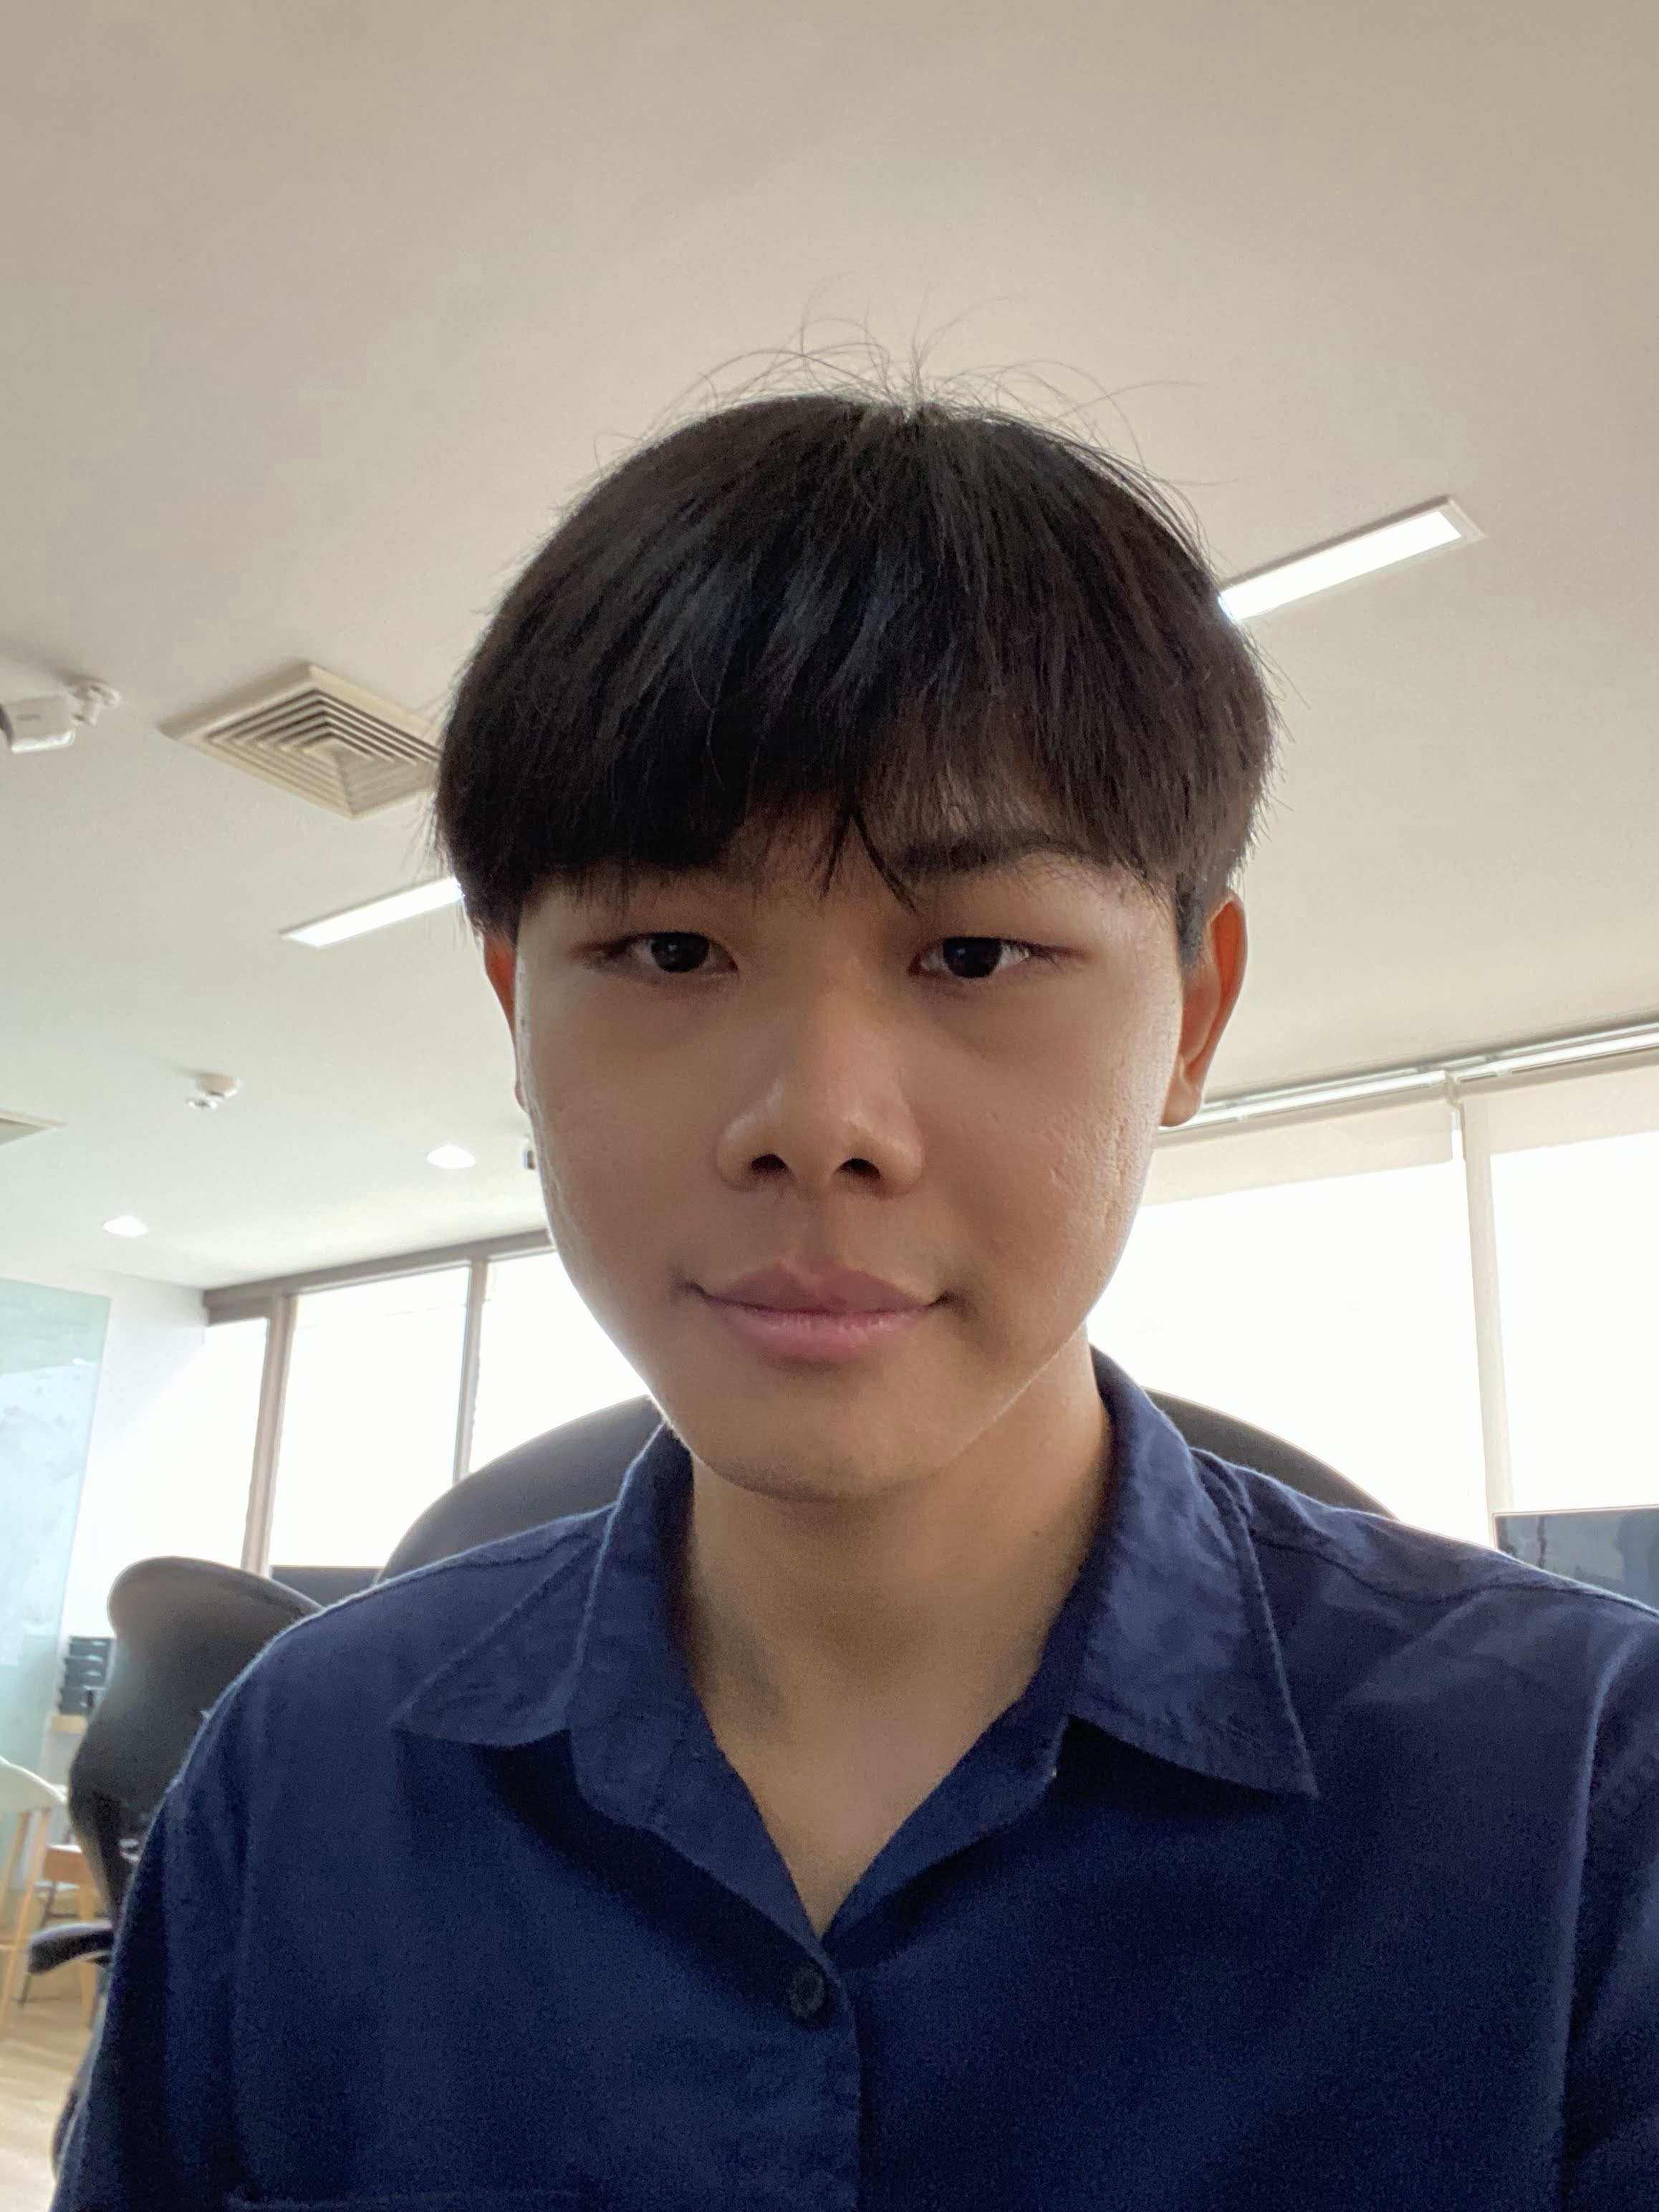
\includegraphics[width=1in,height=1.25in,clip,keepaspectratio]{figures/krissada.jpg}}]{Krissada Sarawit} is a graduate student in the Department of Computer Engineering, Faculty of Engineering, Chulalongkorn University, Thailand. His research focuses on quantum computing algorithms and quantum circuit optimization.
\end{IEEEbiography}

\vspace{-30em}

\begin{IEEEbiography}[{
\includegraphics[width=1in,height=1.25in,clip,keepaspectratio]{figures/kamonluk.jpg}}]{Kamonluk Suksen} received her B.Eng., M.Eng., and Ph.D. degrees in Computer Engineering from Chulalongkorn University in 2013, 2014, and 2022, respectively. After graduation, she worked as a process engineer and software engineer at a company specializing in visual effects and computer graphics for feature films and advertising, where she focused on workflow optimization and the development of internal software tools. She is currently a lecturer in Computer Engineering at Chulalongkorn University. Her research interests are primarily in quantum computing and quantum algorithms for optimization problems, with an emphasis on bridging theory and practical applications.
\end{IEEEbiography}


\EOD

\end{document}
